\documentclass[11pt,a4paper,openany]{book}
\usepackage[utf8]{inputenc}
\usepackage[T1]{fontenc}
\usepackage[spanish,es-tabla]{babel}
\usepackage{lmodern}
\usepackage[top=2.5cm,bottom=2.5cm,left=2.5cm,right=2.5cm,headheight=14pt]{geometry}
\usepackage{microtype}
\usepackage[table,xcdraw]{xcolor}
\definecolor{headerblue}{RGB}{24,43,73}
\definecolor{accentblue}{RGB}{30,80,150}
\definecolor{lightbg}{RGB}{248,249,251}
\definecolor{bordergray}{RGB}{220,224,230}
\definecolor{darktext}{RGB}{33,37,41}
\definecolor{codebg}{RGB}{245,247,250}
\definecolor{commentgreen}{RGB}{40,140,70}
\definecolor{keywordpurple}{RGB}{120,40,140}
\usepackage{amsmath,amssymb,amsthm}
\usepackage{graphicx}
\graphicspath{{assets/originales/}{../public/assets/}{./}}
\usepackage{hyperref}
\hypersetup{colorlinks=true,linkcolor=accentblue,citecolor=accentblue,urlcolor=accentblue,pdftitle={LogiLearn -- Informe Tecnico},pdfauthor={UNPRG MATG1001},bookmarksnumbered=true,breaklinks=true}
\usepackage{booktabs,tabularx,array,longtable,enumitem,caption,float}
\usepackage{fancyhdr}
\pagestyle{fancy}
\fancyhf{}
\renewcommand{\headrulewidth}{0.4pt}
\fancyhead[LE,RO]{\small\textsc{LogiLearn -- Informe T\'ecnico}}
\fancyhead[RE,LO]{\small\leftmark}
\fancyfoot[C]{\small\thepage}
\fancypagestyle{plain}{\fancyhf{}\fancyfoot[C]{\small\thepage}\renewcommand{\headrulewidth}{0pt}}
\usepackage{titlesec}
\titleformat{\chapter}[display]{\Huge\bfseries\color{headerblue}}{\chaptername\ \thechapter}{12pt}{\Huge}
\titleformat{\section}{\Large\bfseries\color{headerblue}}{}{0pt}{}
\titleformat{\subsection}{\large\bfseries\color{accentblue}}{}{0pt}{}
\usepackage{listings}
\lstdefinelanguage{TypeScript}{keywords={const,let,function,return,import,export,for,if,else,new,interface,type,extends,switch,case,break,continue,while,try,catch,throw},keywordstyle=\color{keywordpurple}\bfseries,comment=[l]{//},commentstyle=\color{commentgreen}\itshape,sensitive=true}
\lstset{basicstyle=\ttfamily\footnotesize\color{darktext},breaklines=true,frame=single,rulecolor=\color{bordergray},backgroundcolor=\color{codebg},numbers=left,numberstyle=\tiny\color{gray},showstringspaces=false,tabsize=2,extendedchars=true,literate={á}{{\'a}}1 {é}{{\'e}}1 {í}{{\'i}}1 {ó}{{\'o}}1 {ú}{{\'u}}1 {ñ}{{\~n}}1}
\begin{document}
\frontmatter
\begin{titlepage}
\centering
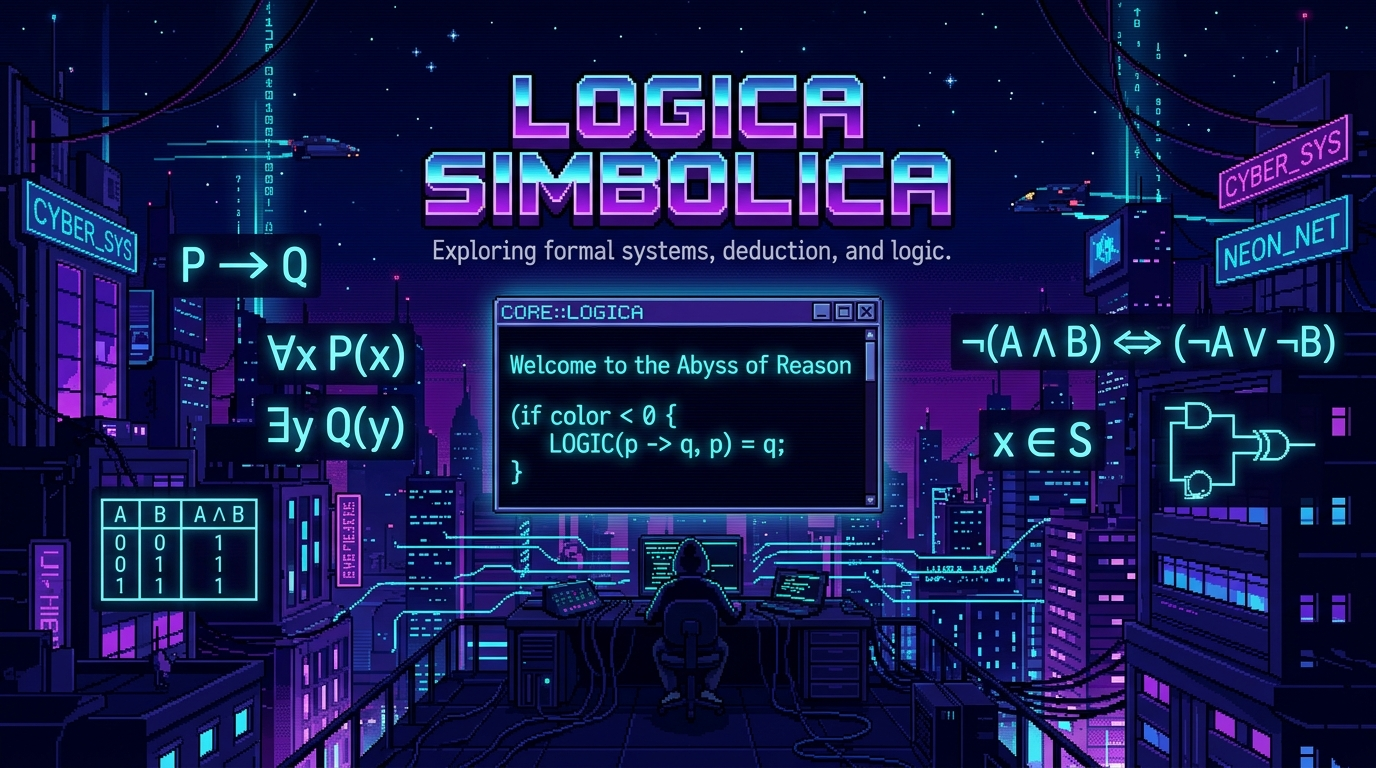
\includegraphics[width=0.55\textwidth]{public_banner.jpg}\par
\vspace{0.6cm}
{\Large Universidad Nacional Pedro Ruiz Gallo\par}
{\large Facultad de Ingenier\'ia Civil, de Sistemas y de Arquitectura\par}
{\large Escuela Profesional de Ingenier\'ia de Sistemas\par}
\vspace{0.9cm}
{\Huge \bfseries\color{headerblue} LogiLearn\par}
{\LARGE L\'ogica Simb\'olica Global\par}
\vspace{0.3cm}
{\large \textbf{Informe T\'ecnico y Documentaci\'on de Sprints}\par}
{\large Arquitectura, motores l\'ogicos y evoluci\'on en 4 semanas $\cdot$ 4 equipos\par}
\vspace{0.8cm}
\begin{center}
\begin{tabular}{ll}
\toprule
\textbf{Curso:} & MATG1001 --- 2026 I, II Ciclo (3 cr\'editos) \\
\textbf{Docente:} & Dr. Mardo Victor Gonzales Herrera \\
\textbf{L\'ider:} & Enrique D\'iaz Cayaca \\
\textbf{Equipos:} & Sinergia $\cdot$ Hijos de Linus $\cdot$ Modus Innova $\cdot$ Linus \\
\textbf{Stack:} & Vue 3 + Vite 6 + TypeScript + Tailwind v4 + Vitest (189 pruebas) \\
\textbf{Repositorio:} & \url{https://github.com/EnriDiazCayaca/logica_simbolica_global} \\
\bottomrule
\end{tabular}
\end{center}
\vspace{0.8cm}
{\small Lambayeque, Per\'u --- Septiembre 2026\par}
\end{titlepage}
\tableofcontents
\listoffigures
\listoftables
\mainmatter

\chapter{Resumen y alcance}
\label{ch:resumen}
LogiLearn implementa el cien por ciento del s\'ilabo MATG1001 con motores reales: tablas de verdad con clasificaci\'on, inferencias con trazabilidad y contraejemplo de $2^{N}$ combinaciones, cuantificadores $\forall$ y $\exists$ sobre dominios finitos $D \subset \mathbb{Z}$ con De Morgan y disyunci\'on fuerte $\Delta$, y conjuntos con diagrama de Venn interactivo. Este informe documenta qu\'e se construy\'o, c\'omo se construy\'o (Vue 3 con componentes, motores aislados en \texttt{src/lib} y contenido externalizado por m\'odulo con interruptor de modo literal) y cu\'ando (cuatro sprints). Las fuentes primarias son los informes de cada equipo, unificados aqu\'i con voz \'unica y terminolog\'ia com\'un: $D \subset \mathbb{Z}$ siempre denota dominio finito de enteros y los conectivos se escriben $\lnot$, $\land$, $\lor$, $\to$, $\leftrightarrow$.

\chapter{Marco te\'orico}
\label{ch:marco}
\section{L\'ogica proposicional}
Una proposici\'on toma valor $V$ o $F$. Los conectivos son negaci\'on $\lnot$, conjunci\'on $\land$, disyunci\'on $\lor$, implicaci\'on $\to$ y bicondicional $\leftrightarrow$. Una f\'ormula es \textit{tautolog\'ia} si es $V$ en toda asignaci\'on, \textit{contradicci\'on} si es $F$ en toda asignaci\'on y \textit{contingencia} en otro caso. Para $n$ variables hay $2^{n}$ filas.
\begin{table}[H]
\centering
\caption{Conectivos y condici\'on de verdad}
\begin{tabular}{lll}
\toprule
Conectivo & S\'imbolo & Es $F$ cuando \\
\midrule
Negaci\'on & $\lnot p$ & $p$ es $V$ \\
Conjunci\'on & $p \land q$ & alguna es $F$ \\
Disyunci\'on & $p \lor q$ & ambas son $F$ \\
Condicional & $p \to q$ & $p$ es $V$ y $q$ es $F$ \\
Bicondicional & $p \leftrightarrow q$ & difieren \\
\bottomrule
\end{tabular}
\end{table}
\section{Inferencia}
Una inferencia es v\'alida si, siendo verdaderas las premisas, la conclusi\'on es necesariamente verdadera: Modus Ponens $p,\; p \to q \vdash q$, Modus Tollens $\lnot q,\; p \to q \vdash \lnot p$ y Silogismo Hipot\'etico $p \to q,\; q \to r \vdash p \to r$. Las falacias de afirmar el consecuente y negar el antecedente son inv\'alidas.
\section{Cuantificadores}
$\forall x\,P(x)$ es verdadero si $P(x)$ lo es para todo $x$ en $D$; $\exists x\,P(x)$ si hay al menos un testigo. De Morgan:
\begin{equation}
\lnot(\forall x\,P(x)) \equiv \exists x\,\lnot P(x), \qquad \lnot(\exists x\,P(x)) \equiv \forall x\,\lnot P(x).
\end{equation}
\section{Teor\'ia de conjuntos}
Uni\'on $A \cup B$, intersecci\'on $A \cap B$, diferencia $A \setminus B$, complemento $A^{c}$ y diferencia sim\'etrica $A \,\Delta\, B \equiv (A \cup B) \setminus (A \cap B)$. De Morgan conjuntista: $(A \cup B)^{c} = A^{c} \cap B^{c}$. La potencia cumple $|P(A)| = 2^{|A|}$.

\chapter{Metodolog\'ia y organizaci\'on}
\label{ch:metodo}
\section{Cuatro equipos}
\begin{table}[H]
\centering
\caption{Equipos y responsabilidades}
\begin{tabular}{llll}
\toprule
Equipo & Subl\'ider & Tema & Carpeta \\
\midrule
Sinergia & Alexa & Tablas & \texttt{src/pages/tablas} \\
Hijos de Linus & Arom & Inferencias & \texttt{src/pages/inferencias} \\
Modus Innova & Cristian & Cuantificadores & \texttt{src/pages/cuantificadores} \\
Linus & Jordy & Conjuntos & \texttt{src/pages/conjuntos} \\
\bottomrule
\end{tabular}
\end{table}
\section{Flujo Git y sprints}
Ramas por funcionalidad con Pull Requests revisados por el l\'ider; integraci\'on final en \texttt{main} sin resaltado experimental. Cuatro sprints: propuesta con wireframes, motores con pruebas, interfaz con componentes compartidos, y calidad con 189 pruebas, verificaci\'on de tipos y despliegue en Pages con vistas previas por Pull Request. La evidencia por sprint vive en \texttt{TAREAS/01\_Propuesta} a \texttt{TAREAS/04\_Deploy} con mapa y cronograma.
\begin{figure}[H]
\centering

\includegraphics[width=0.9\textwidth]{informe_scratch_sinergia_p25_1139x326_547a68c9.png}
\caption{Cronograma del equipo Sinergia (material original)}
\label{fig:gantt}
\end{figure}

\chapter{Arquitectura del software}
\label{ch:arq}
La l\'ogica vive en \texttt{src/lib} (motores puros y testeables) separada de \texttt{src/pages} (componentes) y de los componentes compartidos de interfaz. El enrutador define las rutas y el almac\'en de progreso persiste en el navegador. El contenido visible se externaliza por m\'odulo con interruptor de modo literal que elige s\'imbolos o palabras sin tocar c\'odigo.
\begin{table}[H]
\centering
\caption{Arquitectura en tres capas}
\label{tab:capas}
\begin{tabular}{p{0.26\textwidth}p{0.64\textwidth}}
\toprule
\textbf{Capa} & \textbf{Tecnolog\'ia y responsabilidad} \\
\midrule
Presentaci\'on & Vue 3 con Composition API; reactividad con referencias y computadas; diagrama Venn en SVG \\
\midrule
L\'ogica & TypeScript puro en \texttt{src/lib}: uni\'on, intersecci\'on, diferencia, complemento y potencia; sin dependencias externas, totalmente testeable \\
\midrule
Estado & Variables reactivas de Vue; estado local del componente sin almac\'en global; sincronizaci\'on autom\'atica entre interfaz y l\'ogica \\
\bottomrule
\end{tabular}
\end{table}
\begin{figure}[H]
\centering

\includegraphics[width=0.9\textwidth]{informe_scratch_sinergia_p06_1143x1380_627dc94c.png}
\caption{Estructura de archivos del proyecto (material original Sinergia)}
\label{fig:estructura}
\end{figure}

\chapter{Motor de tablas de verdad}
\label{ch:motor-tablas}
\section{Tipos y \'arbol de sintaxis}
El motor representa cada f\'ormula como un \'arbol: los nodos internos son operadores y las hojas son variables. La precedencia implementada es $\lnot > \land > \lor > \to > \leftrightarrow$, de modo que $P \land Q \to R$ se lee $(P \land Q) \to R$.
\begin{figure}[H]
\centering

\includegraphics[width=0.9\textwidth]{informe_scratch_sinergia_p04_1142x235_778970ea.png}
\caption{Gram\'atica del motor proposicional (material original Sinergia)}
\label{fig:tec-gramatica}
\end{figure}
\section{Normalizaci\'on y tokenizador}
La entrada acepta Unicode, ASCII y palabras (\texttt{NOT}, \texttt{AND}, \texttt{->}). El normalizador unifica variantes antes del an\'alisis l\'exico de complejidad $O(n)$.
\begin{figure}[H]
\centering

\includegraphics[width=0.9\textwidth]{informe_scratch_sinergia_p07_1142x607_eb18271a.png}
\caption{Tokenizador y normalizaci\'on (material original Sinergia)}
\label{fig:tec-token}
\end{figure}
\section{Parser descendente recursivo}
Cada nivel de precedencia es una funci\'on que llama al siguiente; la asociatividad a izquierda se logra con bucles. El esquema esencial es:
\begin{lstlisting}[language=TypeScript,caption={Esquema del parser por niveles}]
function parseIff() { let n = parseImplies(); /* bucle */ return n; }
function parseImplies() { let n = parseOr(); /* bucle */ return n; }
function parseOr() { let n = parseAnd(); /* bucle */ return n; }
function parseAnd() { let n = parseNot(); /* bucle */ return n; }
function parseNot() { /* recursivo para doble negacion */ }
\end{lstlisting}
\begin{figure}[H]
\centering

\includegraphics[width=0.9\textwidth]{informe_scratch_sinergia_p08_1142x633_f4c6524a.png}
\caption{Parser descendente recursivo (material original Sinergia)}
\label{fig:tec-parser}
\end{figure}
\section{Evaluaci\'on y generaci\'on de filas}
La evaluaci\'on recorre el \'arbol en $O(\text{nodos})$ con sem\'antica material ($\to$ es $\lnot p \lor q$). La generaci\'on produce $2^{v}$ filas por aritm\'etica de bits, de costo $O(2^{v} \cdot n)$:
\begin{lstlisting}[language=TypeScript,caption={Esquema de generaci\'on de filas}]
const total = 1 << vars.length; // 2^v combinaciones
for (let i = 0; i < total; i++) {
  // bit (v-1-j) de i define V/F de vars[j]
}
\end{lstlisting}
\begin{figure}[H]
\centering

\includegraphics[width=0.9\textwidth]{informe_scratch_sinergia_p14_1142x1031_2914032c.png}
\caption{Generaci\'on de filas por bits (material original Sinergia)}
\label{fig:tec-filas}
\end{figure}
La clasificaci\'on cuenta verdaderas y falsas: todo $V$ es tautolog\'ia, todo $F$ es contradicci\'on y lo mixto es contingencia.

\chapter{Motor de inferencias}
\label{ch:motor-inf}
\section{Parser del solver}
El analizador del solver trabaja con palabras formales en espa\~nol ($Y$, $O$, $NO$, $ENTONCES$) y cuatro niveles de precedencia. La negaci\'on es recursiva a derecha para $\lnot\lnot p$.
\section{Evaluaci\'on y contraejemplo}
Con $v$ variables se exploran $2^{v}$ asignaciones: hay contraejemplo cuando las premisas son $V$ y la conclusi\'on es $F$; hay inconsistencia cuando ninguna asignaci\'on hace $V$ a todas las premisas. Complejidad $O(2^{v} \cdot p \cdot n)$.
\section{Diez reglas por reconocimiento de patrones}
Cada regla es $O(n)$ sobre el \'arbol: Modus Ponens, Modus Tollens, bicondicionales, silogismos disyuntivo e hipot\'etico, simplificaci\'on, doble negaci\'on y dilema constructivo (ternaria, $O(n^{3})$ en su b\'usqueda).
\begin{table}[H]
\centering
\caption{Reglas implementadas}
\begin{tabular}{ll}
\toprule
Regla & Esquema \\
\midrule
Modus Ponens & $p, p \to q \vdash q$ \\
Modus Tollens & $\lnot q, p \to q \vdash \lnot p$ \\
Silogismo hipot\'etico & $p \to q, q \to r \vdash p \to r$ \\
Silogismo disyuntivo & $p \lor q, \lnot p \vdash q$ \\
Adici\'on / Simplificaci\'on & $p \vdash p \lor q$ / $p \land q \vdash p$ \\
\bottomrule
\end{tabular}
\end{table}
\section{Diagn\'ostico de falacias}
El diagn\'ostico en cascada prioriza falacias formales sobre el resultado sem\'antico: variable ausente, afirmaci\'on del consecuente, negaci\'on del antecedente, dilema inverso, contraejemplo general, inconsistencia e incompletitud. Es el diferencial pedag\'ogico del m\'odulo.
\section{Encadenamiento hacia adelante}
El demostrador itera hasta 12 veces con tres fases por iteraci\'on (unarias, binarias $O(n^{2})$, ternarias $O(n^{3})$), deduplicando f\'ormulas conocidas y podando pasos redundantes por retroceso desde la conclusi\'on:
\begin{lstlisting}[language=TypeScript,caption={Esquema del encadenamiento}]
for (let it = 0; it < 12; it++) {
  aplicarReglasUnarias();   // O(n)
  aplicarReglasBinarias();  // O(n^2)
  aplicarReglasTernarias(); // O(n^3)
  if (conclusionAlcanzada()) break;
}
podarPasosRedundantes();
\end{lstlisting}
\begin{figure}[H]
\centering
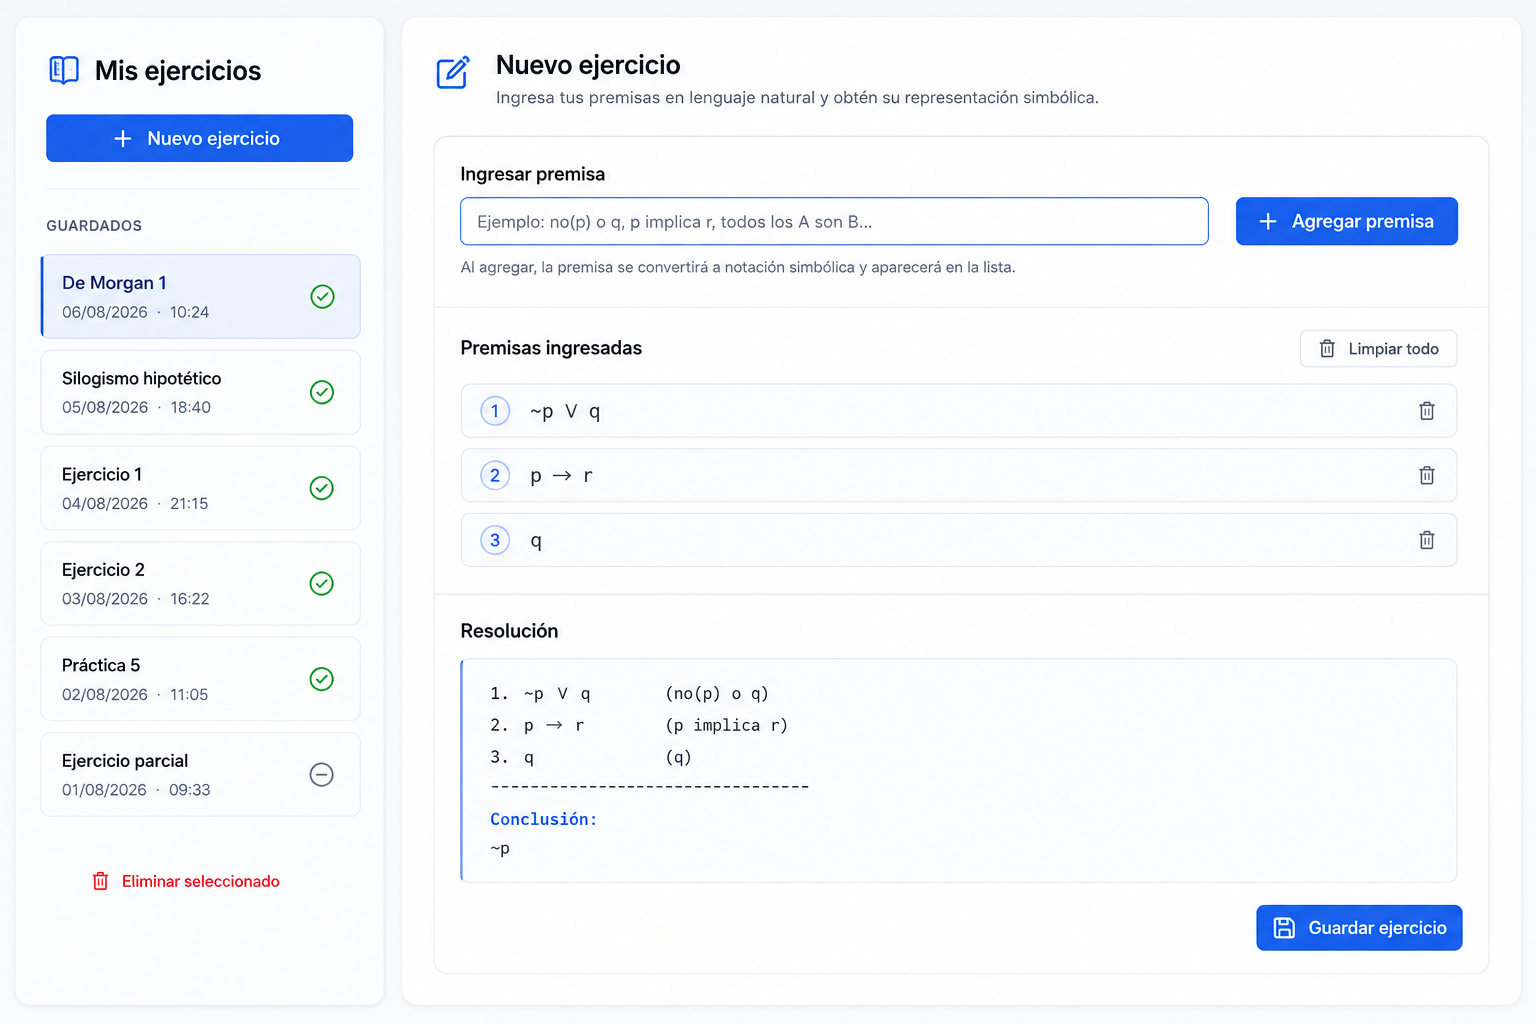
\includegraphics[width=0.85\textwidth]{propuesta_hijos_propuesta-alex.png}
\caption{Boceto del \'arbol sint\'actico (archivo original Hijos de Linus)}
\label{fig:tec-ast}
\end{figure}

\chapter{Motor de cuantificadores}
\label{ch:motor-cuant}
\section{Tokenizador y parser de predicados}
Seis niveles de precedencia con encadenamiento de comparaciones ($a < b < c$ equivale a $(a < b) \land (b < c)$) y potencia con \texttt{Math.pow}. Complejidad $O(n)$.
\section{Dominio $D \subset \mathbb{Z}$}
El dominio acepta listas (\texttt{1, 2, 3}) y rangos (\texttt{0 < x < 9} equivale a $D = \{x \in \mathbb{Z} : 0 < x < 9\}$) con cota de 2000 elementos y deduplicaci\'on. La variante estricta exige solo la variable $x$ y solo enteros.
\begin{figure}[H]
\centering
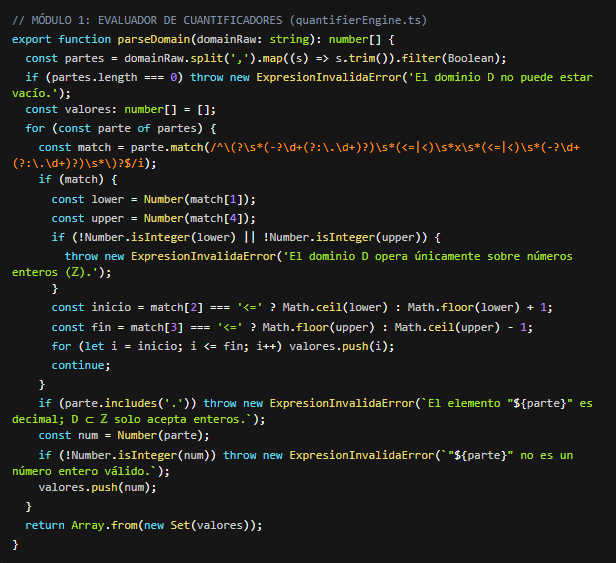
\includegraphics[width=0.9\textwidth]{informe_scratch_modusinnova_p13_616x563_3cb03fed.png}
\caption{Validaci\'on del dominio entero (material original Modus Innova)}
\label{fig:tec-dominio}
\end{figure}
\section{Evaluaci\'on y leyes de reescritura}
Sobre $|D| = m$ elementos el costo es $O(m \cdot n)$ con trazabilidad por elemento, contraejemplo y testigo. El reescritor aplica ocho reglas en orden fijo (doble negaci\'on, $\Delta$, bicondicional, implicaci\'on, De Morgan, distribuci\'on) hasta 15 iteraciones:
\begin{figure}[H]
\centering
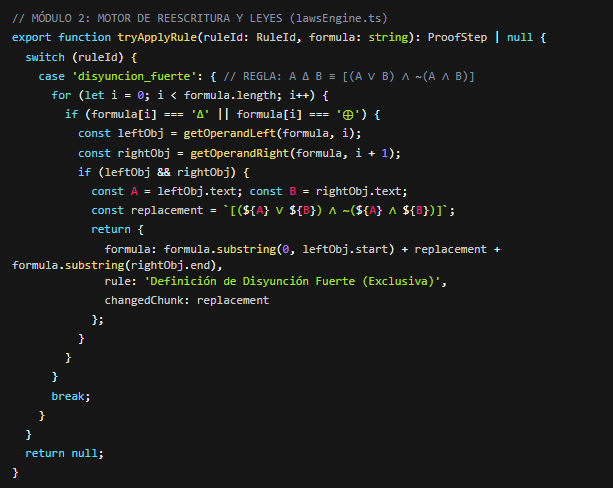
\includegraphics[width=0.9\textwidth]{informe_scratch_modusinnova_p14_613x488_6f3177e1.png}
\caption{Regla de disyunci\'on fuerte (material original Modus Innova)}
\label{fig:tec-delta}
\end{figure}

\chapter{Motor de conjuntos}
\label{ch:motor-conj}
\section{Operaciones puras}
Funciones gen\'ericas sobre conjuntos nativos: uni\'on $O(n+m)$ por propagaci\'on con deduplicaci\'on, resto $O(n)$ por filtrado con pertenencia $O(1)$:
\begin{lstlisting}[language=TypeScript,caption={N\'ucleo de operaciones}]
function union(a, b) { return new Set([...a, ...b]); }
function interseccion(a, b) { return new Set([...a].filter(x => b.has(x))); }
\end{lstlisting}
La potencia usa m\'ascara de bits sobre $2^{n}$ iteraciones ($O(2^{n} \cdot n)$), lo que justifica la advertencia con $|A| > 10$ en la interfaz.
\begin{table}[H]
\centering
\caption{Potencia $P(\{1,2\})$ por m\'ascara binaria}
\begin{tabular}{c|c}
\toprule
M\'ascara & Subconjunto \\
\midrule
00 & $\emptyset$ \\
01 & $\{1\}$ \\
10 & $\{2\}$ \\
11 & $\{1,2\}$ \\
\bottomrule
\end{tabular}
\end{table}
\begin{figure}[H]
\centering
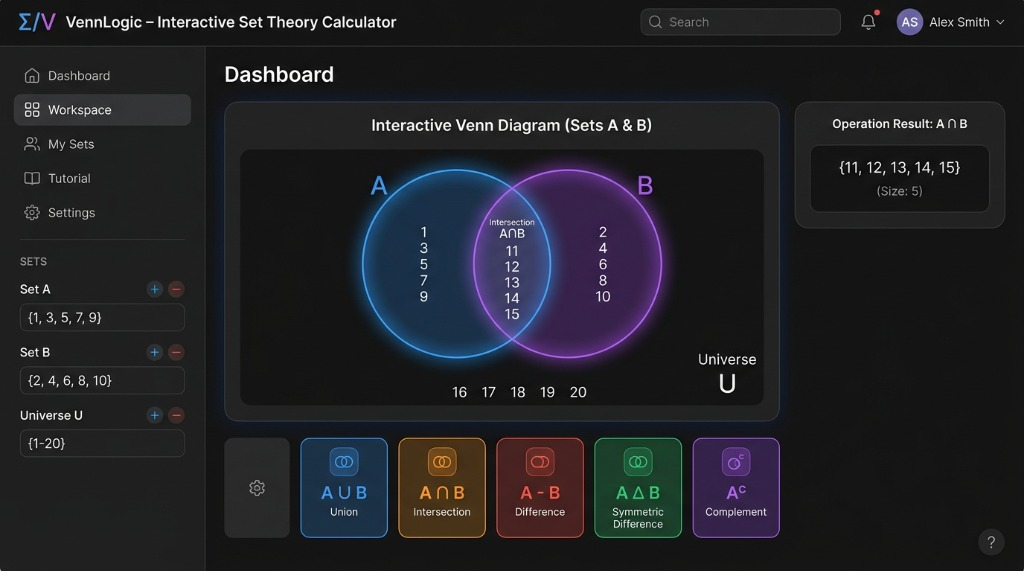
\includegraphics[width=0.9\textwidth]{informe_scratch_linus_p06_1024x571_23455df9.jpeg}
\caption{Diagrama de Venn interactivo (material original Linus)}
\label{fig:tec-venn}
\end{figure}


\chapter{Diez reglas de inferencia en detalle}
\label{ch:reglas-det}
Cada regla indica esquema formal, patr\'on de reconocimiento sobre el \'arbol y ejemplo. Todas son $O(n)$ sobre el tama\~no del \'arbol salvo el dilema ($O(n^{3})$ en b\'usqueda).
\section{Modus Ponens y Modus Tollens}
Modus Ponens: de $p$ y $p \to q$ se deduce $q$. El patr\'on busca una implicaci\'on cuyo antecedente coincida estructuralmente con una premisa. Modus Tollens: de $\lnot q$ y $p \to q$ se deduce $\lnot p$. Ejemplo: con $P \to Q$ y $\lnot Q$ se deriva $\lnot P$.
\section{Silogismos}
El hipot\'etico encadena $p \to q$ y $q \to r$ en $p \to r$ por transitividad. El disyuntivo resuelve $p \lor q$ con $\lnot p$ en $q$. La versi\'on exclusiva opera sobre $\Delta$ con paridad exacta.
\section{Adici\'on, simplificaci\'on y conjunci\'on}
La adici\'on construye $p \lor q$ desde $p$; la simplificaci\'on extrae $p$ desde $p \land q$; la conjunci\'on une dos premisas independientes en $p \land q$.
\section{Doble negaci\'on y dilemas}
La doble negaci\'on cancela $\lnot\lnot p$ en $p$. El dilema constructivo combina $p \to q$, $r \to s$ y $p \lor r$ en $q \lor s$. La eliminaci\'on del bicondicional descompone $p \leftrightarrow q$ en ambos condicionales.
\begin{table}[H]
\centering
\caption{Reglas y costo de reconocimiento}
\begin{tabular}{lll}
\toprule
Regla & Patr\'on & Costo \\
\midrule
Modus Ponens & implicaci\'on + antecedente & $O(n)$ \\
Modus Tollens & implicaci\'on + negaci\'on del consecuente & $O(n)$ \\
Silogismo hipot\'etico & dos implicaciones encadenadas & $O(n)$ \\
Silogismo disyuntivo & disyunci\'on + negaci\'on & $O(n)$ \\
Adici\'on / Simplificaci\'on & construcci\'on / proyecci\'on & $O(n)$ \\
Dilema constructivo & dos implicaciones + disyunci\'on & $O(n^{3})$ \\
\bottomrule
\end{tabular}
\end{table}

\chapter{Diagn\'ostico de falacias con ejemplos}
\label{ch:falacias}
El diagn\'ostico en cascada prioriza: variable ausente, afirmaci\'on del consecuente ($p \to q$, $q \vdash p$ con contraejemplo $p = F$, $q = V$), negaci\'on del antecedente ($p \to q$, $\lnot p \vdash \lnot q$), dilema inverso, contraejemplo general, inconsistencia e incompletitud. Cada diagn\'ostico cita la asignaci\'on que refuta y la regla vulnerada, con valor pedag\'ogico directo.

\chapter{Cat\'alogo de complejidad por funci\'on}
\label{ch:complejidad}
\begin{longtable}{lll}
\caption{Complejidad de las funciones principales} \\
\toprule
Funci\'on & M\'odulo & Complejidad \\
\midrule
\endfirsthead
\caption{Complejidad (continuaci\'on)} \\
\toprule
Funci\'on & M\'odulo & Complejidad \\
\midrule
\endhead
\texttt{union} & conjuntos & $O(n+m)$ \\
\texttt{interseccion} & conjuntos & $O(n)$ \\
\texttt{diferencia} & conjuntos & $O(n)$ \\
\texttt{potencia} & conjuntos & $O(2^{n} \cdot n)$ \\
\texttt{normalizar} & tablas & $O(n)$ \\
\texttt{tokenizar} & tablas & $O(n)$ \\
\texttt{parsear*} (5 niveles) & tablas & $O(n)$ \\
\texttt{evaluar} & tablas & $O(\text{nodos})$ \\
\texttt{generarFilas} & tablas & $O(2^{v} \cdot n)$ \\
\texttt{encontrarContraejemplo} & inferencias & $O(2^{v} \cdot p \cdot n)$ \\
\texttt{demostrarConclusion} & inferencias & $O(12 \cdot (n + n^{2} + n^{3}))$ \\
\texttt{tokenizeExpression} & cuantificadores & $O(n)$ \\
\texttt{parseDomain} & cuantificadores & $O(n)$ \\
\texttt{evaluarCuantificador} & cuantificadores & $O(m \cdot n)$ \\
\texttt{solveFormula} & leyes & $O(15 \cdot r \cdot n)$ \\
\bottomrule
\end{longtable}
Los l\'imites expl\'icitos (2000 elementos de dominio, 12 iteraciones, advertencia con $|A| > 10$) evitan la explosi\'on combinatoria.

\chapter{Comparaci\'on de los dos parsers}
\label{ch:parsers}
El parser de tablas usa esc\'aner por caracteres con s\'imbolos Unicode y cinco niveles; el del solver usa esc\'aner por palabras con espa\~nol formal y cuatro niveles. Ambos son descendentes recursivos $O(n)$ con recursi\'on derecha para la negaci\'on.
\begin{table}[H]
\centering
\caption{Gram\'aticas comparadas}
\begin{tabular}{ll}
\toprule
Tablas & Solver \\
\midrule
Iff $\leftrightarrow$ & Implicaci\'on y bicondicional \\
Implies $\to$ & Disyunciones \\
Or $\lor$ & Conjunci\'on $Y$ \\
And $\land$ & Negaci\'on $NO$ \\
Not $\lnot$ & Primario \\
Primario & --- \\
\bottomrule
\end{tabular}
\end{table}


\chapter{Diario de sprints por equipo}
\label{ch:diario}
\section{Sprint 1 --- Propuesta}
Cada equipo entreg\'o wireframes y decisi\'on de pila: Sinergia propuso el motor proposicional con precedencia cl\'asica; Hijos de Linus el demostrador con trazabilidad; Modus Innova el evaluador sobre $D \subset \mathbb{Z}$ con $\Delta$; Linus la calculadora con Venn. La plantilla base Vue 3 + Vite se cre\'o con la estructura que se mantuvo todo el desarrollo.
\begin{figure}[H]
\centering
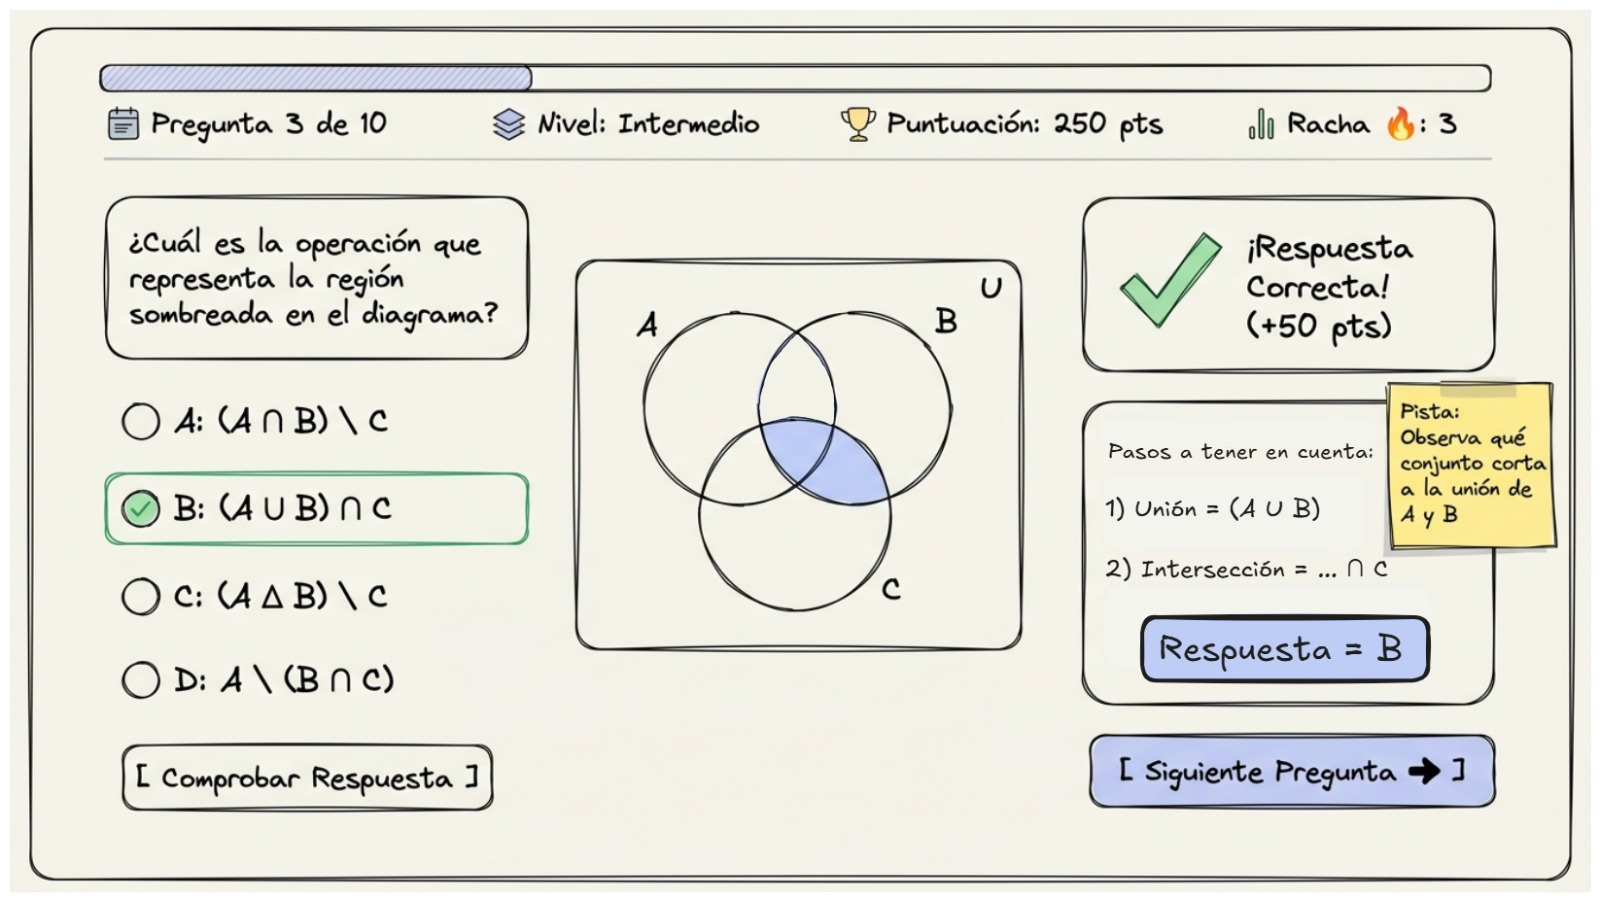
\includegraphics[width=0.48\textwidth]{propuesta_linus_propuesta-fernando.jpg}
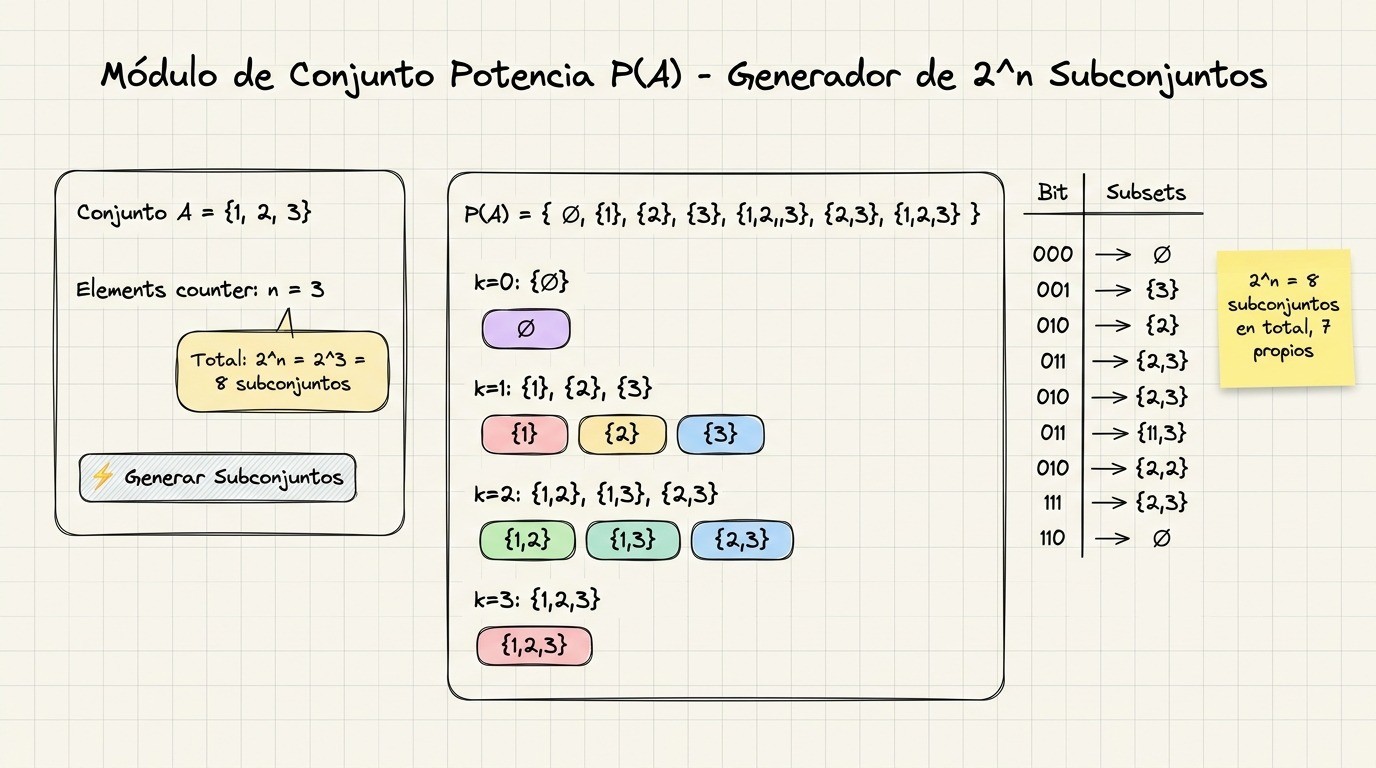
\includegraphics[width=0.48\textwidth]{propuesta_linus_propuesta-mike.jpg}
\caption{Propuestas Fernando y Mike (Linus, archivos originales)}
\label{fig:tec-diario1}
\end{figure}
\section{Sprint 2 --- Motores}
Se implementaron los motores en TypeScript puro con pruebas iniciales: el evaluador con 15 pruebas, el solver con tipos y primera regla, el parser l\'exico-sint\'actico de conjuntos y el h\'ibrido de cuantificadores con cota de 2000 elementos.
\begin{figure}[H]
\centering

\includegraphics[width=0.9\textwidth]{informe_scratch_sinergia_p11_1142x473_443fddb8.png}
\caption{Parser del equipo Sinergia, detalle (material original)}
\label{fig:tec-diario2}
\end{figure}
\section{Sprint 3 --- Interfaz}
Se desarrollaron las vistas Vue con diagrama SVG, trazabilidad, tablas de verdad y cat\'alogo de leyes, con componentes compartidos de botones, tarjetas e insignias y marca azul com\'un.
\begin{figure}[H]
\centering
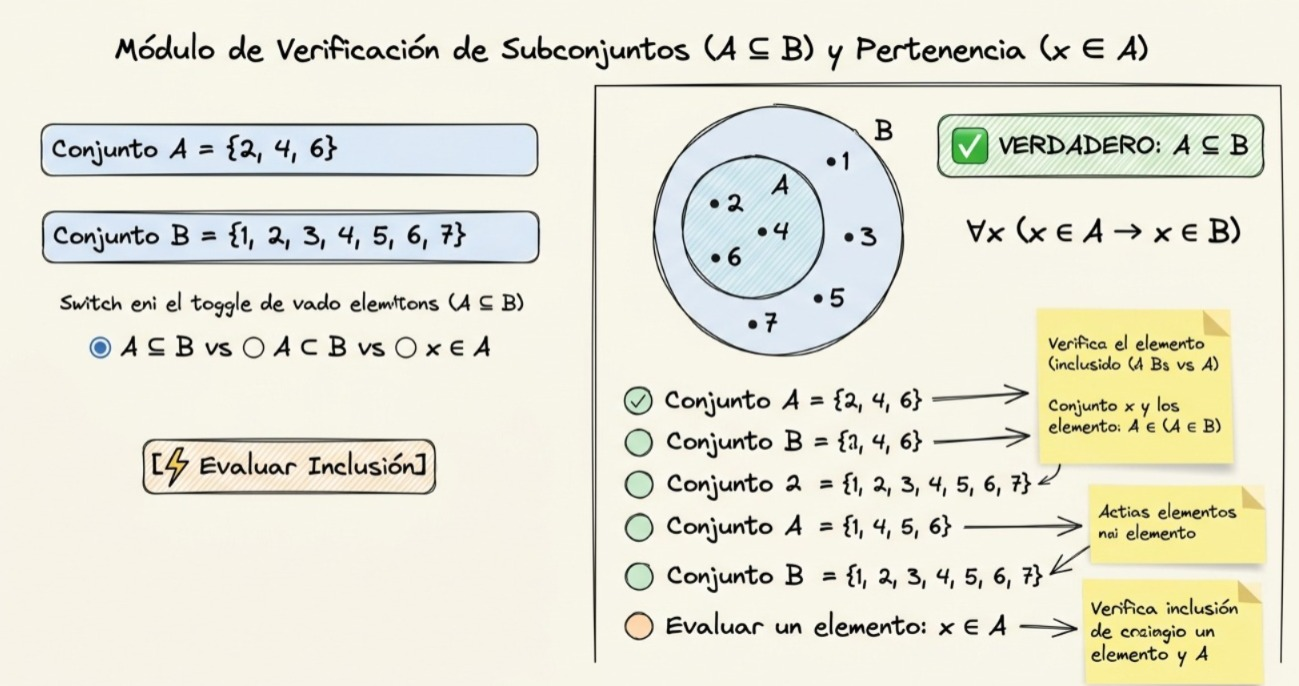
\includegraphics[width=0.48\textwidth]{propuesta_linus_propuesta-nio.jpg}
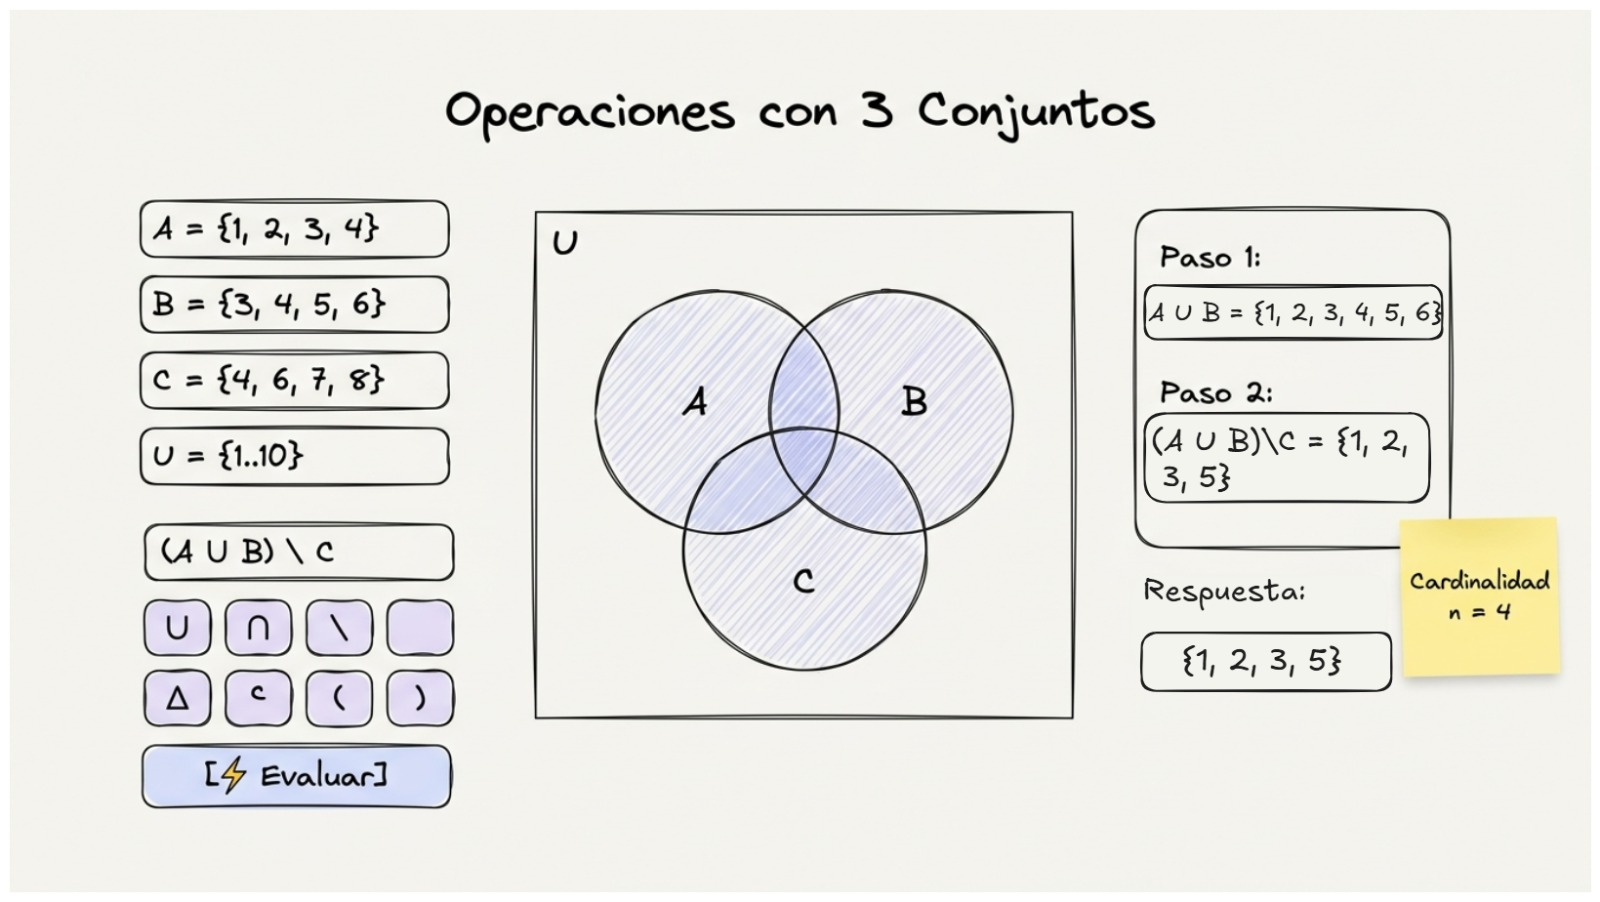
\includegraphics[width=0.48\textwidth]{propuesta_linus_propuesta-sergio.jpg}
\caption{Propuestas Nio y Sergio (Linus, archivos originales)}
\label{fig:tec-diario3}
\end{figure}
\section{Sprint 4 --- Refinamiento y calidad}
Se incorporaron mejoras solicitadas (par\'entesis, cuadros estad\'isticos, sub-selector de potencia, correcci\'on del complemento y del SVG, normalizaci\'on de textos), se alcanzaron 189 pruebas y se document\'o el despliegue.
\begin{figure}[H]
\centering
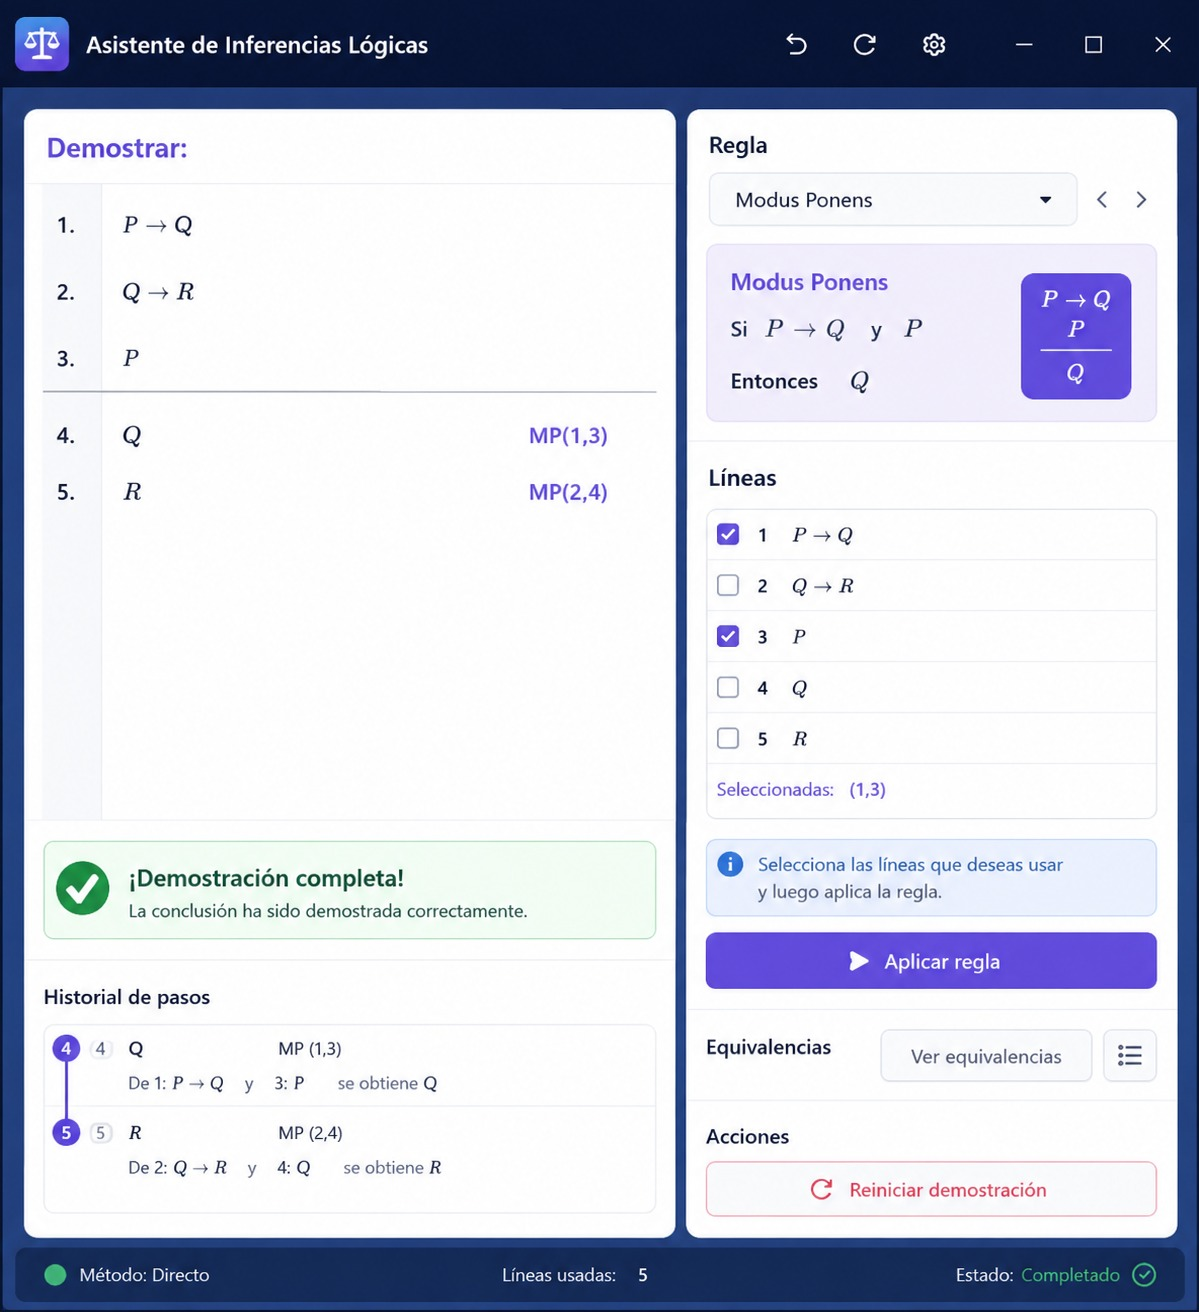
\includegraphics[width=0.85\textwidth]{propuesta_hijos_propuesta-morocho.jpeg}
\caption{Entorno de pr\'actica del equipo Hijos de Linus (archivo original)}
\label{fig:tec-diario4}
\end{figure}

\chapter{Cat\'alogo de pruebas por archivo}
\label{ch:tests}
\begin{longtable}{ll}
\caption{Archivos de prueba y cobertura} \\
\toprule
Archivo & Cubre \\
\midrule
\endfirsthead
\caption{Pruebas (continuaci\'on)} \\
\toprule
Archivo & Cubre \\
\midrule
\endhead
\texttt{evaluator.test.ts} & Parser, evaluador y clasificaci\'on de tablas \\
\texttt{parser.test.ts} & Precedencia y errores del solver \\
\texttt{solver.test.ts} & Diez reglas y contraejemplos \\
\texttt{astVisual.test.ts} & Serializaci\'on del \'arbol \\
\texttt{engine.test.ts} & Tokenizador y dominios de cuantificadores \\
\texttt{operations.test.ts} & Uni\'on, intersecci\'on, potencia (14 casos) \\
\texttt{trazabilidad.test.ts} & Historial con 9 pruebas y 22 aserciones \\
\texttt{validator.test.ts} & Sanitizaci\'on con 27 pruebas \\
\texttt{validator\_stress.test.ts} & Inyecciones y anidaci\'on (15 pruebas) \\
\texttt{integracion\_motor.test.ts} & Tuber\'ia completa sanitizaci\'on-demostraci\'on \\
\texttt{ArbolAST.test.ts} & Render del \'arbol \\
\texttt{FormularioInferencia.test.ts} & Entrada de premisas \\
\texttt{IndicadorResultado.test.ts} & Estados v\'alida/inv\'alida \\
\texttt{PanelTrazabilidad.test.ts} & Pasos y exportaci\'on \\
\texttt{TraductorLenguajeNatural.test.ts} & Mapas de variables \\
\texttt{index.test.ts} & Integraci\'on de la p\'agina \\
\texttt{test\_ejemplo.test.ts} & Ejemplo m\'inimo \\
\bottomrule
\end{longtable}
La matriz de casos borde del validador cubre entradas vac\'ias, caracteres prohibidos, emojis, inyecciones, operadores en m\'ultiples notaciones, par\'entesis anidados y desbalanceados, y operadores consecutivos.

\chapter{Leyes formales con demostraci\'on esquem\'atica}
\label{ch:leyes-formal}
Idempotencia, asociativa y conmutativa se prueban por inspecci\'on de 4 filas. La distributiva requiere 8 filas. Morgan se prueba mostrando el intercambio $\land \leftrightarrow \lor$ fila a fila. La absorci\'on se reduce por casos en $p$. La identidad se lee directo de las constantes. La expansi\'on usa que $q \lor \lnot q$ es tautolog\'ia. La contraposici\'on comparte tabla con el condicional. La exportaci\'on anida condicionales. La definici\'on traduce $\to$ y $\leftrightarrow$ a $\lnot$, $\lor$ y $\land$.
\begin{figure}[H]
\centering
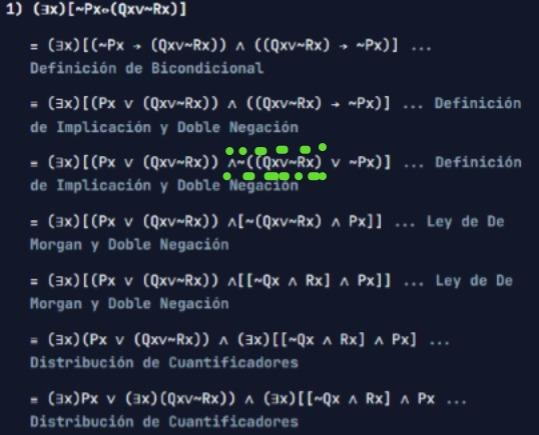
\includegraphics[width=0.9\textwidth]{informe_scratch_modusinnova_p09_539x435_0b0dfc19.jpeg}
\caption{Demostraci\'on paso a paso del motor de leyes (Modus Innova, material original)}
\label{fig:tec-leyes-demo}
\end{figure}

\chapter{M\'odulos de validaci\'on, trazabilidad y transcripci\'on}
\label{ch:val-traz}
El validador normaliza m\'as de 15 notaciones ($\to$, $\land$, \texttt{->}, \texttt{\&\&}, palabras) hacia claves can\'onicas, previene inyecciones y valida par\'entesis para formularios reactivos. La trazabilidad acumula pasos en orden con instant\'aneas de estado y reexporta tipos y funciones. La transcripci\'on mapea cada regla a nombre, alias y descripci\'on general, arma oraciones citando l\'ineas y renderiza el \'arbol a texto legible.

\chapter{P\'aginas Vue y sistema de contenido}
\label{ch:pages}
Las nueve vistas orquestan entradas reactivas, motores y contenido sin contener l\'ogica: Tablas detecta variables en vivo; Conjuntos computa regiones y colores del Venn; Inferencias procesa en as\'incrono con historial local; Cuantificadores eval\'ua en dual y resuelve leyes; Inicio, Aprender, Leyes y Progreso componen hero, recorrido de cuatro pasos, b\'usqueda y gr\'afico de precisi\'on. El contenido visible proviene de claves por m\'odulo con interruptor de modo literal.
\begin{figure}[H]
\centering

\includegraphics[width=0.9\textwidth]{informe_scratch_sinergia_p17_1142x458_12b2a8af.png}
\caption{Propiedades computadas de la vista (material original Sinergia)}
\label{fig:tec-computed}
\end{figure}

\chapter{Integraci\'on Vue y contenido externalizado}
\label{ch:vue}
Cada p\'agina orquesta entradas reactivas, motores y contenido: la entrada se parsea, se detectan variables en vivo, se generan filas y se clasifica; los errores de parseo se muestran sin romper la vista. El contenido visible proviene de claves por m\'odulo con interruptor de modo literal que elige s\'imbolos o palabras. La correspondencia pantalla-contenido se resume en la Tabla~\ref{tab:traz}.
\begin{table}[H]
\centering
\caption{Trazabilidad pantalla-contenido (selecci\'on)}
\begin{tabular}{ll}
\toprule
Elemento & Clave \\
\midrule
Tablas: variables y conectores & \texttt{tablas.info} \\
Cuantificadores: dominio y predicado & \texttt{cuantificadores.dominio, .predicado} \\
Inferencias: trazabilidad & \texttt{inferencias.trazabilidad} \\
Conjuntos: operaciones y Venn & \texttt{conjuntos.operaciones, .diagrama} \\
\bottomrule
\end{tabular}
\label{tab:traz}
\end{table}
\begin{figure}[H]
\centering

\includegraphics[width=0.9\textwidth]{informe_scratch_sinergia_p16_1142x1085_8070cdb1.png}
\caption{Estado reactivo de la vista de tablas (material original Sinergia)}
\label{fig:tec-estado}
\end{figure}

\chapter{Pruebas, calidad y despliegue}
\label{ch:pruebas}
La suite suma 189 pruebas en 17 archivos que validan parsers, evaluadores, leyes y componentes, con verificaci\'on de tipos estricta y compilaci\'on de producci\'on. El despliegue publica la compilaci\'on en GitHub Pages con redirecci\'on para rutas y vistas previas por Pull Request.
\begin{figure}[H]
\centering

\includegraphics[width=0.9\textwidth]{informe_scratch_sinergia_p25_1139x326_547a68c9.png}
\caption{Cronograma de sprints (material original Sinergia)}
\label{fig:tec-cron}
\end{figure}

\chapter{Evoluci\'on por sprints}
\label{ch:sprints}
Propuesta con wireframes y decisi\'on de Vue 3; motores con pruebas iniciales; interfaz con componentes compartidos y diagramas; calidad con 189 pruebas y documentaci\'on. Los bocetos originales se conservan como evidencia.
\begin{figure}[H]
\centering
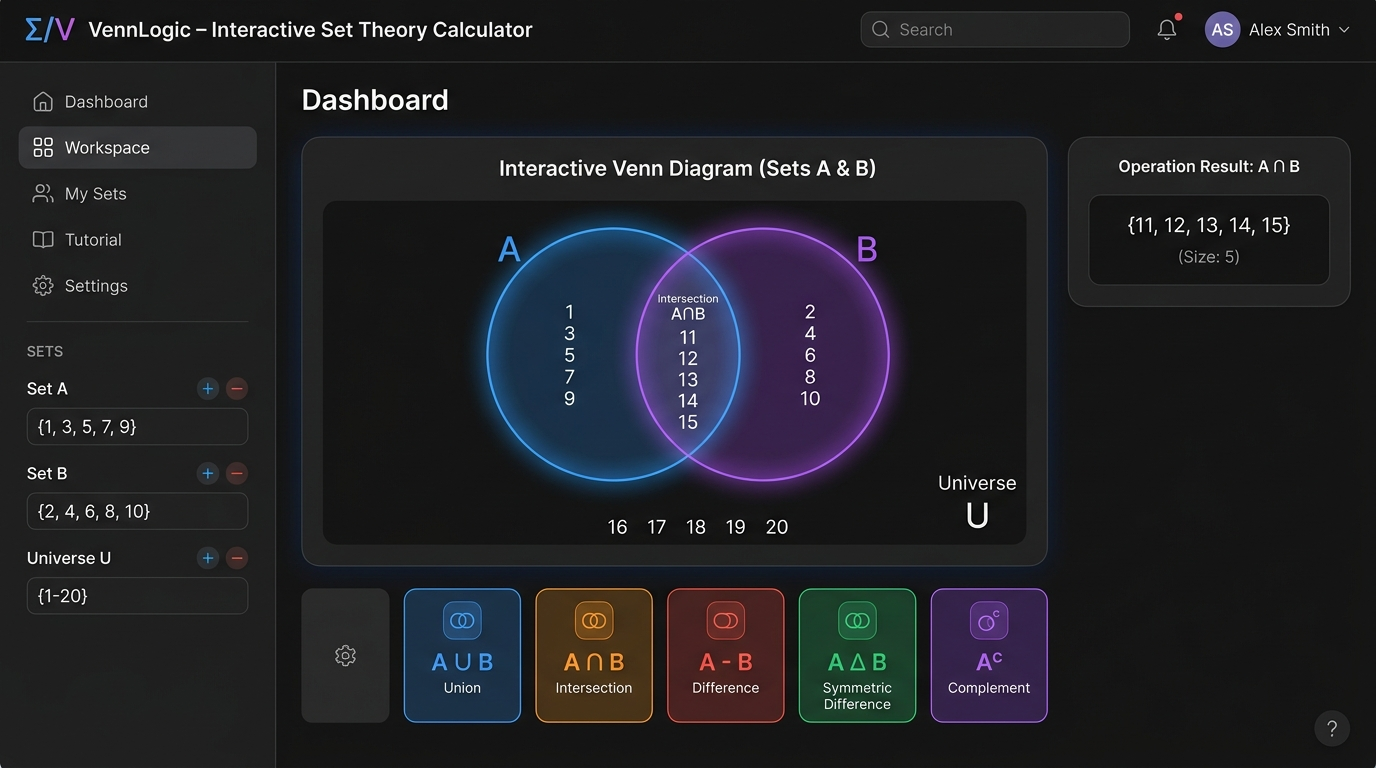
\includegraphics[width=0.48\textwidth]{propuesta_linus_propuesta-jordy.jpg}
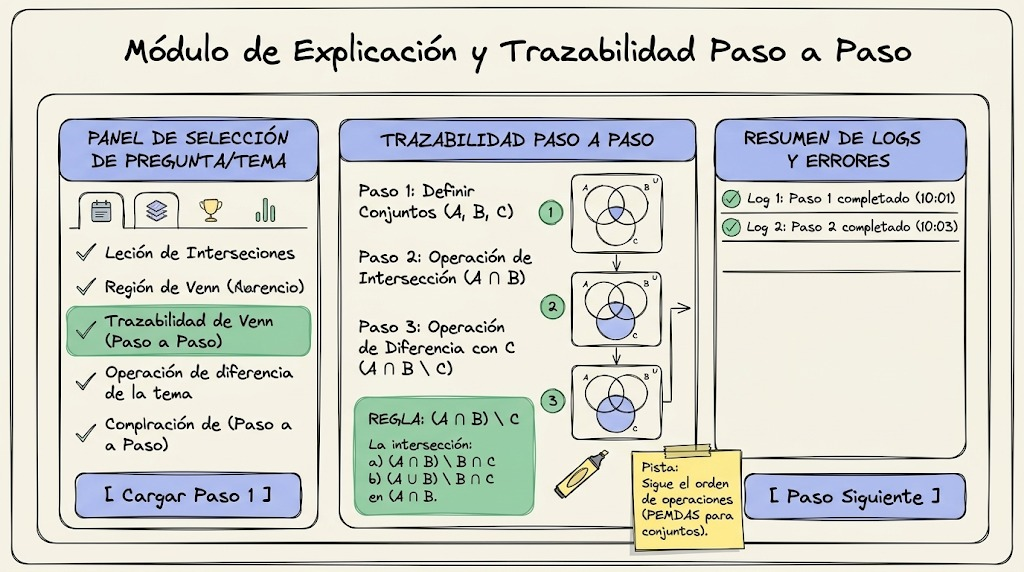
\includegraphics[width=0.48\textwidth]{propuesta_linus_propuesta-alejandro.jpg}
\caption{Bocetos del equipo Linus (archivos originales)}
\label{fig:tec-linus-boc}
\end{figure}
\begin{figure}[H]
\centering
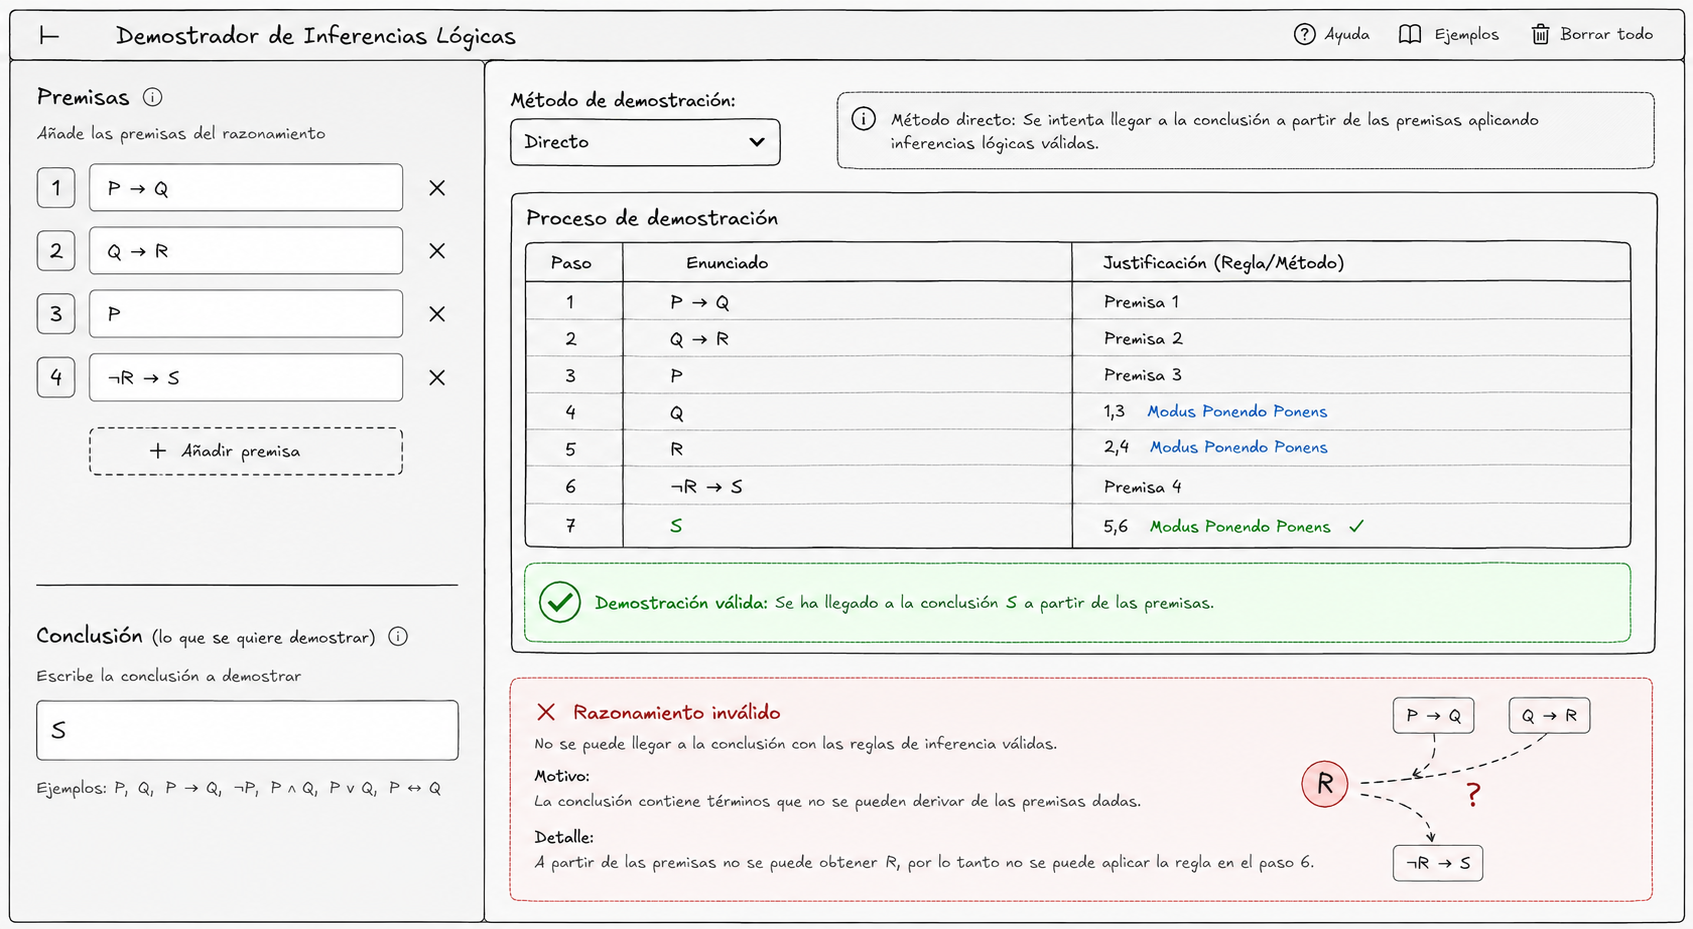
\includegraphics[width=0.85\textwidth]{propuesta_hijos_propuesta-arnold.png}
\caption{Interfaz del equipo Hijos de Linus (archivo original)}
\label{fig:tec-hijos-ui}
\end{figure}

\chapter{Conclusiones}
\label{ch:concl}
La separaci\'on entre motores y vistas permiti\'o colaborar sin colisiones y editar contenido docente sin c\'odigo. Los l\'imites expl\'icitos ($2^{v}$ filas, 2000 elementos de dominio, 12 iteraciones de encadenamiento) muestran conciencia de complejidad. El trabajo futuro incluye exportaci\'on de tablas, calificaci\'on y l\'ogica de primer orden completa.
















\chapter{Anexo: bit\'acoras de sprint (transcripci\'on fiel formateada)}
\label{ch:anexo-sprints}
Este anexo transcribe fielmente las bit'acoras registradas por los equipos en 	exttt{TAREAS/}, convertidas de Markdown a \LaTeX\ con ortograf'ia corregida y terminolog'ia unificada ($D \subset \mathbb{Z}$, conectivos $\lnot$, $\land$, $\lor$, $	o$, $\leftrightarrow$). Constituyen la evidencia de trabajo por sprints.

\section{Propuesta Sinergia}
\textit{Fuente original: \texttt{../TAREAS/01\_Propuesta/sinergia/propuesta.md}}

\section{LogiLearn}

\textbf{Equipo:} Sinergia

\textbf{Integrantes:}
\begin{itemize}[leftmargin=*]
\item Julio Miguel Velarde Avila
\item Segundo Jesús Nuñez Esquen
\item Aldair Wilfredo Querevalu Esquen
\item Luis Smith Atencio Fiestas
\item Alexa Jhosely Benavides Irigoin (líder)
\end{itemize}

\textbf{Tema:} Tablas de verdad y leyes lógicas

\subsubsection{1. Problema a Resolver}
El aprendizaje de la lógica simbólica puede resultar complicado para los estudiantes debido a la dificultad para comprender y aplicar conceptos como proposiciones, conectores lógicos, tablas de verdad y leyes lógicas.
Además, el aprendizaje exclusivamente teórico puede dificultar la práctica y la identificación de errores durante la resolución de ejercicios.

\subsubsection{2. Funcionalidad Propuesta}
Se propone desarrollar una plataforma web interactiva  que facilite el aprendizaje de la lógica simbólica mediante explicaciones, ejemplos y ejercicios prácticos.
La herramienta permitirá al estudiante practicar los principales conceptos de lógica simbólica y recibir una retroalimentación que facilite su aprendizaje.
LogiLearn es una plataforma web interactiva para aprender lógica proposicional de forma visual. Incluye:

\begin{itemize}[leftmargin=*]
\item \textbf{Página de inicio:} presenta la herramienta y sus módulos principales (Tablas de verdad, Leyes lógicas, Ejercicios prácticos y Tu progreso), con acceso mediante inicio de sesión.
\item \textbf{Módulo de Tablas de Verdad:} permite ingresar una proposición lógica (usando variables p, q, r y operadores como Y, O, NO), generar automáticamente su tabla de verdad y visualizar el resultado de la expresión evaluada.
\item \textbf{Módulo de Leyes Lógicas:} muestra de forma didáctica las distintas leyes lógicas (De Morgan, Distributiva, entre otras) organizadas en tarjetas visuales, facilitando su comprensión y repaso.
\item \textbf{Seguimiento de progreso:} el sistema permite al usuario continuar su aprendizaje desde donde lo dejó, guardando su avance en los módulos.
\end{itemize}

\subsubsection{3. Boceto Visual (Wireframe)}
Diseño elaborado en Figma:
 Ver diseño en Figma (\url{https://www.figma.com/design/MRiWbcWmQAohkH3CqKPGeb/Interfaz-Web---Inicio?node-id=81-3&t=iMJkIZVvPtwiNntF-1})

<img width='1446' height='13186' alt='Interfaz Web - Inicio (1)' src='https://github.com/user-attachments/assets/afc3e676-fb55-4c4c-a768-c5f18a70b53f' />


\section{Propuesta Hijos de Linus}
\textit{Fuente original: \texttt{../TAREAS/01\_Propuesta/hijos-de-linus/propuesta.md}}

\section{Asistente e Intérprete de Inferencias Lógicas}

\textbf{Equipo:} Los Hijos de Linus
\textbf{Integrantes:} Espinoza Arom, Centurión Alex, Mio Arnold, Morocho Juan, Altamirano Renatto
\textbf{Tema:} Inferencias Lógicas

\hrulefill

\subsubsection{1. Problema a Resolver}

El aprendizaje de las inferencias lógicas en estudiantes universitarios presenta dos dificultades principales:
1. \textbf{Dificultad en la resolución asistida y verificación:} A los estudiantes les cuesta comprobar de forma rápida si un razonamiento lógico es válido o inválido, así como visualizar la demostración formal mediante método directo o indirecto.
2. \textbf{Dificultad en el aprendizaje interactivo paso a paso:} Muchos estudiantes tienen problemas para identificar y aplicar correctamente las reglas de inferencia por sí mismos en el desarrollo de una prueba, cometiendo errores de deducción sin recibir retroalimentación inmediata sobre qué falla en su razonamiento.

\hrulefill

\subsubsection{2. Funcionalidad Propuesta}

La herramienta consistirá en un sistema web interactivo compuesto por \textbf{dos interfases (módulos) principales}:

\paragraph{2.1. Interfaz de Calcular y Resolver (Resolución Automática)}
\begin{itemize}[leftmargin=*]
\item \textbf{Ingreso de Datos:} El usuario ingresa un conjunto de premisas y la conclusión que se desea demostrar.
\item \textbf{Selección de Método:} Permite elegir entre el \textbf{Método Directo} o el \textbf{Método Indirecto} (Reducción al absurdo).
\item \textbf{Motor de Resolución:} El sistema reescribe las premisas utilizando equivalencias lógicas según sea conveniente y genera la demostración completa del razonamiento de manera automática.
\end{itemize}

\paragraph{2.2. Interfaz de Practicar Ejercicios (Resolución Guiada e Interactiva)}
\begin{itemize}[leftmargin=*]
\item \textbf{Entorno de Práctica:} El estudiante inicia con las premisas y la conclusión del ejercicio a resolver.
\item \textbf{Aplicación Manual de Reglas:} El usuario selecciona manualmente una regla de inferencia y especifica sobre qué líneas de premisas desea aplicarla.
\item \textbf{Validación en Tiempo Real:}
\item Si la aplicación es \textbf{correcta}, el sistema agrega automáticamente la nueva proposición derivada y habilita el siguiente paso.
\item Si la aplicación es \textbf{incorrecta}, la plataforma muestra un mensaje de retroalimentación indicando el error cometido.
\item \textbf{Objetivo:} Acompañar el proceso de aprendizaje permitiendo al estudiante construir la demostración paso a paso hasta llegar a la conclusión.
\end{itemize}

\hrulefill

\subsubsection{3. Boceto Visual (Wireframe)}

\paragraph{Módulo 1: Interfaz de Calcular y Resolver}
!Interfaz de Calcular y Resolver (\url{assets/propuesta-arnold.png})

\paragraph{Módulo 2: Interfaz de Practicar Ejercicios}
!Interfaz de Practicar Ejercicios (\url{assets/propuesta-morocho.jpeg})

\hrulefill

\subsubsection{Observación}

La herramienta busca integrar tanto un componente utilitario de resolución automatizada como un componente pedagógico interactivo. Para un desarrollo eficiente, la plataforma dispondrá de un módulo centralizado de equivalencias y reglas de inferencia lógicas reutilizable en ambos sistemas.


\section{Propuesta Linus}
\textit{Fuente original: \texttt{../TAREAS/01\_Propuesta/linus/propuesta.md}}

\section{Asistente e Intérprete de Teoría de Conjuntos y Diagramas de Venn}

\textbf{Equipo:} Equipo Linus
\textbf{Integrantes:} Jordy (Sublíder), Junior, Mike, Sergio, Fernando, Alejandro
\textbf{Tema:} Teoría de Conjuntos y Diagramas

\hrulefill

\subsubsection{1. Problema a Resolver}

El aprendizaje de la Teoría de Conjuntos y los Diagramas de Venn en estudiantes universitarios presenta dos dificultades principales:
1. \textbf{Dificultad en la visualización espacial y cálculo de operaciones:} A los estudiantes les cuesta comprobar de forma rápida si una operación entre dos o tres conjuntos produce el resultado correcto y qué elementos exactos pertenecen a cada región del diagrama.
2. \textbf{Dificultad en el cálculo del Conjunto Potencia y relaciones de pertenencia/inclusión:} Muchos estudiantes confunden pertenencia con inclusión y tienen problemas para listar manualmente todos los subconjuntos.

\hrulefill

\subsubsection{2. Funcionalidad Propuesta}

La herramienta consistirá en un sistema web interactivo compuesto por \textbf{dos módulos principales}:

\paragraph{2.1. Calculadora de Conjuntos y Diagrama de Venn}
\begin{itemize}[leftmargin=*]
\item El usuario ingresa un Universo U y los conjuntos A, B y opcionalmente C.
\item Permite elegir entre Unión, Intersección, Diferencia, Diferencia Simétrica, Complemento o Conjunto Potencia.
\item Genera el Diagrama de Venn iluminando en tiempo real la región correspondiente.
\end{itemize}

\paragraph{2.2. Evaluador de Propiedades y Práctica Guiada}
\begin{itemize}[leftmargin=*]
\item Comprueba automáticamente si A $ \subseteq $ B, si A = B, o si son disjuntos.
\item Genera todos los subconjuntos del Conjunto Potencia con explicación paso a paso.
\item Permite a los estudiantes validar sus ejercicios de forma inmediata.
\end{itemize}

\hrulefill

\subsubsection{3. Boceto Visual (Wireframe)}

\paragraph{Módulo de Calculadora e Interfaz de Venn (Jordy)}
!Boceto de Jordy (\url{assets/propuesta-jordy.jpg})

\paragraph{Módulo de Verificación de Subconjuntos (Junior)}
!Boceto de Junior (\url{assets/propuesta-junior.jpg})

\paragraph{Módulo de Conjunto Potencia (Mike)}
!Boceto de Mike (\url{assets/propuesta-mike.jpg})

\paragraph{Módulo de Operaciones con 3 Conjuntos (Sergio)}
!Boceto de Sergio (\url{assets/propuesta-sergio.jpg})

\paragraph{Módulo de Ejercicios Didácticos (Fernando)}
!Boceto de Fernando (\url{assets/propuesta-fernando.jpg})

\paragraph{Módulo de Explicación Paso a Paso (Alejandro)}
!Boceto de Alejandro (\url{assets/propuesta-alejandro.jpg})

\hrulefill

\subsubsection{Observación}

La herramienta busca integrar un módulo de resolución y graficación de Venn con un componente didáctico de verificación de propiedades para fortalecer los conceptos de Teoría de Conjuntos.

\section{Propuesta Modus Innova}
\textit{Fuente original: \texttt{../TAREAS/01\_Propuesta/modus-innova/propuesta.md}}

\section{Validador y Tutor Interactivo de Cuantificadores y Silogismos Lógicos (QuantifiWeb)}

\textbf{Equipo:} Equipo 4 --- Modus Innova (QuantifiTech)
\textbf{Integrantes:} Cristian (Sublíder), Danuska, Marlon, Guillermo, Noemí
\textbf{Tema Asignado:} Cuantificadores Lógicos, Lógica de Predicados y Silogismos / Inferencias

\hrulefill

\subsubsection{1. Descripción del Problema}
En el aprendizaje de la Lógica Simbólica y Predicados, a los estudiantes universitarios les resulta especialmente difícil enfrentarse a dos conceptos fundamentales:

1. \textbf{Cuantificadores Lógicos ($\forall$ Universal y $\exists$ Existencial):}
   A los alumnos les cuesta evaluar el valor de verdad ($\text{Verdadero}$ o $\text{Falso}$) de proposiciones cuantificadas sobre un \textbf{Dominio de Discurso} finito (ej. $D = \{1, 2, 3, 4, 5\}$). Además, suelen confundirse al aplicar las \textbf{Leyes de Negación de Cuantificadores (De Morgan)}:
   $$\neg (\forall x P(x)) \equiv \exists x \neg P(x)$$
   $$\neg (\exists x P(x)) \equiv \forall x \neg P(x)$$
   y en comprender cómo un solo elemento en el dominio puede actuar como contraejemplo que invalide una afirmación universal.

2. \textbf{Inferencias Lógicas y Silogismos:}
   Les resulta difícil identificar si un argumento (compuesto por varias premisas y una conclusión) es \textbf{formalmente válido o es una falacia}. Asimismo, al intentar resolver ejercicios manuscritos, frecuentemente se confunden sobre \textbf{qué Regla de Inferencia aplicar} (\textit{Modus Ponens}, \textit{Modus Tollens}, \textit{Silogismo Hipotético}, \textit{Silogismo Disyuntivo}) y cómo justificar cada paso formal para llegar a la conclusión.

\hrulefill

\subsubsection{2. ¿Qué hará nuestro componente?}
Nuestra herramienta web \textbf{QuantifiWeb} será una interfaz visual interactiva que integrará dos módulos funcionales explicativos y aplicativos en tiempo real:

1. \textbf{Módulo de Cuantificadores Lógicos (Lógica de Predicados):}
\begin{itemize}[leftmargin=*]
\item \textbf{Definición de Dominio y Predicados (Inputs):} El usuario ingresa un conjunto universo $D$ (ej. \texttt{1, 2, 3, 4, 5}) y la condición de su predicado $P(x)$ (ej. \texttt{'x es par'}).
\item \textbf{Evaluación en Dominio con Trazabilidad:} Al presionar \textbf{' Evaluar Cuantificador'}, el sistema evalúa la fórmula elemento por elemento dentro del dominio $D$, mostrando la tabla de trazabilidad ($P(1)=\text{F}$, $P(2)=\text{V}$, etc.), el resultado global ( \textbf{VERDADERO} o  \textbf{FALSO}) y el contraejemplo o caso de éxito.
\item \textbf{Asistente de Negación (De Morgan):} Botón \textbf{' Negar Expresión'} que calcula automáticamente la proposición equivalente con el cuantificador opuesto y su negación interna.
\end{itemize}

2. \textbf{Módulo de Inferencias Lógicas y Silogismos:}
\begin{itemize}[leftmargin=*]
\item \textbf{Ingreso del Argumento (Inputs):} El usuario verá dos cajas de texto principales para ingresar la \textbf{Premisa 1} (ej. \texttt{p  q}) y la \textbf{Premisa 2} (ej. \texttt{p}), además de una caja de texto para la \textbf{Conclusión} (ej. \texttt{q}).
\item \textbf{Barra de Teclado Rápido de Símbolos:} Contará con una barra de \textbf{botones rápidos de símbolos lógicos} (\texttt{}, \texttt{}, \texttt{}, \texttt{}, \texttt{}, \texttt{}, \texttt{}, \texttt{}) para facilitar la escritura sin cometer errores de tipeo.
\item \textbf{Verificación e Interacción Paso a Paso:} Al hacer clic en el botón \textbf{' Validar Inferencia'}:
\item \textbf{Si la inferencia es VÁLIDA:} El panel se iluminará en verde, mostrará un mensaje destacado como \texttt{ Argumento Valido!} y desplegará la explicación paso a paso indicando la regla exacta utilizada (ej. \textit{'Se aplicó la regla Modus Ponens [MP] a partir de la Premisa 1 y Premisa 2'}).
\item \textbf{Si la inferencia es INVÁLIDA (Falacia):} El panel se pondrá de color rojo alertando \texttt{ Argumento Invalido (Falacia)}, y mostrará un ejemplo de la vida real (contraejemplo) explicando por qué las premisas no garantizan esa conclusión.
\end{itemize}

3. \textbf{Modo Didáctico de Práctica ('Cargar Ejemplo'):}
\begin{itemize}[leftmargin=*]
\item Incluirá un botón de \textbf{' Cargar Ejemplo'} para que los alumnos que no tengan ejercicios a la mano puedan probar casos preescritos de Modus Ponens, Modus Tollens, Silogismos y Cuantificadores.
\end{itemize}

\hrulefill

\subsubsection{3. Boceto Visual (Wireframe)}

A continuación se presenta la distribución estructurada de pantallas, componentes, entradas y paneles de resultado de la herramienta:

\begin{lstlisting}[language={},basicstyle=\ttfamily\scriptsize]
+-----------------------------------------------------------------------------------+
|   LOGICA SIMBOLICA GLOBAL  |  Equipo 3: Modus Innova -- QuantifiWeb             |
+-----------------------------------------------------------------------------------+
|  [  1. APRENDE (Teoria Interactiva) ]   [  2. PRACTICA Y COMPRUEBA (Evaluador) ] |
+-----------------------------------------------------------------------------------+
|                                                                                   |
|  SECCION SELECCIONADA:  PRACTICA Y COMPRUEBA                                     |
|                                                                                   |
|    |
|   1. CONFIGURACION DE CUANTIFICADORES Y DOMINIO D                               |
|   Dominio (D):    [ 1, 2, 3, 4, 5                                         ]   |
|   Predicado P(x): [ x es numero par                                       ]   |
|   Formula:        [ x P(x)                                               ]   |
|   Simbolos:       [  ] [  ] [  ] [  ] [  ] [  ] [  ] [  ] [  ]        |
|                                                                                 |
|   [  Evaluar Cuantificador ]  [  Negar Expresion ]  [  Cargar Ejemplo ]   |
|    |
|                                                                                   |
|    |
|   2. EVALUACION Y TRAZABILIDAD PASO A PASO                                      |
|   STATUS:  PROPOSICION FALSA                                                  |
|   Detalle por Elemento en D = {1, 2, 3, 4, 5}:                                   |
|   - Para x = 1: P(1) es Falso (1 no es par)  [CONTRAEJEMPLO HALLADO]           |
|   - Para x = 2: P(2) es Verdadero (2 es par)                                  |
|   - Para x = 3: P(3) es Falso (3 no es par)                                    |
|   - Para x = 4: P(4) es Verdadero (4 es par)                                  |
|   Explicacion: El cuantificador  exige cumplimiento en el 100% del dominio.     |
|   Equivalente Negado (De Morgan): x P(x)  "Existe al menos un x que NO es par"
|    |
|                                                                                   |
|    |
|   3. INGRESO Y VALIDADOR DE INFERENCIAS LOGICAS (SILOGISMOS)                    |
|   Premisa 1 (P1):  [ p  q                                                  ]   |
|   Premisa 2 (P2):  [ p                                                      ]   |
|   Conclusion ():  [ q                                                      ]   |
|   Simbolos:        [  ] [  ] [  ] [  ] [  ]                                |
|                                                                                 |
|   [  Validar Inferencia ]                             [  Cargar Ejemplo ]   |
|    |
|                                                                                   |
|    |
|   4. PANEL DE RESULTADO Y DEMOSTRACION DE LA INFERENCIA                         |
|   STATUS:  ARGUMENTO VALIDO!                                                 |
|   Explicacion Paso a Paso:                                                      |
|   - Paso 1: Tienes la implicacion 'p  q' (Premisa 1).                          |
|   - Paso 2: Ocurre el antecedente 'p' (Premisa 2).                              |
|   - Regla Aplicada: MODUS PONENDO PONENS (MP).                                  |
|   - Conclusion: Se deduce obligatoriamente 'q'.                                 |
|    |
|                                                                                   |
+-----------------------------------------------------------------------------------+
\end{lstlisting}


\section{Avance Sprint 2 Hijos de Linus}
\textit{Fuente original: \texttt{../TAREAS/02\_Motor/hijos-de-linus/avance.md}}

\section{Avances del Sprint 2 - Equipo: Hijos de Linus}

\subsection{Integrante: Arom}
\textbf{Módulo:} Motor Lógico (Solver)

\subsubsection{Completado (15 de Agosto)}
\begin{itemize}[leftmargin=*]
\item \textbf{Definición de Tipos y AST:}
\item Se establecieron los operadores lógicos en español (Y, O, O\_EXCLUSIVA, NO, ENTONCES, SI\_Y\_SOLO\_SI, NI, INCOMPATIBLE).
\item Se definieron los nodos del Árbol de Sintaxis Abstracta (AST) en \texttt{src/lib/solver/types.ts}.
\item Se crearon los tipos \texttt{Inferencia} y \texttt{Equivalencia} para representar las reglas lógicas (Modus Ponens, Modus Tollens, Silogismo, De Morgan, etc.) y se mapearon sus alias populares.
\item \textbf{Base del Evaluador (\texttt{solver.ts}):}
\item Se creó la función principal \texttt{demostrarConclusion} que recibe un arreglo de premisas y la conclusión deseada.
\item Se implementó el primer evaluador \texttt{aplicarModusPonendoPonens} como prueba de concepto para el 'pattern matching'.
\item Se creó la función \texttt{sonNodosIguales} para verificar la similitud estructural de dos ramas lógicas (esencial para evaluar equivalencias y silogismos).
\item \textbf{Pruebas y Verificación:}
\item Se creó la suite de pruebas automatizadas en \texttt{src/lib/solver/solver.test.ts}.
\item El código base cumple estrictamente el tipado estricto (0 errores en \texttt{vue-tsc}) y 100\% de cobertura en las pruebas iniciales de Vitest.
\item \textbf{Analizador Sintáctico (Parser) (Paso 2):}
\item Se implementó el analizador léxico (\texttt{tokenizar}) para separar correctamente variables, operadores y paréntesis respetando espacios.
\item Se construyó el algoritmo de parseo (\texttt{construirAST}) mediante un analizador de descenso recursivo, respetando firmemente la jerarquía y precedencia de operadores lógicos (donde 'NO' tiene mayor peso que 'Y', seguido de 'O', y por último las condicionales/bicondicionales).
\item Se superaron las pruebas unitarias exhaustivas para expresiones anidadas, precedencia correcta y validación de errores sintácticos (\texttt{parser.test.ts}).
\end{itemize}

\subsubsection{Pendiente y Notas para el Futuro}
\begin{itemize}[leftmargin=*]
\item \textbf{Expansión de Reglas (Módulo de Arom):} Seguir agregando las funciones unitarias para detectar y aplicar \texttt{MODUS\_TOLLENDO\_TOLLENS}, \texttt{SILOGISMO\_HIPOTETICO}, \texttt{DE\_MORGAN}, etc., basándose en la plantilla estructural de \texttt{aplicarModusPonendoPonens}.
\item \textbf{Algoritmo de Búsqueda:} Mejorar el interior de \texttt{demostrarConclusion} para que recorra cíclicamente el arreglo de premisas intentando derivar proposiciones nuevas usando encadenamiento hacia adelante (forward-chaining) hasta dar con la conclusión deseada.
\end{itemize}

\subsection{Integrantes: Morocho y Alex}
\textbf{Módulo:} Trazabilidad y Explicación (Didáctico)

\subsubsection{Completado (16 de Agosto)}
\begin{itemize}[leftmargin=*]
\item \textbf{Diseño de Estructura de Paso (\texttt{types.ts}):}
\item Se definió la interfaz \texttt{PasoTrazabilidad} con los campos: \texttt{numeroPaso}, \texttt{operacion}, \texttt{regla}, \texttt{alias}, \texttt{explicacion}, \texttt{expresionSimbolica}, \texttt{lineasBase}, \texttt{esConclusion} y \texttt{estadoActual}.
\item Se definió \texttt{ResultadoTrazabilidad} como contenedor completo con \texttt{esValido}, \texttt{pasos}, \texttt{conclusion} y \texttt{totalPasos}, listo para consumir por la UI en el próximo sprint.
\item \textbf{Contenedor del Historial (\texttt{historial.ts}):}
\item Se creó \texttt{crearHistorial()} que retorna un array vacío \texttt{[]} como punto de partida.
\item Se implementó \texttt{registrarPaso()} que recibe un paso del solver, lo traduce a \texttt{PasoTrazabilidad} usando \texttt{generarPasoEnriquecido} de Mio, genera un snapshot del \texttt{estadoActual} con todas las líneas disponibles, y lo añade al array con \texttt{.push()}.
\item Se implementaron funciones auxiliares \texttt{obtenerPaso(numero)} y \texttt{obtenerConclusiones()} para consultas sobre el historial.
\item \textbf{Integración con el Solver (\texttt{construirTrazabilidad()}):}
\item Se creó la función principal que recibe \texttt{premisas[]} + \texttt{ResultadoDemostracion} del solver y produce un \texttt{ResultadoTrazabilidad} completo.
\item Recorre los pasos EN ORDEN acumulando \texttt{pasosPrevios} para resolver referencias cruzadas de líneas, consumiendo el módulo de transcripción de Mio (\texttt{generarPasoEnriquecido}, \texttt{renderizarNodo}).
\item Genera la conclusión final en lenguaje natural según \texttt{resultado.esValido}.
\item \textbf{Punto de Entrada (\texttt{index.ts}):}
\item Se creó barrel file que re-exporta tipos y funciones del módulo.
\item \textbf{Pruebas y Verificación:}
\item Se creó suite de pruebas en \texttt{trazabilidad.test.ts} con 9 tests (22 assertions) cubriendo: creación de historial vacío, registro de pasos con datos completos, acumulación de múltiples pasos, generación de \texttt{estadoActual}, proceso completo de \texttt{construirTrazabilidad}, y funciones auxiliares de consulta.
\item Código cumple estrictamente el tipado (0 errores en \texttt{vue-tsc}) y 100\% de cobertura en pruebas.
\item \textbf{Corrección de Bug:}
\item Se corrigió importación rota en \texttt{src/lib/transcription/astRenderer.ts}: apuntaba a \texttt{'./types'} (inexistente) en vez de \texttt{'../solver/types'}.
\end{itemize}

\subsection{Integrante: Mio}
\textbf{Módulo:} Transcripción

\subsubsection{Completado (16 de Agosto)}
\begin{itemize}[leftmargin=*]
\item \textbf{Diccionario de Traducciones:}
\item Se creó \texttt{translations.ts}, indexado por \texttt{ReglaLogica} (el tipo combinado \texttt{Inferencia | Equivalencia} que definió Arom en \texttt{types.ts}), usando \texttt{Record<ReglaLogica, InfoRegla>} para forzar en tiempo de compilación que \textbf{las 16 reglas} (8 de inferencia + 8 de equivalencia) tengan traducción.
\item Cada regla mapea a un objeto \texttt{InfoRegla} con \texttt{nombre} (nombre para mostrar), \texttt{alias} opcional (ej. 'MPP') y \texttt{descripcion} (qué hace la regla en general, en español llano).
\item \textbf{Generador de descripciones:}
\item Se crearon las funciones:
\item \texttt{resolverLinea(numeroLinea, premisas, pasosPrevios)}: traduce un número de \texttt{lineasInvolucradas} a la expresión (\texttt{NodoExpresion}) real a la que apunta, siguiendo la convención de numeración de Arom (líneas 1..N = premisas originales; líneas N+1 en adelante = pasos ya demostrados, en orden).
\item \texttt{generarDescripcionPaso(paso, premisas, pasosPrevios)}: arma la oración completa en español citando qué líneas se usaron (con su expresión renderizada), qué regla se aplicó (nombre + alias + descripción general) y qué expresión se obtuvo, agregando una frase de cierre si \texttt{paso.esConclusion} es verdadero.
\item Se separó el renderizado del AST a texto legible (\texttt{(P ENTONCES Q)}, \texttt{(NO P)}, etc.) en una función auxiliar recursiva (\texttt{renderizarNodo}), reutilizable en cualquier parte que necesite mostrar una expresión, no solo dentro de una explicación.
\item Se agregó \texttt{generarPasoEnriquecido}, que devuelve los mismos datos pero 'desarmados' en campos separados (regla, alias, expresión resultante, descripción, esConclusion), por si la UI necesita mostrarlos en columnas en vez de un párrafo corrido.
\item \textbf{Integración Trazable:}
\item Se creó \texttt{index.ts} como punto de entrada único del módulo.
\item \texttt{traducirHistorial(premisas, resultado)} recorre \texttt{resultado.pasos} \textbf{en orden} (no en paralelo), manteniendo un acumulador de pasos ya procesados --- necesario porque un paso puede depender de una línea generada por un paso anterior, no solo de las premisas originales.
\item Cada paso traducido conserva su número de línea calculado (\texttt{premisas.length + indice + 1}) y su \texttt{lineasInvolucradas} original, para poder cruzarlo 1 a 1 con el historial crudo de Arom si Morocho o Alex lo necesitan.
\item \texttt{explicarDemostracion(premisas, resultado)} envuelve lo anterior y agrega una conclusión final en lenguaje natural según \texttt{resultado.esValido}.
\item Se validó la integración corriendo \texttt{ejemplo.ts} contra el \texttt{demostrarConclusion} real de Arom (mismo caso que su \texttt{solver.test.ts}, Modus Ponendo Ponens con P ENTONCES Q y P), confirmando compilación en modo estricto (0 errores) y salida correcta en español.
\end{itemize}

\subsection{Integrante: Renato}
\textbf{Módulo:} Validaciones, Sanitización, Pruebas y Cobertura (Control de Calidad)

\subsubsection{Completado (17 de Agosto)}
\begin{itemize}[leftmargin=*]
\item \textbf{Matriz de Casos Borde (\texttt{casos\_de\_prueba.md}):}
\item Se redactó una matriz exhaustiva de 25 casos de prueba y escenarios límite categorizados (entradas vacías, caracteres prohibidos/especiales, emojis, inyecciones de código/HTML, operadores matemáticos y lógicos en múltiples notaciones, variables compuestas con índices, paréntesis anidados, desbalanceados o vacíos, operadores consecutivos e incompletos, premisas redundantes, etc.).
\item \textbf{Módulo de Sanitización y Validación (\texttt{src/lib/validator/}):}
\item Se diseñaron las interfaces de datos en \texttt{types.ts} (\texttt{ResultadoValidacion}, \texttt{ResultadoValidacionConjunto}, \texttt{OpcionesSanitizacion}).
\item Se implementó \texttt{sanitizarEntrada(texto)} en \texttt{validator.ts}, que normaliza espacios redundantes, unifica notaciones lógicas universales (\texttt{->}, \texttt{}, \texttt{}, \texttt{}, \texttt{\textasciitilde{}}, \texttt{\&}, \texttt{|}, \texttt{}, \texttt{}, \texttt{}, \texttt{}, etc.) hacia las palabras clave estándar en mayúsculas del motor (\texttt{ENTONCES}, \texttt{Y}, \texttt{O}, \texttt{NO}, \texttt{SI\_Y\_SOLO\_SI}, \texttt{O\_EXCLUSIVA}, \texttt{NI}, \texttt{INCOMPATIBLE}), previene inyecciones maliciosas y valida la consistencia léxica y de paréntesis.
\item Se implementó \texttt{validarExpresion(texto)} como función segura orientada a formularios reactivos en Vue (Sprint 3), retornando objetos de estado sin arrojar excepciones no controladas.
\item Se implementó \texttt{validarPremisasYConclusion(premisas, conclusion)} para el procesamiento de lotes con deduplicación automática y acumulación de diagnósticos de error.
\item Se creó el barrel file \texttt{index.ts} y la guía de uso \texttt{README.md} para el equipo.
\item \textbf{Pruebas Automatizadas y Cobertura:}
\item Se desarrolló la suite unitaria \texttt{validator.test.ts} con 27 tests detallados cubriendo todos los casos de la matriz.
\item Se desarrolló la suite de integración end-to-end \texttt{integracion\_motor.test.ts} que valida el pipeline completo de todos los módulos (\texttt{Sanitizacion -> Parser -> Solver -> Trazabilidad -> Transcripcion}).
\item Se desarrolló la suite de pruebas avanzadas y estrés \texttt{validator\_stress.test.ts} (15 tests adicionales) para comprobar resiliencia ante inyecciones maliciosas, fuzzer de expresiones corruptas, 10 niveles de anidación y deduplicación avanzada.
\item Todas las suites del proyecto (7 archivos de pruebas y 67 tests) pasan al 100\% en Vitest sin fallos ni regresiones.
\item Se verificó la conformidad estricta de TypeScript con \texttt{vue-tsc --noEmit} (0 errores de tipado) y compilación limpia en producción con \texttt{npm run build}.
\end{itemize}


\section{Casos de prueba Hijos de Linus}
\textit{Fuente original: \texttt{../TAREAS/02\_Motor/hijos-de-linus/casos\_de\_prueba.md}}

\section{Matriz de Casos Borde y Pruebas (Módulo de Validación)}

\textbf{Autor:} Renato (Hijos de Linus)
\textbf{Objetivo:} Proteger el motor lógico y el pipeline de inferencia simbólica ante cualquier intento de ruptura, entradas maliciosas, caracteres no permitidos, errores de sintaxis y variaciones en la notación que los usuarios puedan ingresar en la interfaz gráfica o consola.

\hrulefill

\subsection{1. Clasificación y Matriz de Casos}

ID --- Categoría --- Entrada de Usuario (\texttt{Input}) --- Comportamiento Esperado / Sanitización --- Justificación Técnica
\textbf{CB-01} --- Vacío / Nulo --- \texttt{''} (cadena vacía) --- Lanzar error: \textit{'La entrada no puede estar vacía'} --- Evita procesar tokens nulos en el AST Parser.
\textbf{CB-02} --- Espacios en blanco --- \texttt{'   \textbackslash{}t   \textbackslash{}n  '} --- Lanzar error: \textit{'La entrada no puede contener solo espacios'} --- Limpieza previa de espacios redundantes.
\textbf{CB-03} --- Espaciado irregular --- \texttt{'  P   ENTONCES    Q  '} --- Sanitizar a \texttt{'P ENTONCES Q'} --- Normalización por regex de espacios múltiples a uno solo.
\textbf{CB-04} --- Minúsculas / Mayúsculas --- \texttt{'p entonces q'} --- Sanitizar a \texttt{'P ENTONCES Q'} --- Estandariza variables y operadores en mayúsculas.
\textbf{CB-05} --- Operador Flecha (\texttt{->}, \texttt{=>}, \texttt{}) --- \texttt{'p -> q'} / \texttt{'p => q'} / \texttt{'p  q'} --- Sanitizar a \texttt{'P ENTONCES Q'} --- Soporte intuitivo para notaciones simbólicas populares.
\textbf{CB-06} --- Operador Bicondicional (\texttt{<->}, \texttt{<=>}, \texttt{}) --- \texttt{'p <-> q'} / \texttt{'p <=> q'} / \texttt{'p  q'} --- Sanitizar a \texttt{'P SI\_Y\_SOLO\_SI Q'} --- Soporte de doble flecha y símbolo Unicode.
\textbf{CB-07} --- Conjunción (\texttt{\textasciicircum{}}, \texttt{\&}, \texttt{\&\&}, \texttt{}) --- \texttt{'p \textasciicircum{} q'} / \texttt{'p \& q'} / \texttt{'p \&\& q'} / \texttt{'p  q'} --- Sanitizar a \texttt{'P Y Q'} --- Mapeo de conjunción estándar y de programación.
\textbf{CB-08} --- Disyunción (\texttt{v}, \texttt{V}, \texttt{\textbackslash{}|}, \texttt{\textbackslash{}|\textbackslash{}|}, \texttt{}) --- \texttt{'p v q'} / \texttt{'p \textbackslash{}| q'} / \texttt{'p  q'} --- Sanitizar a \texttt{'P O Q'} --- Diferenciación contextual de la letra 'v' como 'O'.
\textbf{CB-09} --- Negación (\texttt{\textasciitilde{}}, \texttt{!}, \texttt{}) --- \texttt{'\textasciitilde{}p'} / \texttt{'!p'} / \texttt{'p'} / \texttt{'NO p'} --- Sanitizar a \texttt{'NO P'} --- Normalización de prefijos unarios de negación.
\textbf{CB-10} --- Disyunción Exclusiva (\texttt{}, \texttt{\textasciicircum{}}, \texttt{}, \texttt{XOR}) --- \texttt{'p  q'} / \texttt{'p XOR q'} / \texttt{'p  q'} --- Sanitizar a \texttt{'P O\_EXCLUSIVA Q'} --- Compatibilidad con notación lógica avanzada.
\textbf{CB-11} --- NOR / Barra de Nicod (\texttt{}, \texttt{NI}, \texttt{}) --- \texttt{'p  q'} / \texttt{'p NI q'} --- Sanitizar a \texttt{'P NI Q'} --- Operador de incompatibilidad conjunta.
\textbf{CB-12} --- NAND / Barra de Sheffer (\texttt{}, \texttt{}, \texttt{NAND}) --- \texttt{'p  q'} / \texttt{'p NAND q'} --- Sanitizar a \texttt{'P INCOMPATIBLE Q'} --- Operador de negación alterna.
\textbf{CB-13} --- Paréntesis pegados --- \texttt{'P ENTONCES(Q O R)'} --- Sanitizar a \texttt{'P ENTONCES ( Q O R )'} --- Aislamiento léxico de paréntesis.
\textbf{CB-14} --- Paréntesis desbalanceados (Apertura sin cierre) --- \texttt{'(P ENTONCES Q'} --- Lanzar error: \textit{'Paréntesis desbalanceados: falta cerrar ')''} --- Validación sintáctica previa al parser.
\textbf{CB-15} --- Paréntesis desbalanceados (Cierre sin apertura) --- \texttt{'P ENTONCES Q)'} --- Lanzar error: \textit{'Paréntesis desbalanceados: ')' inesperado'} --- Validación de orden de cierre de paréntesis.
\textbf{CB-16} --- Paréntesis vacíos --- \texttt{'P ENTONCES ()'} --- Lanzar error: \textit{'Expresión vacía dentro de paréntesis'} --- Evita nodos hijos indefinidos en el AST.
\textbf{CB-17} --- Caracteres prohibidos / Emojis --- \texttt{'P  Q'} / \texttt{'P @ Q'} / \texttt{'P \$ Q'} --- Lanzar error: \textit{'Caracteres inválidos o no reconocidos: [, @, \$]'} --- Bloquea inyecciones y caracteres extraños.
\textbf{CB-18} --- Inyección de código / Tags HTML --- \texttt{'<script>alert(1)</script>'} --- Lanzar error: \textit{'Caracteres inválidos detectados: [<, >, /]'} --- Previene XSS y problemas de renderizado en Vue.
\textbf{CB-19} --- Variables con subíndices --- \texttt{'P1 ENTONCES P2'} / \texttt{'p\_1 Y p\_2'} --- Sanitizar a \texttt{'P1 ENTONCES P2'} / \texttt{'P\_1 Y P\_2'} --- Soporte a proposiciones indexadas (\texttt{P1}, \texttt{Q2}, \texttt{R\_1}).
\textbf{CB-20} --- Operadores consecutivos inválidos --- \texttt{'P Y Y Q'} / \texttt{'P ENTONCES O Q'} --- Lanzar error: \textit{'Operadores lógicos consecutivos sin proposición intermedia'} --- Evita fallos críticos de evaluación en cascada.
\textbf{CB-21} --- Negaciones múltiples anidadas --- \texttt{'\textasciitilde{}\textasciitilde{}\textasciitilde{}P'} / \texttt{'NO NO NO P'} --- Sanitizar a \texttt{'NO NO NO P'} --- Soporte de simplificación y doble negación.
\textbf{CB-22} --- Operador sin operandos --- \texttt{'ENTONCES'} / \texttt{'Y'} / \texttt{'NO'} --- Lanzar error: \textit{'Expresión incompleta: falta operando'} --- Validación de estructura mínima.
\textbf{CB-23} --- Premisas repetidas o redundantes --- Premisas: \texttt{['P -> Q', 'P -> Q', 'P']} --- Sanitizar a conjunto sin duplicados redundantes \texttt{['P ENTONCES Q', 'P']} --- Optimización de memoria para el Solver.
\textbf{CB-24} --- Conclusión idéntica a premisa --- Premisas: \texttt{['P']}, Conclusión: \texttt{'P'} --- Sanitizar y validar como trivialmente demostrable en 0 pasos --- Caso borde lógico básico.
\textbf{CB-25} --- Conjunto de premisas vacío --- Premisas: \texttt{[]}, Conclusión: \texttt{'P'} --- Lanzar error: \textit{'Se requiere al menos una premisa'} --- Validación de parámetros para el motor de inferencia.

\hrulefill

\subsection{2. Estrategia de Implementación}
1. \textbf{Filtro de Entrada Pura:} \texttt{sanitizarEntrada(texto)} limpiará la cadena, aplicará los reemplazos de alias simbólicos mediante expresiones regulares seguras y normalizará mayúsculas.
2. \textbf{Validador Estructural Rápido:} \texttt{validarExpresion(texto)} retornará un objeto estructurado sin romper la ejecución con excepciones no controladas.
3. \textbf{Validador del Conjunto Completo:} \texttt{validarPremisasYConclusion(premisas, conclusion)} procesará tanto las premisas como la conclusión en un solo paso, eliminando duplicados y preparando los datos directamente para el \texttt{ASTParser} de Arom.


\section{Avance Sprint 2 Linus}
\textit{Fuente original: \texttt{../TAREAS/02\_Motor/linus/avance.md}}

\section{Avance del Motor Lógico - Equipo Linus (Conjuntos)}

\subsection{Qué hicimos}
Implementamos todas las funciones matemáticas requeridas para la teoría de conjuntos en TypeScript estricto, utilizando Generics (\texttt{Set<T>}) para mayor seguridad y escalabilidad (soporta números, letras, etc.).

\subsection{Archivos Creados}
\begin{itemize}[leftmargin=*]
\item \texttt{src/lib/sets/operations.ts}: Contiene la lógica matemática (Unión, Intersección, Potencia, etc.).
\item \texttt{src/lib/sets/operations.test.ts}: Pruebas unitarias para validar las propiedades con Vitest.
\end{itemize}

\subsection{Qué falta}
\begin{itemize}[leftmargin=*]
\item Para el Entregable 3: Integrar este motor lógico con la interfaz gráfica en Vue.
\end{itemize}

\subsection{Cómo usar el motor (Ejemplo)}
\begin{lstlisting}[language={},basicstyle=\ttfamily\scriptsize]
import { union } from '../../src/lib/sets/operations';

const A = new Set([1, 2, 3]);
const B = new Set([3, 4, 5]);

console.log(union(A, B)); // Set { 1, 2, 3, 4, 5 }
\end{lstlisting}


\section{Avance Sprint 3 Hijos de Linus}
\textit{Fuente original: \texttt{../TAREAS/03\_UI/hijos-de-linus/avance.md}}

\section{Registro de Avances --- Los Hijos de Linus}

\subsection{SPRINT 3.5 (Completado)}

\subsubsection{Alex - 2026-08-23}
\begin{itemize}[leftmargin=*]
\item \textbf{Tareas Completadas:}
\item Actualización de \texttt{IndicadorResultado.vue} para mostrar de forma reactiva los motivos y diagnósticos de falacias (\texttt{errorLogico}) en el estado inválido y error.
\item Implementación de acordeón colapsable en \texttt{PanelTrazabilidad.vue} (\texttt{Por que esta regla?} / \texttt{Ocultar explicacion}) para ver las explicaciones didácticas de cada deducción formal.
\item Creación de pruebas unitarias adicionales en \texttt{IndicadorResultado.test.ts} y \texttt{PanelTrazabilidad.test.ts}.
\item \textbf{Checklist Manual Ejecutado (QA Humano):}
\item [x] Navegación por teclado probada en los botones del acordeón.
\item [x] Contrastes y transiciones suaves de apertura/cierre.
\end{itemize}

\subsubsection{Mio - 2026-08-23}
\begin{itemize}[leftmargin=*]
\item \textbf{Tareas Completadas:}
\item Creación y verificación de \texttt{TraductorLenguajeNatural.vue}, permitiendo asignar texto a variables proposicionales y generando el argumento continuo.
\item Integración de sistema de pestañas en \texttt{index.vue} (\texttt{[  Simbologia Formal ]} | \texttt{[  Lenguaje Natural ]}), preservando la estructura balanceada en 2 columnas sin romper la altura visual.
\item Sincronización en tiempo real entre el formulario y el traductor.
\item Pruebas unitarias en \texttt{TraductorLenguajeNatural.test.ts} e integración de pestañas en \texttt{index.test.ts}.
\item \textbf{Checklist Manual Ejecutado (QA Humano):}
\item [x] Responsividad de pestañas en móviles y escritorio.
\item [x] Sincronización de variables reactivas al cambiar inputs.
\end{itemize}

\subsubsection{Morocho - 2026-08-23}
\begin{itemize}[leftmargin=*]
\item \textbf{Tareas Completadas:}
\item Definición temprana de tipos en \texttt{src/lib/solver/types.ts} (\texttt{MotivoInvalidez}, \texttt{ErrorLogico}, \texttt{ResultadoDemostracion}) exportados en \texttt{src/types/inferencias.ts}.
\item Implementación de \texttt{detectarErrorLogico()} en \texttt{src/lib/solver/solver.ts} con \textit{pattern matching} para diagnosticar falacias y motivos de fallo lógico.
\item Creación de 3 pruebas unitarias adicionales en \texttt{src/lib/solver/solver.test.ts} (15/15 tests pasando).
\end{itemize}

\hrulefill

\subsection{SPRINT 3 (Completado)}

\subsubsection{Arom - 2026-08-23}
\begin{itemize}[leftmargin=*]
\item \textbf{Tareas Completadas:}
\item Fase 3 completada: Integración completa de \texttt{index.vue} conectando \texttt{FormularioInferencia}, \texttt{IndicadorResultado} y \texttt{PanelTrazabilidad} con el motor lógico.
\item Implementación de Teclado Lógico Simbólico (\texttt{}, \texttt{}, \texttt{}, \texttt{}, \texttt{}, \texttt{(}, \texttt{)}).
\item Corrección de base URL en \texttt{src/router/index.ts} para despliegues.
\end{itemize}

\subsubsection{Rennato - 2026-08-23}
\begin{itemize}[leftmargin=*]
\item \textbf{Tareas Completadas:}
\item Fase 4 completada: Setup de \texttt{@vue/test-utils} y \texttt{happy-dom} en \texttt{vite.config.ts}.
\item Creación de suites de prueba unitarias e integración de la página.
\end{itemize}

\subsubsection{Alex - 2026-08-22}
\begin{itemize}[leftmargin=*]
\item \textbf{Tareas Completadas:}
\item Fase 2 (Indicador de Resultados y Feedback Visual) completada.
\end{itemize}

\subsubsection{Mio - 2026-08-22}
\begin{itemize}[leftmargin=*]
\item \textbf{Tareas Completadas:}
\item Fase 2 (Panel de Trazabilidad y Explicación Visual).
\end{itemize}

\subsubsection{Morocho - 2026-08-22}
\begin{itemize}[leftmargin=*]
\item \textbf{Tareas Completadas:}
\item Fase 2 (Formulario de Inferencia).
\end{itemize}


\section{Sprint 3.5 Hijos de Linus}
\textit{Fuente original: \texttt{../TAREAS/03\_UI/hijos-de-linus/sprint-3.5.md}}

\section{Sprint 3.5: Perfeccionamiento y Refinamiento (Inferencias y UI)}

\subsection{Responsables y Estado de Tareas}

\subsubsection{1. Morocho (Motor Lógico \& Reglas) ---  COMPLETADO}
\begin{itemize}[leftmargin=*]
\item \textbf{Soporte de Bicondicionales (\texttt{}):} Implementada la regla \texttt{MODUS\_PONENS\_BICONDICIONAL} ($P \leftrightarrow Q, P \vdash Q$ y $P \leftrightarrow Q, Q \vdash P$) y descomposición de equivalencia material.
\item \textbf{Diagnóstico Profundo de Invalidez:}
\item Identificación de variables en la conclusión ausentes en las premisas (\texttt{VARIABLE\_NO\_EXISTE\_EN\_PREMISAS}).
\item Detección de falacias formales explicadas (\texttt{FALACIA\_AFIRMACION\_CONSECUENTE}, \texttt{FALACIA\_NEGACION\_ANTECEDENTE}).
\item Diagnóstico de premisas desconectadas o falta de premisas puente.
\item \textbf{Tests:} 100\% pasando (15 pruebas unitarias del solver).
\end{itemize}

\subsubsection{2. Mio (Explicaciones Pedagógicas \& Traducción) ---  COMPLETADO}
\begin{itemize}[leftmargin=*]
\item \textbf{Explicaciones Semánticas y Deductivas:}
\item Reescritura de \texttt{descriptionGenerator.ts} con justificación en valores de verdad (ej. \textit{'Como el condicional es verdadero y su antecedente se cumple, por Modus Ponens el consecuente debe ser necesariamente verdadero'}).
\item \textbf{Lenguaje Natural:} Componente \texttt{TraductorLenguajeNatural.vue} integrado en pestaña independiente.
\end{itemize}

\subsubsection{3. Alex (UX/UI \& Trazabilidad) ---  COMPLETADO}
\begin{itemize}[leftmargin=*]
\item \textbf{Acordeones de Demostración:} Botón colapsable en cada paso (\texttt{Por que esta regla?} / \texttt{Ocultar explicacion}).
\item \textbf{Indicador de Resultados:} Recuadro naranja y rojo renderizando de forma dinámica el mensaje pedagógico del error o falacia.
\end{itemize}

\hrulefill

\subsection{Archivo de Historial}
Los planes y tareas anteriores se encuentran archivados en \texttt{TAREAS/03\_UI/hijos-de-linus/archive/}:
\begin{itemize}[leftmargin=*]
\item \texttt{archive/sprint-3/}: Historial completo del Sprint 3.
\item \texttt{archive/sprint-3.5/}: Plan inicial del Sprint 3.5.
\end{itemize}


\section{Avance Sprint 3 Linus}
\textit{Fuente original: \texttt{../TAREAS/03\_UI/linus/avance.md}}

\section{Avance de Interfaz Visual - Equipo Linus (Conjuntos)}

\subsection{Qué hicimos}
Creamos la interfaz interactiva completa en Vue 3 con \texttt{<script setup lang='ts'>} para la Teoría de Conjuntos, siguiendo el branding Duolingo (azul) del proyecto.

\subsubsection{Funcionalidades implementadas:}
\begin{itemize}[leftmargin=*]
\item \textbf{Inputs de conjuntos:} Campos para definir Universo U, Conjunto A y Conjunto B.
\item \textbf{Selector de operaciones:} Botones para Unión, Intersección, Diferencia (AB y BA), Complemento (A' y B'), y Conjunto Potencia P(A).
\item \textbf{Diagrama de Venn (SVG):} Se ilumina en tiempo real según la operación seleccionada, mostrando los elementos en cada región.
\item \textbf{Panel de resultado:} Muestra el resultado de la operación seleccionada.
\item \textbf{Verificación de propiedades:} Comprueba automáticamente si A$ \subseteq $B, B$ \subseteq $A, A=B, o si son disjuntos.
\item \textbf{Verificar pertenencia:} Input para comprobar si un elemento pertenece a A, B o U.
\end{itemize}

\subsubsection{Componentes reutilizados:}
\begin{itemize}[leftmargin=*]
\item \texttt{Button.vue} (variant primary/secondary)
\item \texttt{Card.vue} (contenedores con bordes redondeados)
\item \texttt{Badge.vue} (etiquetas verde/roja para indicadores)
\end{itemize}

\subsection{Archivos Modificados}
\begin{itemize}[leftmargin=*]
\item \texttt{src/pages/conjuntos/index.vue}: Interfaz completa conectada al motor de \texttt{src/lib/sets/operations.ts}.
\end{itemize}

\subsection{Qué falta}
\begin{itemize}[leftmargin=*]
\item Para el Entregable 4: Deploy final del proyecto.
\end{itemize}

\subsection{Cómo probar el módulo}
1. Ejecutar \texttt{npm run dev} en la raíz del proyecto.
2. Navegar a \texttt{http://localhost:5173/conjuntos}.
3. Ingresar valores en los campos de Universo, A y B.
4. Hacer clic en los botones de operaciones para ver el diagrama y los resultados.


\section{Errores y soluciones Hijos de Linus}
\textit{Fuente original: \texttt{../TAREAS/04\_Deploy/hijos-de-linus/errores\_y\_soluciones.md}}

\section{Registro de Errores, Diagnósticos y Soluciones --- Los Hijos de Linus}

\textbf{Equipo:} Hijos de Linus (Arom Espinoza, Juan Morocho, Arnold Mio, Alex Centurión, Renatto Altamirano)
\textbf{Módulo:} Demostración Formal de Reglas de Inferencia y Trazabilidad Pedagógica (\texttt{/inferencias})
\textbf{Fecha de Actualización:} 24 de Agosto de 2026
\textbf{Estado General:}  \textbf{100\% de Errores Documentados y Solucionados (111/111 Tests Pasando)}

\hrulefill

\subsection{Resumen Ejecutivo}

Durante las fases de integración, pruebas de estrés y validación con usuarios reales, se identificaron y resolvieron \textbf{11 incidencias críticas, lógicas y de experiencia de usuario}. A continuación se detalla cada problema, su causa raíz, la solución implementada y su estado de verificación.

\hrulefill

\subsection{1.  Contradicción Semántica: Falso Positivo de 'Inferencia Inválida' en Argumentos Válidos con Prueba Indirecta}

\begin{itemize}[leftmargin=*]
\item \textbf{Síntoma:} Al evaluar argumentos válidos que requieren demostración indirecta (Reducción al Absurdo / Prueba Condicional), el sistema mostraba el banner rojo \textit{'Inferencia inválida'}, mientras que el diagnóstico interno contradecía diciendo \textit{'El argumento es semánticamente válido pero no pudo derivarse por encadenamiento directo'}.
\item \textbf{Causa Raíz:} El motor clasificaba binariamente todo lo que no pudiera derivar hacia adelante (\textit{forward-chaining}) como 'inválido', sin verificar la existencia real de contraejemplos.
\item \textbf{Solución Implementada:}
\item Se implementó un solucionador semántico exhaustivo por tablas de verdad ($2^N$ combinaciones en \texttt{encontrarContraejemplo}).
\item Se separó el estado global del argumento en \textbf{3 estados claros e independientes}:
\end{itemize}
    1. \texttt{valida} (\textit{Demostrada con reglas básicas} - Banner Verde).
    2. \texttt{no\_demostrable\_directa} (\textit{Válida semánticamente, pero requiere método indirecto/RAA} - Banner Índigo).
    3. \texttt{invalida} (\textit{Refutada formalmente por contraejemplo matemático} - Banner Rojo).
\begin{itemize}[leftmargin=*]
\item \textbf{Estado:}  \textbf{SOLUCIONADO} (\texttt{IndicadorResultado.vue}, \texttt{solver.ts}, \texttt{types/inferencias.ts}).
\end{itemize}

\hrulefill

\subsection{2.  Ausencia de Contraejemplos Formales en Argumentos Inválidos y Falacias}

\begin{itemize}[leftmargin=*]
\item \textbf{Síntoma:} Si un argumento era inválido (ej. Falacia del Dilema Inverso \texttt{(P  Q)  (R  S), Q  S  P  R}), el sistema informaba que no era válido pero no explicaba por qué ni entregaba una prueba matemática.
\item \textbf{Causa Raíz:} No existía un evaluador de modelos de satisfacción que extrajera una asignación de verdad concreta que hiciera verdaderas las premisas y falsa la conclusión.
\item \textbf{Solución Implementada:}
\item Se diseñó la función \texttt{encontrarContraejemplo(premisas, conclusion)} que evalúa exhaustivamente el árbol de verdad.
\item En \texttt{PanelTrazabilidad.vue} se agregó una tarjeta de diagnóstico formal destacada en rojo con el contraejemplo exacto (ej. $P=F, Q=V, R=F, S=F$) y la verificación paso a paso de cada premisa y conclusión.
\item \textbf{Estado:}  \textbf{SOLUCIONADO} (\texttt{solver.ts}, \texttt{PanelTrazabilidad.vue}).
\end{itemize}

\hrulefill

\subsection{3.  Soporte y Semántica de la Disyunción Fuerte / Exclusiva (\texttt{} / XOR)}

\begin{itemize}[leftmargin=*]
\item \textbf{Síntoma:} El sistema no soportaba el conectivo de disyunción fuerte ($\triangle$), impidiendo resolver silogismos exclusivos como $P \triangle Q, P \vdash \neg Q$.
\item \textbf{Causa Raíz:} El parser y las reglas de inferencia solo contemplaban la disyunción inclusiva ($\lor$).
\item \textbf{Solución Implementada:}
\item Se integró el operador \texttt{O\_EXCLUSIVA} y la regla formal \texttt{SILOGISMO\_DISYUNTIVO\_EXCLUSIVO} ($A \triangle B, A \vdash \neg B$ y $A \triangle B, \neg A \vdash B$).
\item Se normalizaron símbolos de entrada: \texttt{}, \texttt{}, \texttt{}, \texttt{}, \texttt{}.
\item Se agregaron las traducciones pedagógicas en \texttt{translations.ts} y \texttt{descriptionGenerator.ts}.
\item \textbf{Estado:}  \textbf{SOLUCIONADO} (\texttt{solver.ts}, \texttt{FormularioInferencia.vue}, \texttt{translations.ts}).
\end{itemize}

\hrulefill

\subsection{4.  Desbordamiento y Botones Huérfanos en Teclado Móvil}

\begin{itemize}[leftmargin=*]
\item \textbf{Síntoma:} En pantallas móviles estrechas (360px--390px), el teclado virtual se desbordaba en 3 filas asimétricas, dejando un único botón huérfano en la segunda y tercera línea.
\item \textbf{Causa Raíz:} Uso de contenedores flexibles con \texttt{flex-wrap} y anchos variables por botón.
\item \textbf{Solución Implementada:}
\item Se estructuró el teclado en un \textbf{CSS Grid fijo estricto de exactamente 2 filas}:
\item \textbf{Fila 1 (Grid 8 columnas):} \texttt{}, \texttt{}, \texttt{}, \texttt{}, \texttt{}, \texttt{}, \texttt{(}, \texttt{)}. Es matemáticamente imposible que un botón desborde.
\item \textbf{Fila 2 (Flex horizontal):} \texttt{P, Q, R, S | A, B, C, D} a la izquierda y \texttt{ Salto} a la derecha.
\item \textbf{Estado:}  \textbf{SOLUCIONADO} (\texttt{FormularioInferencia.vue}).
\end{itemize}

\hrulefill

\subsection{5.  Apertura Involuntaria del Teclado Nativo Móvil (Soft Keyboard)}

\begin{itemize}[leftmargin=*]
\item \textbf{Síntoma:} Al tocar cualquier botón del teclado virtual en Android o iOS, se forzaba el foco en el \texttt{<textarea>}, abriendo el teclado nativo del sistema operativo (Gboard/Samsung Keyboard) y tapando la interfaz.
\item \textbf{Causa Raíz:} Llamada forzada a \texttt{inputEl.focus()} tras cada inserción de símbolo.
\item \textbf{Solución Implementada:}
\item Se añadió detección táctil (\texttt{'ontouchstart' in window || navigator.maxTouchPoints > 0}).
\item En dispositivos móviles se actualiza la posición del cursor mediante \texttt{setSelectionRange()} \textbf{sin invocar \texttt{.focus()}}, manteniendo el teclado del teléfono oculto mientras se usan los botones virtuales.
\item \textbf{Estado:}  \textbf{SOLUCIONADO} (\texttt{FormularioInferencia.vue}).
\end{itemize}

\hrulefill

\subsection{6.  Espaciado Automático Inconsistente en Paréntesis y Variables}

\begin{itemize}[leftmargin=*]
\item \textbf{Síntoma:} Los paréntesis insertaban espacios automáticos indeseados (ej. \texttt{( P  Q )}), ensuciando las fórmulas.
\item \textbf{Causa Raíz:} Una regla de espaciado genérica trataba a los paréntesis como conectores binarios con espacios antes y después.
\item \textbf{Solución Implementada:}
\item Se definió una lista estricta \texttt{CONECTIVOS\_CON\_ESPACIO = ['', '', '', '', '']}.
\item Paréntesis \texttt{(}, \texttt{)}, negación \texttt{}, variables (\texttt{P}, \texttt{Q}, etc.) y salto de línea no insertan ningún espacio adicional.
\item Al escribir \texttt{(}, \texttt{P}, \texttt{}, \texttt{Q}, \texttt{)} se genera limpiamente \texttt{(P  Q)}.
\item \textbf{Estado:}  \textbf{SOLUCIONADO} (\texttt{FormularioInferencia.vue}).
\end{itemize}

\hrulefill

\subsection{7.  Desplazamiento Visual por Banner de Linter en Tiempo Real}

\begin{itemize}[leftmargin=*]
\item \textbf{Síntoma:} Un cuadro amarillo de 'Aviso de sintaxis' aparecía dinámicamente mientras el usuario escribía fórmulas incompletas, empujando los botones hacia abajo y restando espacio.
\item \textbf{Causa Raíz:} Renderizado condicional reactivo en tiempo real (\texttt{v-if='advertenciasSintaxis.length > 0'}).
\item \textbf{Solución Implementada:}
\item Se eliminó el cuadro flotante intrusivo.
\item La validación de sintaxis ahora se realiza de forma limpia y consolidada al presionar \textbf{'Demostrar Inferencia'}, reportándose en el panel de resultados sin alterar el layout durante la edición.
\item \textbf{Estado:}  \textbf{SOLUCIONADO} (\texttt{FormularioInferencia.vue}).
\end{itemize}

\hrulefill

\subsection{8.  Escala y Redimensionamiento Dispar de Glifos Unicode en Android}

\begin{itemize}[leftmargin=*]
\item \textbf{Síntoma:} Los símbolos lógicos (\texttt{}, \texttt{}, \texttt{}, \texttt{}, \texttt{}) se veían diminutos o cambiaban de tamaño al añadir o quitar espacios.
\item \textbf{Causa Raíz:} Inconsistencia de fallback de fuentes monoespaciadas en navegadores móviles (Roboto Mono carece de glifos matemáticos y caía en fuentes con diferente baseline y escala).
\item \textbf{Solución Implementada:}
\item Estandarización a \texttt{text-base} (16px) con \texttt{leading-relaxed} y \texttt{font-mono} en los inputs, garantizando que todos los glifos Unicode mantengan escala uniforme y evitando el zoom automático en iOS/Android.
\item Botonera con tamaño fijo y \texttt{leading-none}.
\item \textbf{Estado:}  \textbf{SOLUCIONADO} (\texttt{FormularioInferencia.vue}).
\end{itemize}

\hrulefill

\subsection{9.  Inconsistencia de Sintaxis LaTeX en la Exportación a Markdown}

\begin{itemize}[leftmargin=*]
\item \textbf{Síntoma:} Al exportar la demostración a formato \texttt{.md}, las premisas se exportaban con símbolos Unicode limpios (\texttt{P  R}), pero los pasos deducidos y la conclusión incluían comandos LaTeX crudos como \texttt{\$(P \textbackslash{}rightarrow C)\$} o \texttt{\textbackslash{}therefore}.
\item \textbf{Causa Raíz:} La función de exportación a Markdown reutilizaba la función de notación matemática diseñada originalmente para LaTeX.
\item \textbf{Solución Implementada:}
\item Se creó la función \texttt{aNotacionMarkdown} que normaliza todos los operadores internos a símbolos Unicode universales limpios (\texttt{}, \texttt{}, \texttt{}, \texttt{}, \texttt{}, \texttt{}, \texttt{}) sin envoltorios \texttt{\$...\$} innecesarios.
\item \textbf{Estado:}  \textbf{SOLUCIONADO} (\texttt{PanelTrazabilidad.vue}).
\end{itemize}

\hrulefill

\subsection{10.  Duplicación de Rutas Deductivas en Silogismo Hipotético (SH)}

\begin{itemize}[leftmargin=*]
\item \textbf{Síntoma:} En ejercicios transitivos con premisas como $P \to R$, $R \to C$, $P \vdash C$, el motor derivaba tanto la ruta por SH ($P \to C$) como la ruta por dos Modus Ponens ($R$ y luego $C$), mostrando pasos redundantes simultáneamente.
\item \textbf{Causa Raíz:} El motor de \textit{Forward Chaining} acumulaba todas las inferencias alcanzadas en la iteración sin podar las ramas intermedias que no contribuyen al camino final de la conclusión.
\item \textbf{Solución Implementada:}
\item Se priorizó la evaluación de \texttt{SILOGISMO\_HIPOTETICO} sobre MPP al buscar implicaciones transitivas.
\item Se implementó el algoritmo \texttt{podarPasosRedundantes} que rastrea hacia atrás las dependencias de la conclusión final, eliminando derivaciones huérfanas y remapeando la numeración de líneas.
\item En la explicación didáctica de SH se agregó la nota pedagógica indicando que este paso equivale al encadenamiento de dos Modus Ponens sucesivos.
\item \textbf{Estado:}  \textbf{SOLUCIONADO} (\texttt{solver.ts}, \texttt{descriptionGenerator.ts}).
\end{itemize}

\hrulefill

\subsection{11.  Explicaciones Didácticas con Variables Abstractas Genéricas}

\begin{itemize}[leftmargin=*]
\item \textbf{Síntoma:} Al desplegar el acordeón \textit{'¿Cómo se deduce?'}, la justificación semántica utilizaba letras fijas genéricas $(P \to Q)$ en lugar de las fórmulas y variables reales que el usuario estaba resolviendo (ej. $A \to B$ o $P \to R$).
\item \textbf{Causa Raíz:} Las plantillas de explicación en \texttt{descriptionGenerator.ts} utilizaban cadenas estáticas con literales $P, Q$.
\item \textbf{Solución Implementada:}
\item Se parametrizaron dinámicamente las justificaciones para inyectar las expresiones exactas de las líneas base (\texttt{impl.texto}, \texttt{ant.texto}, \texttt{consNeg.texto}, etc.).
\item \textbf{Estado:}  \textbf{SOLUCIONADO} (\texttt{descriptionGenerator.ts}).
\end{itemize}

\hrulefill

\subsection{Matriz de Estado Final}

Incidencia / Característica --- Módulo Afectado --- Detección --- Estado --- Verificación
Falso positivo en pruebas indirectas --- Motor / UI --- Pruebas de integración --- Resuelto --- Test unitario en \texttt{IndicadorResultado.test.ts}
Falta de contraejemplos matemáticos --- Motor / Trazabilidad --- Casos de prueba --- Resuelto --- Test de modelo semántico en \texttt{solver.test.ts}
Soporte de Disyunción Fuerte (\texttt{}) --- Parser / Motor / UI --- Requerimiento pedagógico --- Resuelto --- 3 tests específicos de SDE en \texttt{solver.test.ts}
Desbordamiento teclado móvil --- UI --- Pruebas en Android --- Resuelto --- CSS Grid 8 columnas validado
Popup de teclado nativo en móvil --- UI --- Pruebas táctiles --- Resuelto --- Detección táctil sin focus forzado
Espacios en paréntesis --- UI --- QA Humano --- Resuelto --- Reglas deterministas en \texttt{insertarSimbolo}
Desplazamiento por linter reactivo --- UI --- QA Humano --- Resuelto --- Validación en evento submit
Tamaño dispar de símbolos --- UI --- Pruebas móviles --- Resuelto --- Escala tipográfica normalizada (\texttt{text-base})
Inconsistencia en exportación Markdown --- UI / Export --- Reporte de usuario --- Resuelto --- Función \texttt{aNotacionMarkdown} validada
Duplicación de ramas en SH --- Motor --- Reporte de usuario --- Resuelto --- \texttt{podarPasosRedundantes} y prioridad SH
Fórmulas reales en explicaciones --- Transcripción --- Reporte de usuario --- Resuelto --- Interpolación contextual en \texttt{generarDetalleParticionado}


\section{Reporte de errores de inferencias}
\textit{Fuente original: \texttt{../TAREAS/04\_Deploy/hijos-de-linus/reporte-errores-inferencias.md}}

\section{Reporte de Errores --- Módulo de Inferencias}

\textbf{Proyecto} --- Lógica Simbólica --- Equipo 'Hijos de Linus'
\textbf{Página} --- https://logicasimbolicaglobal.netlify.app/inferencias
\textbf{Reportado por} --- Mio
\textbf{Fecha} --- 23/08/2026
\textbf{Componente afectado} --- Motor lógico / Solver (búsqueda de la demostración)

\hrulefill

\subsection{Resumen ejecutivo}

\# --- Error --- Tipo --- ¿Afecta la validez de la conclusión?
1 --- Paso redundante al demostrar \texttt{R} desde \texttt{PQ, QR, P} --- Camino de demostración no óptimo --- No
2 --- Pasos redundantes/duplicados al demostrar \texttt{Q} desde 4 premisas --- Camino de demostración no óptimo --- No

\textbf{Patrón detectado:} el motor lógico no siempre elige el camino más corto hacia la conclusión pedida, y en algunos casos deriva dos veces el mismo resultado (una vez normal y otra con los operandos conmutados).

\hrulefill

\subsection{Error 1 --- Paso redundante en la demostración}

\textbf{Premisas:}

\begin{lstlisting}[language={},basicstyle=\ttfamily\scriptsize]
1. P  Q
2. Q  R
3. P
\end{lstlisting}

\textbf{Se pide demostrar:} \texttt{R}

<table>
<tr><th> Camino óptimo esperado (2 pasos)</th><th> Camino actual del sistema</th></tr>
<tr valign='top'>
<td>

\begin{lstlisting}[language={},basicstyle=\ttfamily\scriptsize]
4. P  R      (SH, de 1 y 2)
5. R          (MPP, de 3 y 4)
\end{lstlisting}

</td>
<td>

\begin{lstlisting}[language={},basicstyle=\ttfamily\scriptsize]
4. Q          (MPP, de 1 y 3)    paso de mas
5. P  R      (SH, de 1 y 2)
6. R          (MPP, de 3 y 5)
\end{lstlisting}

</td>
</tr>
</table>

\textbf{Impacto:} la demostración sigue siendo válida, pero el paso 4 (\texttt{Q}) no es necesario para llegar a \texttt{R} por el camino más corto. Afecta la claridad del procedimiento mostrado al usuario.

\hrulefill

\subsection{Error 2 --- Pasos redundantes y duplicados (caso con 4 premisas)}

\textbf{Premisas:}

\begin{lstlisting}[language={},basicstyle=\ttfamily\scriptsize]
1. P  Q
2. R  S
3. P  R
4. S
\end{lstlisting}

\textbf{Se pide demostrar:} \texttt{Q}

<table>
<tr><th> Camino óptimo esperado (2 pasos)</th><th> Camino actual del sistema (5 pasos)</th></tr>
<tr valign='top'>
<td>

\begin{lstlisting}[language={},basicstyle=\ttfamily\scriptsize]
5. Q  S     (DC, de 1, 2 y 3)
6. Q         (MTP, de 5 y 4)
\end{lstlisting}

</td>
<td>

\begin{lstlisting}[language={},basicstyle=\ttfamily\scriptsize]
5. R        (MTT, de 2 y 4)
6. P         (MTP, de 3 y 5)
7. Q  S     (DC, de 1, 2 y 3)
8. S  Q     (DC de nuevo)    duplicado de la linea 7
9. Q         (MPP, de 1 y 6)
\end{lstlisting}

</td>
</tr>
</table>

\textbf{Problemas identificados:}
\begin{itemize}[leftmargin=*]
\item El paso \texttt{S  Q} es \textbf{redundante}: es la misma disyunción que \texttt{Q  S}, solo con los operandos invertidos. No aporta información nueva.
\item El camino completo (hallar \texttt{R}, luego \texttt{P}, y recién después el dilema constructivo) es mucho más largo que ir directo por \texttt{DC} + \texttt{MTP}.
\end{itemize}

> \textbf{Observación adicional a verificar:} en la captura de pantalla original, los números de los pasos mostrados en pantalla no coinciden exactamente con los números de 'Línea' que el propio sistema usa para referenciarse a sí mismo en pasos posteriores (desfase de 1). No se pudo confirmar la causa con el código revisado --- ver sección técnica más abajo.

\hrulefill

\subsection{Sugerencia técnica para resolver el problema}

\subsubsection{Sobre el código revisado}

Se revisaron \texttt{solver.ts}, \texttt{parser.ts}, \texttt{types.ts}, \texttt{index.ts}, \texttt{descriptionGenerator.ts}, \texttt{astRenderer.ts}, \texttt{translations.ts} y los tests de integración. Un punto importante:

> \textbf{\texttt{solver.ts} actual es un stub/esqueleto}, no el motor que genera las demostraciones vistas en producción. Su función \texttt{demostrarConclusion()} solo tiene un caso \textit{hardcodeado} para 2 premisas resolviendo Modus Ponendo Ponens (es la base para que pasen los tests iniciales). No contiene todavía la lógica de búsqueda que aplica Silogismo Hipotético, Dilema Constructivo, MTT, MTP, etc., ni la que decide en qué orden probar las reglas --- que es justo donde vive el bug reportado. Es decir: \textbf{el bug no está en los archivos que se compartieron}; hace falta el módulo real de búsqueda/generación del árbol de inferencia (probablemente una versión más avanzada de \texttt{demostrarConclusion} o un archivo aparte tipo \texttt{buscarDemostracion.ts}) para localizar la causa exacta.

Dicho esto, la arquitectura ya definida en \texttt{types.ts} (\texttt{PasoDemostracion}, \texttt{ResultadoDemostracion}, \texttt{ReglaLogica}) es perfectamente compatible con la solución que se propone abajo --- no hace falta rediseñar los tipos, solo completar/reescribir el algoritmo de búsqueda dentro de esa misma estructura.

\subsubsection{La causa raíz más probable}

Por el patrón de los dos errores (pasos de más + resultados duplicados y conmutados), lo más probable es que el algoritmo actual:

1. Aplica las reglas en \textbf{orden de prioridad fijo} (o recorrido tipo DFS) sin comparar cuántos pasos toma cada camino, en vez de buscar explícitamente el camino más corto.
2. No tiene una \textbf{forma canónica} para comparar expresiones: trata \texttt{Q  S} y \texttt{S  Q} como hechos distintos porque compara el AST tal cual (ver \texttt{sonNodosIguales} en \texttt{solver.ts}, que compara \texttt{izquierdo}/\texttt{derecho} en orden estricto), en lugar de reconocer que son la misma proposición.

\subsubsection{Solución propuesta}

\textbf{1. Búsqueda por niveles (BFS) en vez de aplicación en orden fijo}

Reemplazar la generación de pasos por una búsqueda en anchura sobre el 'espacio de hechos derivables':

\begin{itemize}[leftmargin=*]
\item \textbf{Nivel 0:} las premisas originales.
\item \textbf{Nivel k:} todos los hechos nuevos que se pueden derivar combinando hechos de niveles \texttt{0..k-1} con una sola regla de inferencia.
\item En cuanto la conclusión aparece en algún nivel, se detiene la búsqueda y se reconstruye el camino más corto hacia atrás (usando referencias tipo 'de qué hechos salió cada uno', que ya existe como concepto en \texttt{lineasInvolucradas}).
\end{itemize}

Esto garantiza automáticamente el camino más corto: como en el Error 1, tanto \texttt{Q} (por MPP) como \texttt{PR} (por SH) están en el mismo nivel (nivel 1), pero solo \texttt{PR} está en el camino que realmente lleva a \texttt{R} en 2 pasos, así que el algoritmo nunca necesita expandir el hecho \texttt{Q} si no es necesario para el objetivo.

\textbf{2. Forma canónica para detectar hechos ya conocidos (evita duplicados)}

Agregar una función \texttt{normalizarNodo(nodo: NodoExpresion): string} que:

\begin{itemize}[leftmargin=*]
\item Para operadores conmutativos (\texttt{Y}, \texttt{O}, \texttt{O\_EXCLUSIVA}, \texttt{SI\_Y\_SOLO\_SI}, \texttt{NI}, \texttt{INCOMPATIBLE}), ordena \texttt{izquierdo} y \texttt{derecho} de forma determinística (ej. alfabéticamente por su propia forma canónica) antes de serializar.
\item Para operadores no conmutativos (\texttt{ENTONCES}) y \texttt{NO}, serializa respetando el orden original.
\item Produce un string único por proposición lógicamente equivalente en su forma (no hace falta resolver equivalencias complejas tipo De Morgan, solo conmutatividad).
\end{itemize}

Con esa función, se mantiene un \texttt{Set<string>} (o \texttt{Map<string, PasoDemostracion>}) de 'hechos ya derivados' usando la clave canónica. Antes de agregar un nuevo paso al árbol de búsqueda, se verifica si su forma canónica ya existe en el set --- si existe, se descarta ese paso por completo (no se muestra ni se cuenta como parte de la demostración). Esto elimina directamente el caso \texttt{S  Q} duplicando \texttt{Q  S}.

\textbf{3. Dónde ubicarlo en el código actual}

\begin{itemize}[leftmargin=*]
\item La lógica de comparación estructural que ya existe (\texttt{sonNodosIguales} en \texttt{solver.ts}) se puede mantener para comparaciones exactas, pero conviene agregar \texttt{normalizarNodo} como función nueva (en \texttt{solver.ts} o un archivo utilitario aparte) específicamente para la deduplicación de hechos derivados.
\item La función \texttt{demostrarConclusion} necesita pasar de ser un caso hardcodeado a implementar el algoritmo BFS descrito arriba, devolviendo igual un \texttt{ResultadoDemostracion} con \texttt{pasos: PasoDemostracion[]} --- la interfaz pública no cambia, así que \texttt{index.ts}, \texttt{descriptionGenerator.ts} y \texttt{astRenderer.ts} no deberían necesitar modificaciones.
\end{itemize}

\textbf{4. Sobre el posible desfase de numeración (Error 2, nota adicional)}

En el código revisado, \texttt{index.ts} calcula la línea de cada paso como \texttt{premisas.length + indice + 1}, lo cual es consistente y no debería producir el desfase visto en la captura. Esto refuerza que el desfase observado probablemente viene del mismo módulo de búsqueda no incluido en los archivos compartidos --- valdría la pena revisarlo ahí una vez que se ubique ese archivo.

\hrulefill

\subsection{Casos de prueba sugeridos}

Para agregar a \texttt{solver.test.ts} (o a \texttt{integracion\_motor.test.ts} si se prueba el flujo completo) una vez implementada la corrección:

\begin{lstlisting}[language={},basicstyle=\ttfamily\scriptsize]
describe('Camino optimo de demostracion', () => {

  it('Caso 1: PQ, QR, P  R debe resolverse en 2 pasos (SH + MPP), sin derivar Q de mas', () => {
    const p_q = parsearExpresion('P ENTONCES Q');
    const q_r = parsearExpresion('Q ENTONCES R');
    const p = parsearExpresion('P');
    const r = parsearExpresion('R');

    const resultado = demostrarConclusion([p_q, q_r, p], r);

    expect(resultado.esValido).toBe(true);
    expect(resultado.pasos.length).toBe(2);
    expect(resultado.pasos[0].idPaso).toBe('SILOGISMO_HIPOTETICO');
    expect(resultado.pasos[1].idPaso).toBe('MODUS_PONENDO_PONENS');
  });

  it('Caso 2: PQ, RS, PR, S  Q debe resolverse en 2 pasos (DC + MTP), sin duplicar QS como SQ', () => {
    const p_q = parsearExpresion('P ENTONCES Q');
    const r_s = parsearExpresion('R ENTONCES S');
    const p_o_r = parsearExpresion('P O R');
    const no_s = parsearExpresion('NO S');
    const q = parsearExpresion('Q');

    const resultado = demostrarConclusion([p_q, r_s, p_o_r, no_s], q);

    expect(resultado.esValido).toBe(true);
    expect(resultado.pasos.length).toBe(2);
    expect(resultado.pasos[0].idPaso).toBe('DILEMA_CONSTRUCTIVO');
    expect(resultado.pasos[1].idPaso).toBe('SILOGISMO_DISYUNTIVO'); // alias MTP

    // Ningun paso debe repetir una expresion ya derivada en forma conmutada
    const expresionesCanonicas = resultado.pasos.map(p => normalizarNodo(p.expresionResultante));
    expect(new Set(expresionesCanonicas).size).toBe(expresionesCanonicas.length);
  });

});
\end{lstlisting}

\textit{(\texttt{normalizarNodo} es la función nueva sugerida en la sección técnica --- habría que exportarla desde \texttt{solver.ts} para poder testearla directamente.)}


\section{Uso del modulo de inferencias}
\textit{Fuente original: \texttt{../TAREAS/04\_Deploy/hijos-de-linus/uso.md}}

\section{Uso del Módulo: Demostrador de Inferencias Lógicas}

\textbf{Equipo:} Hijos de Linus (Arom Espinoza, Juan Morocho, Arnold Mio, Alex Centurión, Renatto Altamirano)
\textbf{Módulo:} Demostración Formal de Reglas de Inferencia, Trazabilidad Pedagógica y Diagnóstico con Contraejemplos (\texttt{/inferencias})
\textbf{Fecha:} 23 de Agosto de 2026

\hrulefill

\subsection{Cómo funciona}

El módulo permite ingresar un conjunto de premisas lógicas y una conclusión objetivo en notación simbólica formal o estándar para:

1. \textbf{Validar y Demostrar Deducciones (Forward Chaining + SAT Evaluator):}
\begin{itemize}[leftmargin=*]
\item Evalúa sistemáticamente las 11 reglas de deducción natural: Modus Ponendo Ponens, Modus Tollendo Tollens, Silogismo Disyuntivo, Silogismo Hipotético, Simplificación, Conjunción, Dilema Constructivo, Bicondicionales y \textbf{Silogismo Disyuntivo Exclusivo con Disyunción Fuerte (\texttt{})}.
\item Integra un evaluador semántico de combinaciones de verdad ($2^N$) para validar argumentos y detectar modelos de satisfacción.
\end{itemize}

2. \textbf{Diferenciación Rigurosa de 3 Estados de Validez:}
\begin{itemize}[leftmargin=*]
\item \textbf{Inferencia válida (Demostrada):} Se completó la deducción mediante reglas formales directas.
\item \textbf{Inferencia válida (Método indirecto requerido):} El argumento es semánticamente válido ($0$ contraejemplos), pero requiere derivación indirecta (Reducción al Absurdo o Prueba Condicional).
\item \textbf{Inferencia inválida (Refutada por contraejemplo):} Se encontró una asignación de verdad concreta que hace verdaderas las premisas y falsa la conclusión.
\end{itemize}

3. \textbf{Trazabilidad Pedagógica y Desglose Particionado:}
\begin{itemize}[leftmargin=*]
\item Genera una enumeración formal $(1), (2), \dots \therefore (N)$ con badges de reglas.
\item Cada paso cuenta con un acordeón colapsable que explica:
\item \textbf{Premisas Base:} Con número de línea y rol lógico (ej. \textit{Condicional base}, \textit{Antecedente afirmado}).
\item \textbf{Regla Aplicada y Justificación:} Explicación semántica y causal.
\item \textbf{Deducción Resultante:} Proposición obtenida formalmente.
\end{itemize}

4. \textbf{Diagnóstico con Contraejemplos Matemáticos:}
\begin{itemize}[leftmargin=*]
\item Si el argumento es inválido o incurre en una falacia formal (Afirmación del Consecuente, Negación del Antecedente, Dilema Inverso), el sistema despliega el \textbf{contraejemplo exacto} (ej. $P=F, Q=V, R=F, S=F$) con la comprobación de verdad de cada premisa y la conclusión.
\end{itemize}

5. \textbf{Herramientas Académicas (Exportación \& Historial):}
\begin{itemize}[leftmargin=*]
\item \textbf{Exportación en 1 Clic:} Botones rápidos para copiar la demostración formal en \textbf{LaTeX (\texttt{\textbackslash{}begin{aligned} ... \textbackslash{}end{aligned}})} o \textbf{Markdown}.
\item \textbf{Historial Persistente (\texttt{localStorage}):} Almacenamiento local de las últimas demostraciones con restauración inmediata.
\end{itemize}

6. \textbf{Traductor a Lenguaje Natural:}
\begin{itemize}[leftmargin=*]
\item Pestaña complementaria para asociar enunciados cotidianos a las variables proposicionales ($P, Q, R, \dots$) y generar el argumento continuo en español.
\end{itemize}

\hrulefill

\subsection{Ejemplos}

\subsubsection{Ejemplo 1: Cadena Multi-Paso (Transitividad y Conjunción)}
\begin{itemize}[leftmargin=*]
\item \textbf{Premisas:}
\end{itemize}
\begin{lstlisting}[language={},basicstyle=\ttfamily\scriptsize]
  (P  Q)  (Q  R)
  P
  
\end{lstlisting}
\begin{itemize}[leftmargin=*]
\item \textbf{Conclusión:} \texttt{R}
\item \textbf{Resultado:} \texttt{Inferencia valida (Demostrada)}
\item \textbf{Demostración generada:}
\item \textit{(3)} \texttt{P  Q} --- Simplificación de (1)
\item \textit{(4)} \texttt{Q  R} --- Simplificación de (1)
\item \textit{(5)} \texttt{P  R} --- Silogismo Hipotético de (3, 4)
\item \textit{(6)} \texttt{R} --- Modus Ponendo Ponens de (5, 2)
\end{itemize}

\subsubsection{Ejemplo 2: Disyunción Fuerte / Exclusiva (\texttt{})}
\begin{itemize}[leftmargin=*]
\item \textbf{Premisas:}
\end{itemize}
\begin{lstlisting}[language={},basicstyle=\ttfamily\scriptsize]
  P  Q
  P
  
\end{lstlisting}
\begin{itemize}[leftmargin=*]
\item \textbf{Conclusión:} \texttt{Q}
\item \textbf{Resultado:} \texttt{Inferencia valida (Demostrada)}
\item \textbf{Demostración generada:}
\item \textit{(3)} \texttt{Q} --- Silogismo Disyuntivo Exclusivo de (1, 2)
\end{itemize}

\subsubsection{Ejemplo 3: Dilema Constructivo Clásico}
\begin{itemize}[leftmargin=*]
\item \textbf{Premisas:}
\end{itemize}
\begin{lstlisting}[language={},basicstyle=\ttfamily\scriptsize]
  P  Q
  R  S
  P  R
  
\end{lstlisting}
\begin{itemize}[leftmargin=*]
\item \textbf{Conclusión:} \texttt{Q  S}
\item \textbf{Resultado:} \texttt{Inferencia valida (Demostrada)}
\item \textbf{Demostración generada:}
\item \textit{(4)} \texttt{Q  S} --- Dilema Constructivo de (1, 2, 3)
\end{itemize}

\subsubsection{Ejemplo 4: Falacia del Dilema Inverso (Refutación por Contraejemplo)}
\begin{itemize}[leftmargin=*]
\item \textbf{Premisas:}
\end{itemize}
\begin{lstlisting}[language={},basicstyle=\ttfamily\scriptsize]
  (P  Q)  (R  S)
  Q  S
  
\end{lstlisting}
\begin{itemize}[leftmargin=*]
\item \textbf{Conclusión:} \texttt{P  R}
\item \textbf{Resultado:} \texttt{Inferencia invalida (Refutada por contraejemplo)}
\item \textbf{Contraejemplo matemático:} $P = F, \ Q = V, \ R = F, \ S = F$
\item Premisa 1: $(F \to V) \land (F \to F) = V$
\item Premisa 2: $V \lor F = V$
\item Conclusión: $F \lor F = F$
\end{itemize}

\hrulefill

\subsection{Operadores Soportados}

Operador --- Símbolo --- Sintaxis y Normalización Aceptada
Conjunción (Y) --- $\wedge$ --- \texttt{}, \texttt{\textasciicircum{}}, \texttt{\&\&}, \texttt{Y}, \texttt{\textbackslash{}land}
Disyunción Inclusiva (O) --- $\vee$ --- \texttt{}, \texttt{\textbackslash{}|\textbackslash{}|}, \texttt{O}, \texttt{v}, \texttt{\textbackslash{}lor}
Disyunción Fuerte / Exclusiva --- $\triangle$ --- \texttt{}, \texttt{}, \texttt{}, \texttt{}, \texttt{}, \texttt{O\_EXCLUSIVA}
Negación (NO) --- $\neg$ --- \texttt{}, \texttt{\textasciitilde{}}, \texttt{!}, \texttt{NO}, \texttt{\textbackslash{}neg}
Condicional (ENTONCES) --- $\rightarrow$ --- \texttt{}, \texttt{->}, \texttt{=>}, \texttt{}, \texttt{ENTONCES}, \texttt{\textbackslash{}to}
Bicondicional (SI Y SOLO SI) --- $\leftrightarrow$ --- \texttt{}, \texttt{<->}, \texttt{<=>}, \texttt{}, \texttt{SI\_Y\_SOLO\_SI}, \texttt{\textbackslash{}leftrightarrow}

\hrulefill

\subsection{Limitaciones y Alcance}
\begin{itemize}[leftmargin=*]
\item \textbf{Dominio:} Lógica proposicional de primer orden con conectivos clásicos y disyunción exclusiva. Los cuantificadores de predicados ($\forall, \exists$) corresponden al módulo de \textit{Modus Innova}.
\item \textbf{Profundidad:} El demostrador ejecuta hasta 12 iteraciones de \textit{Forward Chaining} exhaustivo. Si un argumento es válido pero requiere suposiciones auxiliares, el sistema lo identifica como \texttt{no\_demostrable\_directa} en lugar de clasificarlo erróneamente como inválido.
\end{itemize}

\hrulefill

\subsection{Verificación de Calidad y Tests}
\begin{itemize}[leftmargin=*]
\item \textbf{Tests Automatizados:} \textbf{111 tests pasando al 100\%} en Vitest (\texttt{npm test}).
\item \textbf{Verificación Estricta de Tipos:} TypeScript estricto con \texttt{vue-tsc --noEmit} (\textbf{0 errores}).
\item \textbf{Build de Producción:} Compilación optimizada con Vite (\textbf{0 warnings}).
\end{itemize}


\section{Uso del modulo de conjuntos}
\textit{Fuente original: \texttt{../TAREAS/04\_Deploy/linus/uso.md}}

\section{Uso del Módulo: Teoría de Conjuntos y Diagramas de Venn}

\subsection{Cómo funciona}

El módulo de Conjuntos del \textbf{Equipo Linus} permite al usuario definir un Universo y dos conjuntos (A y B), y luego realizar operaciones matemáticas sobre ellos. Los resultados se muestran en texto y se visualizan en un \textbf{Diagrama de Venn interactivo} que se ilumina según la operación seleccionada.

\textbf{Motor lógico:} \texttt{src/lib/sets/operations.ts}
\textbf{Interfaz visual:} \texttt{src/pages/conjuntos/index.vue}

\hrulefill

\subsection{Ejemplos}

\subsubsection{Ejemplo 1: Unión de dos conjuntos}
\begin{itemize}[leftmargin=*]
\item \textbf{Entrada:} A = {1, 2, 3} y B = {3, 4, 5}
\item \textbf{Operación:} Unión (A $ \cup $ B)
\item \textbf{Salida esperada:} {1, 2, 3, 4, 5}
\end{itemize}

\subsubsection{Ejemplo 2: Intersección de dos conjuntos}
\begin{itemize}[leftmargin=*]
\item \textbf{Entrada:} A = {1, 2, 3, 4} y B = {3, 4, 5, 6}
\item \textbf{Operación:} Intersección (A $ \cap $ B)
\item \textbf{Salida esperada:} {3, 4}
\end{itemize}

\subsubsection{Ejemplo 3: Diferencia A  B}
\begin{itemize}[leftmargin=*]
\item \textbf{Entrada:} A = {1, 2, 3} y B = {2, 3}
\item \textbf{Operación:} Diferencia (A  B)
\item \textbf{Salida esperada:} {1}
\end{itemize}

\subsubsection{Ejemplo 4: Conjunto Potencia}
\begin{itemize}[leftmargin=*]
\item \textbf{Entrada:} A = {1, 2}
\item \textbf{Operación:} Potencia P(A)
\item \textbf{Salida esperada:} { {}, {1}, {2}, {1, 2} } $ \to $ 4 subconjuntos
\end{itemize}

\subsubsection{Ejemplo 5: Verificación de propiedades}
\begin{itemize}[leftmargin=*]
\item \textbf{Entrada:} A = {1, 2} y B = {1, 2, 3, 4}
\item \textbf{Resultado:} A $ \subseteq $ B $ \to $  Sí | B $ \subseteq $ A $ \to $  No | Disjuntos $ \to $  No
\end{itemize}

\hrulefill

\subsection{Cómo probar en la app}

1. Ejecutar \texttt{npm run dev} en la raíz del proyecto.
2. Abrir \texttt{http://localhost:5173/conjuntos} en el navegador.
3. Escribir los elementos separados por comas en los campos de texto.
4. Hacer clic en los botones de operaciones para ver el resultado y el diagrama.

\subsection{Cómo correr los tests}

\begin{lstlisting}[language={},basicstyle=\ttfamily\scriptsize]
npx vitest run src/lib/sets/operations.test.ts
\end{lstlisting}

\hrulefill

\subsection{Limitaciones}

\begin{itemize}[leftmargin=*]
\item Solo soporta conjuntos finitos ingresados manualmente (separados por comas).
\item Los elementos se tratan como texto (strings), no como números con orden matemático.
\item El Diagrama de Venn solo soporta 2 conjuntos (A y B), no 3.
\item El Conjunto Potencia puede ser lento con conjuntos de más de 15 elementos (2 = 32,768 subconjuntos).
\end{itemize}


\section{Estado de equipos}
\textit{Fuente original: \texttt{../TAREAS/ESTADO\_EQUIPOS.md}}

\section{Estado de los Equipos --- Contexto para Agentes de Guía}

> \textbf{Fecha de revisión:} 21 de Agosto 2026
> \textbf{Objetivo:} Dar contexto a cada equipo y su agente de guía sobre el estado real del proyecto.

\hrulefill

\subsection{Distribución del Sílabo (4 Equipos)}

\# --- Equipo --- Tema --- Carpeta
1 --- Sinergia --- Fundamentos, Conectivos y Tablas de Verdad --- \texttt{src/pages/tablas}
2 --- Los Hijos de Linus --- Inferencias Lógicas y Validaciones --- \texttt{src/pages/inferencias}
3 --- Modus Innova --- Cuantificadores y Lógica de Predicados --- \texttt{src/pages/cuantificadores}
4 --- Linus --- Teoría de Conjuntos y Diagramas --- \texttt{src/pages/conjuntos}

\hrulefill

\subsection{Estado por Equipo}

\subsubsection{Equipo 1 --- Sinergia (Tablas de Verdad)}
Aspecto --- Estado --- Detalle
\textbf{Sprint 1 (Propuesta)} --- Completado --- Propuesta 'LogiLearn' con wireframes en Figma
\textbf{Sprint 2 (Motor)} --- No iniciado --- No hay evaluator de verdad ni generador de tablas
\textbf{Sprint 3 (UI)} --- Stub --- Solo título y descripción placeholder
\textbf{Sprint 4 (Pruebas)} --- No iniciado --- ---
\textbf{Motor disponible} --- \texttt{src/lib/solver/parser.ts} puede reusarse para parsear fórmulas, pero falta \texttt{evaluar(nodo, asignacion): boolean}
\textbf{Archivos de referencia} --- \texttt{TAREAS/01\_Propuesta/sinergia/propuesta.md}

\subsubsection{Equipo 2 --- Los Hijos de Linus (Inferencias Lógicas)}
Aspecto --- Estado --- Detalle
\textbf{Sprint 1 (Propuesta)} --- Completado --- Propuesta con 2 módulos (resolver + practicar)
\textbf{Sprint 2 (Motor)} --- Completado --- Parser, solver (MPP), validator, transcription, trazabilidad + tests
\textbf{Sprint 3 (UI)} --- Stub --- Solo título y descripción placeholder
\textbf{Sprint 4 (Pruebas)} --- Parcial --- Tests unitarios en \texttt{src/lib/} pasan
\textbf{Motor disponible} --- \texttt{src/lib/solver/}, \texttt{src/lib/validator/}, \texttt{src/lib/transcription/}, \texttt{src/lib/trazabilidad/}
\textbf{Archivos de referencia} --- \texttt{TAREAS/01\_Propuesta/los-hijos-de-linus/propuesta.md}, \texttt{TAREAS/sprint-2/hijos-de-linus/avance.md}

\subsubsection{Equipo 3 --- Modus Innova (Cuantificadores)}
Aspecto --- Estado --- Detalle
\textbf{Sprint 1 (Propuesta)} --- Completado --- Propuesta 'QuantifiWeb' con cuantificadores + inferencias
\textbf{Sprint 2 (Motor)} --- No iniciado --- No hay motor para cuantificadores ($ \forall $, $ \exists $)
\textbf{Sprint 3 (UI)} --- Stub --- Solo título y descripción placeholder
\textbf{Sprint 4 (Pruebas)} --- No iniciado --- ---
\textbf{Motor disponible} --- Ninguno específico. Nota: la propuesta incluye inferencias que se superponen con equipo 2
\textbf{Archivos de referencia} --- \texttt{TAREAS/01\_Propuesta/cuantificadores/propuesta.md}

\subsubsection{Equipo 4 --- Linus (Conjuntos)}
Aspecto --- Estado --- Detalle
\textbf{Sprint 1 (Propuesta)} --- Completado --- Propuesta con calculadora de conjuntos + Venn
\textbf{Sprint 2 (Motor)} --- No iniciado --- No hay motor para operaciones con conjuntos
\textbf{Sprint 3 (UI)} --- Stub --- Solo título y descripción placeholder
\textbf{Sprint 4 (Pruebas)} --- No iniciado --- ---
\textbf{Motor disponible} --- Ninguno. Necesita: union, intersección, diferencia, complemento, diagrama de Venn
\textbf{Archivos de referencia} --- \texttt{TAREAS/01\_Propuesta/linus/propuesta.md}

\hrulefill

\subsection{Observaciones Importantes}

1. \textbf{Sobreposición de temas:} La propuesta de Modus Innova (equipo 3) incluye un módulo de 'Inferencias Lógicas y Silogismos' que se superpone con el tema asignado a Los Hijos de Linus (equipo 2). Definir si esta superposición es intencional o si Modus Innova debe enfocarse solo en cuantificadores.

2. \textbf{Motor compartido:} El motor en \texttt{src/lib/} fue construido principalmente por Los Hijos de Linus (equipo 2). Los otros equipos pueden reutilizar el parser (\texttt{src/lib/solver/parser.ts}) para parsear fórmulas lógicas, pero necesitarán crear sus propios evaluadores para sus temas específicos.

3. \textbf{UI stubs:} Las 4 páginas (\texttt{src/pages/*/index.vue}) son placeholders con solo un título. Ninguna tiene interactividad funcional. La UI debe construirse para el martes 25/08.

4. \textbf{Deploy:} No hay workflow de GitHub Pages configurado. Necesita \texttt{base: '/logica\_simbolica\_global/'} en \texttt{vite.config.ts} y un workflow en \texttt{.github/workflows/}.

\hrulefill

\subsection{Entregables por Sprint (Referencia)}

Sprint --- Entregable --- Fecha
Sprint 1 --- Propuesta + Bocetos --- Completado
Sprint 2 --- Motor Lógico (TypeScript) --- Solo equipo 2
Sprint 3 --- Interfaz Visual (Vue 3) --- Pendiente --- cierre 21/08
Sprint 4 --- Pruebas + Deploy --- Pendiente --- cierre 25/08 (presentación)

\hrulefill

\subsection{Stack Tecnológico}

\begin{itemize}[leftmargin=*]
\item \textbf{Framework:} Vue 3 + Vite
\item \textbf{Enrutamiento:} Vue Router
\item \textbf{Estilos:} Tailwind CSS v4
\item \textbf{Lenguaje:} TypeScript
\item \textbf{Tests:} Vitest
\item \textbf{Deploy:} GitHub Pages (pendiente configurar)
\end{itemize}

\hrulefill

\subsection{Comandos Útiles}

\begin{lstlisting}[language={},basicstyle=\ttfamily\scriptsize]
# Instalar dependencias
npm install

# Desarrollo local
npm run dev

# Build para produccion
npm run build

# Tests
npm run test

# Type check
npm run type-check
\end{lstlisting}

\hrulefill

\subsection{Log de Cambios}

Fecha --- Quién --- Qué hizo --- PR
21/08/2026 --- Enri --- Corrigió nombres de equipos (Linus = equipo 4), creó estructura TAREAS/, branding (Button.vue, Card.vue, Badge.vue), deploy GitHub Pages, actualizó docs --- ---
23/08/2026 --- Linus (Jordy) --- Entregable 2: Motor lógico de conjuntos (operations.ts + tests) --- \#9
23/08/2026 --- Linus (Jordy) --- Entregable 3: UI interactiva con diagrama Venn SVG --- \#10
23/08/2026 --- Linus (Jordy) --- Entregable 4: Tests comprehensivos (15) + documentación de uso --- \#11

> \textbf{Instrucción para equipos:} Cuando envíen un PR para cualquier entregable, actualizar esta tabla con la fecha, quién hizo el cambio, qué hizo y el número del PR.



\chapter{Cat\'alogo de pruebas por archivo}
\label{ch:tests-cat}
\begin{longtable}{ll}
\caption{Archivos de prueba y cobertura} \\
\toprule
Archivo & Cubre \\
\midrule
\endfirsthead
\caption{Pruebas (continuaci\'on)} \\
\toprule
Archivo & Cubre \\
\midrule
\endhead
\texttt{evaluator.test.ts} & Parser, evaluador y clasificaci\'on de tablas \\
\texttt{parser.test.ts} & Precedencia y errores del solver \\
\texttt{solver.test.ts} & Diez reglas y contraejemplos \\
\texttt{astVisual.test.ts} & Serializaci\'on del \'arbol \\
\texttt{engine.test.ts} & Tokenizador y dominios de cuantificadores \\
\texttt{operations.test.ts} & Uni\'on, intersecci\'on y potencia (14 casos) \\
\texttt{trazabilidad.test.ts} & Historial con 9 pruebas y 22 aserciones \\
\texttt{validator.test.ts} & Sanitizaci\'on con 27 pruebas \\
\texttt{validator\_stress.test.ts} & Inyecciones y anidaci\'on (15 pruebas) \\
\texttt{integracion\_motor.test.ts} & Tuber\'ia completa del motor \\
\texttt{ArbolAST.test.ts} & Render del \'arbol \\
\texttt{FormularioInferencia.test.ts} & Entrada de premisas \\
\texttt{IndicadorResultado.test.ts} & Estados v\'alida e inv\'alida \\
\texttt{PanelTrazabilidad.test.ts} & Pasos y exportaci\'on \\
\texttt{TraductorLenguajeNatural.test.ts} & Mapas de variables \\
\texttt{index.test.ts} & Integraci\'on de la p\'agina \\
\texttt{test\_ejemplo.test.ts} & Ejemplo m\'inimo \\
\bottomrule
\end{longtable}
La matriz de casos borde del validador cubre entradas vac\'ias, caracteres prohibidos, emojis, inyecciones, operadores en m\'ultiples notaciones, par\'entesis anidados y desbalanceados, y operadores consecutivos. El estr\'es verifica diez niveles de anidaci\'on y deduplicaci\'on avanzada.

\chapter{Leyes formales del sistema}
\label{ch:leyes-formal}
Idempotencia $p \land p \equiv p$; asociativa con par\'entesis libres; conmutativa para $\land$, $\lor$ y $\leftrightarrow$ con s\'imbolos $\land$ y $\lor$; distributiva solo en sus dos formas v\'alidas $p \land (q \lor r)$ y $p \lor (q \land r)$ con nota para las variantes con $\to$; absorci\'on como simplificaci\'on; negaci\'on y valores con $\lnot\lnot p \equiv p$; identidad con $V$ y $F$; Morgan con intercambio $\land \leftrightarrow \lor$; expansi\'on con variable y negaci\'on; contraposici\'on $p \to q \equiv \lnot q \to \lnot p$; exportaci\'on anidada; y definici\'on de $\to$ y $\leftrightarrow$ desde conectores b\'asicos.

\chapter{Galer\'ia t\'ecnica complementaria}
\label{ch:gal-tec}
\section{Motor de tablas}
\begin{figure}[H]
\centering

\includegraphics[width=0.9\textwidth]{informe_scratch_sinergia_p02_1143x681_b6d55480.png}
\caption{Portada del informe original Sinergia}
\label{fig:tec-g-sin-port}
\end{figure}
\begin{figure}[H]
\centering

\includegraphics[width=0.9\textwidth]{informe_scratch_sinergia_p07_1142x314_1f242f3b.png}
\caption{Tipos del evaluador (material original Sinergia)}
\label{fig:tec-g-sin-tipos}
\end{figure}
\begin{figure}[H]
\centering

\includegraphics[width=0.9\textwidth]{informe_scratch_sinergia_p08_1142x923_313c7ac1.png}
\caption{Tokenizador aut\'omata (material original Sinergia)}
\label{fig:tec-g-sin-afd}
\end{figure}
\begin{figure}[H]
\centering

\includegraphics[width=0.9\textwidth]{informe_scratch_sinergia_p10_1142x1945_dbe52de1.png}
\caption{Parser, vista larga (material original Sinergia)}
\label{fig:tec-g-sin-parserlong}
\end{figure}
\begin{figure}[H]
\centering

\includegraphics[width=0.9\textwidth]{informe_scratch_sinergia_p11_1142x370_e7fa07bc.png}
\caption{Parser recursivo en detalle (material original Sinergia)}
\label{fig:tec-g-sin-parserdet}
\end{figure}
\begin{figure}[H]
\centering

\includegraphics[width=0.9\textwidth]{informe_scratch_sinergia_p12_1142x632_cf6d23c8.png}
\caption{Evaluaci\'on sem\'antica, continuaci\'on (material original Sinergia)}
\label{fig:tec-g-sin-eval2}
\end{figure}
\begin{figure}[H]
\centering

\includegraphics[width=0.9\textwidth]{informe_scratch_sinergia_p12_1143x951_ec5d5c9c.png}
\caption{Evaluaci\'on y ramas (material original Sinergia)}
\label{fig:tec-g-sin-eval3}
\end{figure}
\begin{figure}[H]
\centering

\includegraphics[width=0.9\textwidth]{informe_scratch_sinergia_p13_1142x711_0aec1f8b.png}
\caption{Envoltura del \'arbol a Unicode (material original Sinergia)}
\label{fig:tec-g-sin-wrap}
\end{figure}
\begin{figure}[H]
\centering

\includegraphics[width=0.9\textwidth]{informe_scratch_sinergia_p15_1142x607_cfbbede0.png}
\caption{Estado reactivo de la vista (material original Sinergia)}
\label{fig:tec-g-sin-react}
\end{figure}
\begin{figure}[H]
\centering

\includegraphics[width=0.9\textwidth]{informe_scratch_sinergia_p15_1142x658_aed7f488.png}
\caption{Estado reactivo, continuaci\'on (material original Sinergia)}
\label{fig:tec-g-sin-react2}
\end{figure}
\begin{figure}[H]
\centering

\includegraphics[width=0.9\textwidth]{informe_scratch_sinergia_p17_1142x897_1d53bee2.png}
\caption{Propiedades computadas (material original Sinergia)}
\label{fig:tec-g-sin-comp}
\end{figure}
\begin{figure}[H]
\centering

\includegraphics[width=0.9\textwidth]{informe_scratch_sinergia_p19_1142x101_d92c97bf.png}
\caption{Acceso documentado (material original Sinergia)}
\label{fig:tec-g-sin-acc}
\end{figure}
\begin{figure}[H]
\centering
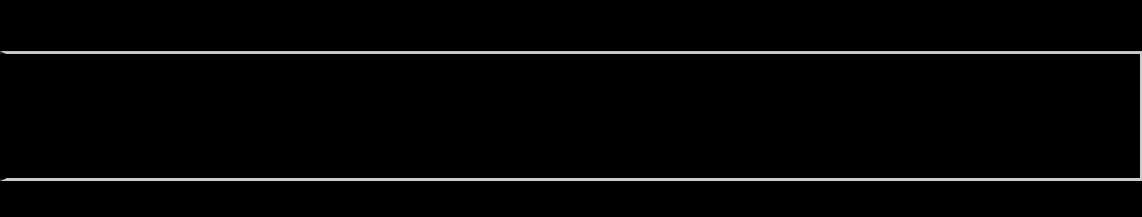
\includegraphics[width=0.9\textwidth]{informe_scratch_sinergia_p27_1142x217_5fe82248.png}
\caption{Pruebas del evaluador (material original Sinergia)}
\label{fig:tec-g-sin-tests}
\end{figure}
\begin{figure}[H]
\centering

\includegraphics[width=0.9\textwidth]{informe_scratch_sinergia_p36_1142x1535_bf5b00b5.png}
\caption{\'Arbol del repositorio (material original Sinergia)}
\label{fig:tec-g-sin-tree}
\end{figure}
\section{Motores de conjuntos y cuantificadores}
\begin{figure}[H]
\centering
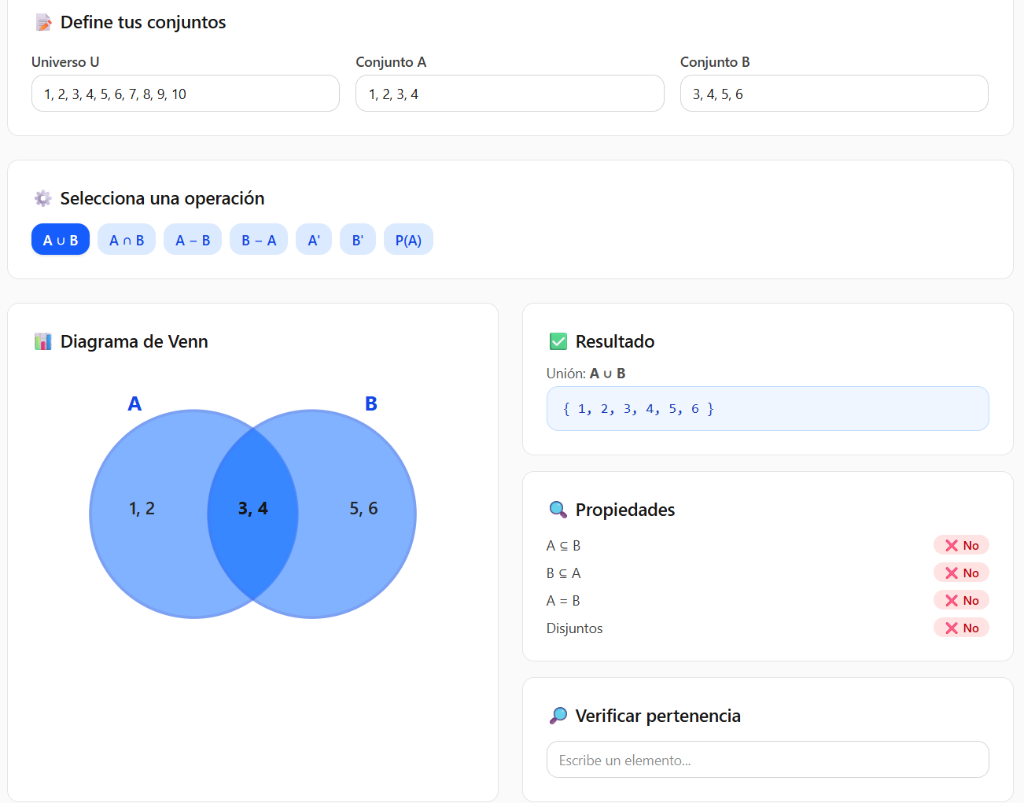
\includegraphics[width=0.85\textwidth]{informe_scratch_linus_p03_1024x803_e056eaf0.png}
\caption{Boceto inicial de conjuntos (material original Linus)}
\label{fig:tec-g-lin-wire}
\end{figure}
\begin{figure}[H]
\centering
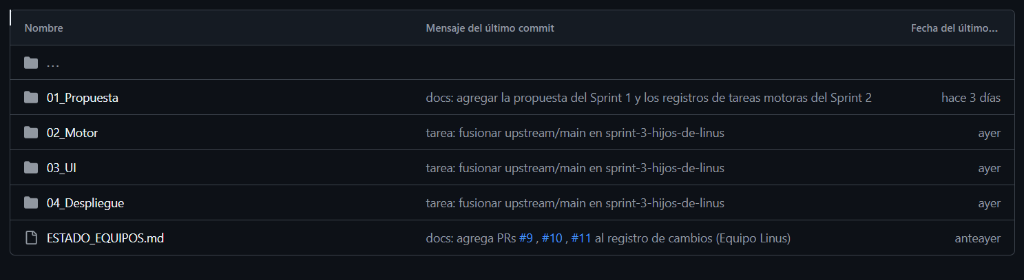
\includegraphics[width=0.9\textwidth]{informe_scratch_linus_p04_1024x280_bb5eb995.png}
\caption{Flujo Git del equipo Linus (material original)}
\label{fig:tec-g-lin-git}
\end{figure}
\begin{figure}[H]
\centering
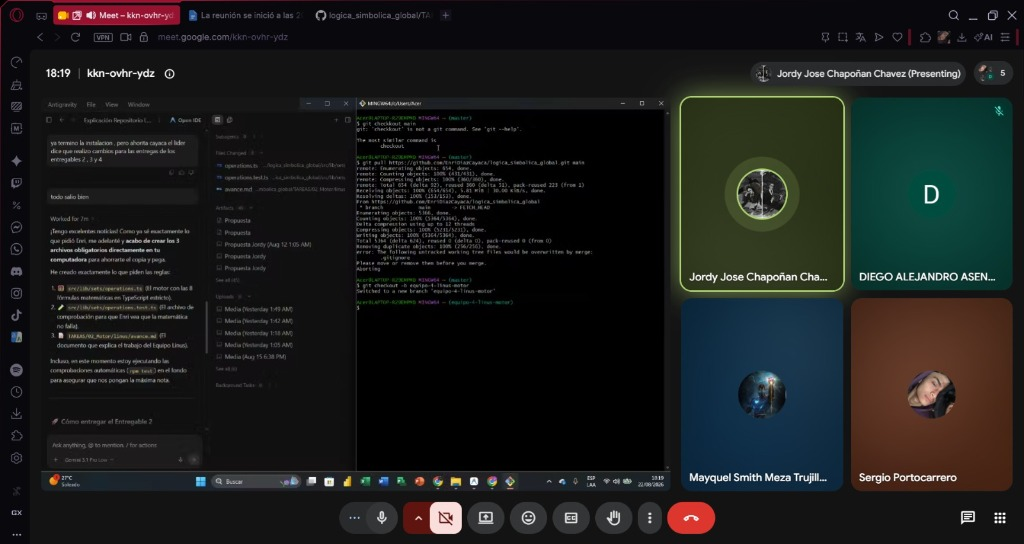
\includegraphics[width=0.9\textwidth]{informe_scratch_linus_p07_1024x544_a879fc66.jpeg}
\caption{Trabajo colaborativo Linus (material original)}
\label{fig:tec-g-lin-meet}
\end{figure}
\begin{figure}[H]
\centering
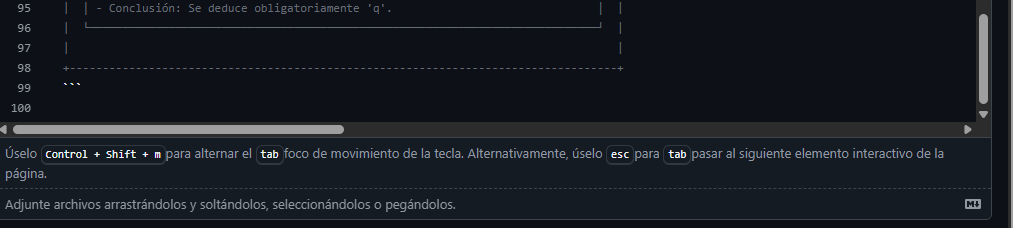
\includegraphics[width=0.9\textwidth]{informe_scratch_modusinnova_p06_1013x228_a2c880e2.png}
\caption{Boceto QuantifiWeb (material original Modus Innova)}
\label{fig:tec-g-mod-boc}
\end{figure}
\begin{figure}[H]
\centering
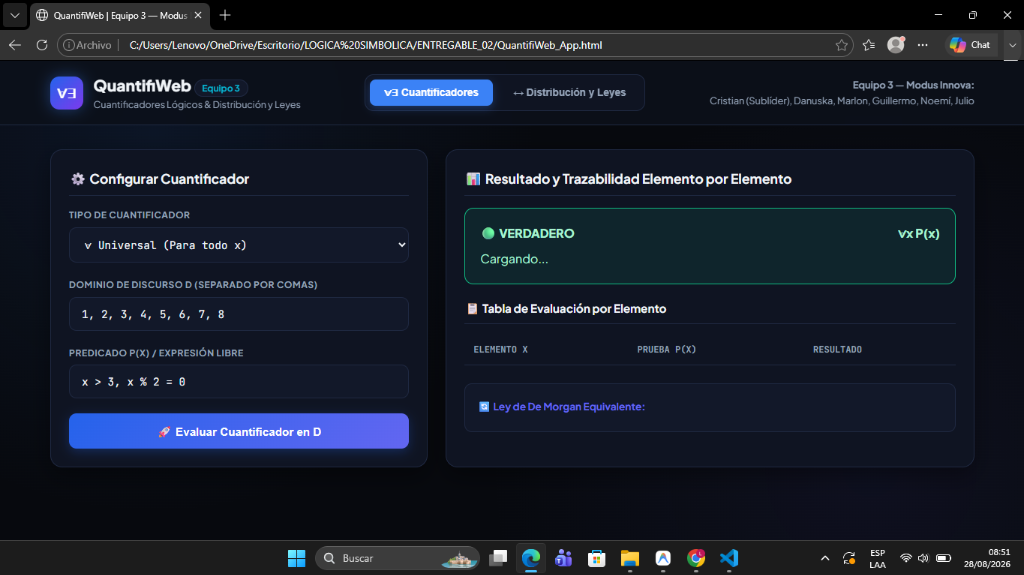
\includegraphics[width=0.9\textwidth]{informe_scratch_modusinnova_p07_1024x575_9d31f7a8.png}
\caption{Motor de cuantificadores (material original Modus Innova)}
\label{fig:tec-g-mod-mot}
\end{figure}
\begin{figure}[H]
\centering
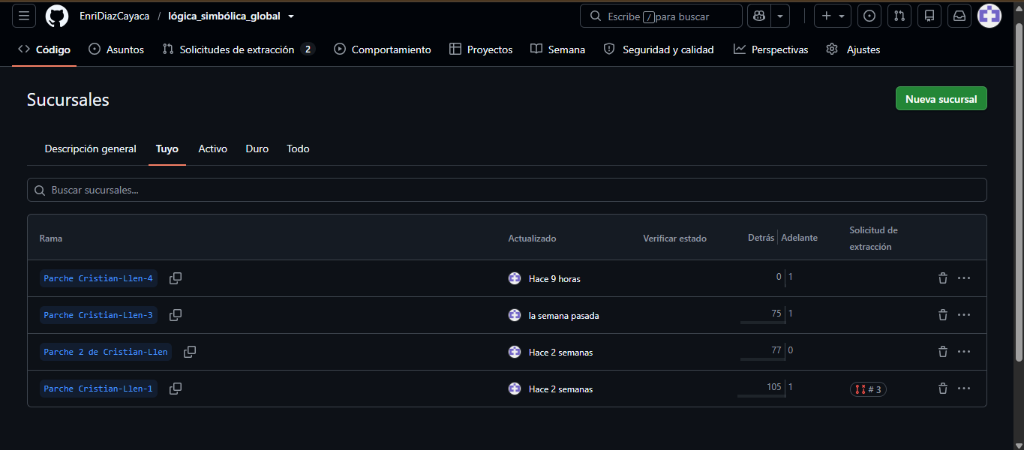
\includegraphics[width=0.9\textwidth]{informe_scratch_modusinnova_p08_1024x450_12adb3de.png}
\caption{Integraci\'on Vue (material original Modus Innova)}
\label{fig:tec-g-mod-vue}
\end{figure}
\begin{figure}[H]
\centering
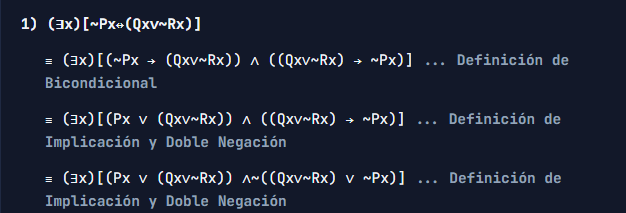
\includegraphics[width=0.9\textwidth]{informe_scratch_modusinnova_p09_626x213_e54a46e2.png}
\caption{Leyes, segunda parte (material original Modus Innova)}
\label{fig:tec-g-mod-ley2}
\end{figure}

\chapter{Validaci\'on, trazabilidad y p\'aginas}
\label{ch:val-pag}
El validador unifica m\'as de 15 notaciones hacia claves can\'onicas con prevenci\'on de inyecciones. La trazabilidad acumula pasos en orden con instant\'aneas. Las nueve vistas orquestan entradas reactivas y motores sin contener l\'ogica. El despliegue publica en Pages con vistas previas por Pull Request.
\begin{figure}[H]
\centering

\includegraphics[width=0.35\textwidth]{public_logo.jpg}
\caption{Logo institucional LogiLearn}
\label{fig:tec-logo}
\end{figure}


\chapter{Registro de decisiones de dise\~no}
\label{ch:adr-det}
En s\'intesis: Vue 3 por componentes tipados; TypeScript estricto para motores; sin almac\'en global por estado local suficiente; doble parser (caracteres frente a palabras) por dominios distintos; cotas de 12 iteraciones y 2000 elementos contra la explosi\'on; contenido externalizado para edici\'on docente sin c\'odigo.

\begin{table}[H]
\centering
\caption{Ocho decisiones con alternativa descartada}
\begin{tabular}{lll}
\toprule
Decisi\'on & Elegido & Descartado \\
\midrule
Framework & Vue 3 tipado & Alternativas sin tipado \\
Almac\'en & Estado local & Almac\'en global (innecesario) \\
Parser tablas & Por caracteres & Por palabras (ambiguo con $\land$) \\
Parser solver & Por palabras & Por caracteres (ilegible en espa\~nol) \\
Dominio & H\'ibrido + estricto & Solo libre (inseguro) \\
Reescritura & Texto plano dirigido & \'Arbol completo (costoso) \\
Iteraciones & 12 encadenadas & Ilimitadas (explosi\'on) \\
Contenido & Claves por m\'odulo & Literales en vistas \\
\bottomrule
\end{tabular}
\end{table}

\chapter{Despliegue y mantenimiento}
\label{ch:deploy-det}
\section{Procedimiento paso a paso}
\begin{enumerate}[leftmargin=*]
\item Verificar tipos y empaquetar 1860 m\'odulos con la base \texttt{/logica\_simbolica\_global/}.
\item Publicar la compilaci\'on en la rama de p\'aginas con redirecci\'on para rutas.
\item Cada Pull Request genera una vista previa temporal con URL \'unica.
\item Ante contenido antiguo, recarga forzada con Ctrl + Shift + R.
\end{enumerate}

La compilaci\'on verifica tipos y empaqueta 1860 m\'odulos. La base \texttt{/logica\_simbolica\_global/} sirve en Pages con redirecci\'on para rutas y vistas previas por Pull Request. El mantenimiento edita claves por m\'odulo con interruptor de modo literal y valida con 189 pruebas antes de publicar.

\chapter{Glosario t\'ecnico}
\label{ch:glos-tec}
\begin{description}[leftmargin=*]
\item[AST] \'Arbol de sintaxis abstracta por precedencia.
\item[Precedencia] Orden $\lnot > \land > \lor > \to > \leftrightarrow$.
\item[Forward chaining] Encadenamiento hacia adelante hasta 12 iteraciones.
\item[Contraejemplo] Asignaci\'on con premisas $V$ y conclusi\'on $F$.
\item[Testigo] Elemento que satisface un $\exists$.
\item[$D \subset \mathbb{Z}$] Dominio finito de enteros.
\item[$\Delta$] Disyunci\'on fuerte $(p \lor q) \land \lnot(p \land q)$.
\item[Modo literal] Interruptor por m\'odulo entre s\'imbolos y palabras.
\item[Trazabilidad] Pasos acumulados en orden con instant\'aneas.
\item[Potencia] $P(A)$ con $2^{n}$ subconjuntos y m\'ascara de bits.
\end{description}


\chapter{Casos de prueba nominales por archivo}
\label{ch:casos}
Cada fila reproduce el nombre declarado del caso en el repositorio. La suite total suma 189 pruebas en 17 archivos.
\begin{center}
\begin{longtable}{ll}
\caption{Casos nominales (selecci\'on de 6 por archivo)} \\
\toprule
Archivo & Caso \\
\midrule
\endfirsthead
\caption{Casos nominales (continuaci\'on)} \\
\toprule
Archivo & Caso \\
\midrule
\endhead
components/inferencias/\_\_tests\_\_/ArbolAST.test.ts & renderiza un árbol recursivo con <ul>/<li> para una implicación \\
components/inferencias/\_\_tests\_\_/ArbolAST.test.ts & respeta la precedencia de paréntesis en un único diagrama \\
components/inferencias/\_\_tests\_\_/ArbolAST.test.ts & muestra un aviso cuando la sintaxis es inválida sin romper la vista \\
components/inferencias/\_\_tests\_\_/ArbolAST.test.ts & normaliza notación matemática (P $ \to $ Q) y dibuja el árbol sin error \\
components/inferencias/\_\_tests\_\_/ArbolAST.test.ts & muestra un árbol de ejemplo cuando no hay premisas ingresadas \\
components/inferencias/\_\_tests\_\_/ArbolAST.test.ts & combina premisas y conclusión en UN solo diagrama con raíz \\
components/inferencias/\_\_tests\_\_/FormularioInferencia.test.ts & deshabilita el botón de Demostrar si las entradas están vacías \\
components/inferencias/\_\_tests\_\_/FormularioInferencia.test.ts & habilita el botón si hay premisas y conclusión \\
components/inferencias/\_\_tests\_\_/FormularioInferencia.test.ts & deshabilita el botón si isLoading es true, incluso con entradas llenas \\
components/inferencias/\_\_tests\_\_/FormularioInferencia.test.ts & emite submit normalizando símbolos a palabras clave del motor \\
components/inferencias/\_\_tests\_\_/FormularioInferencia.test.ts & inserta tokens al presionar los botones del teclado lógico con reglas de espaciado \\
components/inferencias/\_\_tests\_\_/FormularioInferencia.test.ts & borra el último carácter al pulsar el botón de borrar \\
components/inferencias/\_\_tests\_\_/IndicadorResultado.test.ts & no muestra nada si resultado es \\
components/inferencias/\_\_tests\_\_/IndicadorResultado.test.ts & renderiza caso válido demostrada \\
components/inferencias/\_\_tests\_\_/IndicadorResultado.test.ts & renderiza caso válido con método indirecto requerido \\
components/inferencias/\_\_tests\_\_/IndicadorResultado.test.ts & renderiza caso inválido refutado \\
components/inferencias/\_\_tests\_\_/IndicadorResultado.test.ts & renderiza caso error con mensaje personalizado \\
components/inferencias/\_\_tests\_\_/PanelTrazabilidad.test.ts & renderiza un mensaje si no hay pasos y no es inválido \\
components/inferencias/\_\_tests\_\_/PanelTrazabilidad.test.ts & renderiza correctamente el diagnóstico de inferencia inválida con contraejemplo \\
components/inferencias/\_\_tests\_\_/PanelTrazabilidad.test.ts & renderiza correctamente los pasos y su botón de acordeón \\
components/inferencias/\_\_tests\_\_/PanelTrazabilidad.test.ts & despliega y oculta la explicación didáctica al hacer clic en el botón \\
components/inferencias/\_\_tests\_\_/PanelTrazabilidad.test.ts & exporta el markdown académico con notación simbólica (sin palabras del motor) \\
components/inferencias/\_\_tests\_\_/PanelTrazabilidad.test.ts & exporta un documento LaTeX completo y compilable \\
components/inferencias/\_\_tests\_\_/TraductorLenguajeNatural.test.ts & detecta variables de las premisas y muestra la traducción \\
components/inferencias/\_\_tests\_\_/TraductorLenguajeNatural.test.ts & actualiza la narración cuando el usuario cambia el significado de una variable \\
lib/cuantificadores/engine.test.ts & parsea una cadena de números separados por coma \\
lib/cuantificadores/engine.test.ts & elimina espacios extra \\
lib/cuantificadores/engine.test.ts & filtra entradas vacías \\
lib/cuantificadores/engine.test.ts & parsea rango con < (excluyente) \\
lib/cuantificadores/engine.test.ts & parsea rango con <= (inclusivo) \\
lib/cuantificadores/engine.test.ts & parsea rango descendente \\
lib/integracion\_motor.test.ts & debe procesar un flujo completo: Entrada sucia -> Sanitización -> Parseo AST -> Solver -> Trazabilidad -> Transcripción \\
lib/integracion\_motor.test.ts & debe manejar entradas inválidas sin que el pipeline colapse con errores no capturados \\
lib/integracion\_motor.test.ts & debe procesar notaciones simbólicas ricas como Unicode y flechas compuestas \\
lib/sets/operations.test.ts & Unión: A $ \cup $ B combina todos los elementos sin repetir \\
lib/sets/operations.test.ts & Unión: propiedad conmutativa A $ \cup $ B = B $ \cup $ A \\
lib/sets/operations.test.ts & Intersección: A $ \cap $ B devuelve solo elementos comunes \\
lib/sets/operations.test.ts & Intersección: conjuntos disjuntos retornan vacío \\
lib/sets/operations.test.ts & Diferencia: A -- B devuelve lo que está en A pero no en B \\
lib/sets/operations.test.ts & Complemento: A\ \\
lib/solver/astVisual.test.ts & cuenta nodos y profundidad correctamente en P $ \to $ Q \\
lib/solver/astVisual.test.ts & reconoce la aridad unaria de NO \\
lib/solver/astVisual.test.ts & respeta paréntesis: NO (P $ \to $ Q) tiene a NO como raíz \\
lib/solver/astVisual.test.ts & genera estadísticas coherentes \\
lib/solver/parser.test.ts & debe tokenizar correctamente variables y operadores simples \\
lib/solver/parser.test.ts & debe aislar paréntesis sin importar los espacios \\
lib/solver/parser.test.ts & debe construir AST para expresión simple (P O Q) \\
lib/solver/parser.test.ts & debe respetar la precedencia (NO P ENTONCES Q) \\
lib/solver/parser.test.ts & debe respetar los paréntesis explícitos: NO (P ENTONCES Q) \\
lib/solver/parser.test.ts & debe lanzar error de sintaxis ante expresiones mal formadas \\
lib/solver/solver.test.ts & debe identificar variables iguales (case-insensitive) \\
lib/solver/solver.test.ts & debe rechazar variables diferentes \\
lib/solver/solver.test.ts & debe encontrar contraejemplo para la falacia de afirmación del consecuente \\
lib/solver/solver.test.ts & debe encontrar contraejemplo para la falacia del dilema inverso reportada por el usuario \\
lib/solver/solver.test.ts & debe aplicar Silogismo Disyuntivo Exclusivo (P $ \oplus $ Q y P |- $ \lnot $Q) \\
lib/solver/solver.test.ts & debe aplicar Silogismo Disyuntivo Exclusivo (P $ \oplus $ Q y $ \lnot $P |- Q) \\
lib/trazabilidad/trazabilidad.test.ts & devuelve un array vacio al inicio \\
lib/trazabilidad/trazabilidad.test.ts & registra un paso y lo retorna con datos completos \\
lib/trazabilidad/trazabilidad.test.ts & acumula multiples pasos en orden \\
lib/trazabilidad/trazabilidad.test.ts & genera estadoActual con todas las lineas disponibles \\
lib/trazabilidad/trazabilidad.test.ts & procesa un resultado valido con pasos \\
lib/trazabilidad/trazabilidad.test.ts & procesa un resultado invalido sin pasos \\
lib/truth-table/evaluator.test.ts & parsea una variable simple \\
lib/truth-table/evaluator.test.ts & parsea negación \\
lib/truth-table/evaluator.test.ts & parsea conjunción \\
lib/truth-table/evaluator.test.ts & parsea implicación con símbolo $ \to $ \\
lib/truth-table/evaluator.test.ts & parsea bicondicional con símbolo $ \leftrightarrow $ \\
lib/truth-table/evaluator.test.ts & lanza error con expresión vacía \\
lib/validator/validator.test.ts & debe rechazar cadenas vacías \\
lib/validator/validator.test.ts & debe rechazar cadenas con solo espacios, tabuladores o saltos de línea \\
lib/validator/validator.test.ts & debe normalizar espacios múltiples a un solo espacio \\
lib/validator/validator.test.ts & debe convertir variables y operadores en minúsculas a mayúsculas \\
lib/validator/validator.test.ts & CB-05: debe normalizar flechas de condicional (->, =>, $ \to $, $ \Rightarrow $, implies) \\
lib/validator/validator.test.ts & CB-06: debe normalizar bicondicionales (<->, <=>, $ \leftrightarrow $, $ \Leftrightarrow $, iff, si y solo si) \\
lib/validator/validator\_stress.test.ts & debe sanitizar y parsear expresiones con múltiples niveles de anidación de paréntesis \\
lib/validator/validator\_stress.test.ts & debe manejar expresiones con hasta 10 niveles de anidación \\
lib/validator/validator\_stress.test.ts & debe manejar cadenas con muchos operadores combinados en línea \\
lib/validator/validator\_stress.test.ts & debe admitir combinaciones mixtas de símbolos de negación (!~$ \lnot $) \\
lib/validator/validator\_stress.test.ts & debe sanitizar negaciones precediendo paréntesis: ~(p \& q) y $ \lnot $(p -> q) \\
lib/validator/validator\_stress.test.ts & debe rechazar negaciones sin operando al final de subexpresiones: (P Y NO) \\
pages/inferencias/\_\_tests\_\_/index.test.ts & realiza el flujo completo de inferencia correctamente simulando el motor \\
pages/inferencias/\_\_tests\_\_/index.test.ts & permite cambiar entre pestañas de Simbología y Lenguaje Natural \\
pages/inferencias/\_\_tests\_\_/index.test.ts & muestra el diagnóstico en el panel cuando la inferencia es inválida \\
pages/inferencias/\_\_tests\_\_/index.test.ts & muestra el mensaje de error cuando ocurre una excepción \\
test\_ejemplo.test.ts & debe ejecutar pruebas correctamente \\
\bottomrule
\end{longtable}
\end{center}

\chapter{Etapas del reescritor con ejemplo}
\label{ch:etapas}
\begin{table}[H]
\centering
\caption{Ocho etapas con transformaci\'on de ejemplo}
\begin{tabular}{ll}
\toprule
Etapa & Ejemplo \\
\midrule
Doble negaci\'on & $\lnot\lnot p \Rightarrow p$ \\
Disyunci\'on fuerte & $p \,\Delta\, q \Rightarrow (p \lor q) \land \lnot(p \land q)$ \\
Bicondicional & $p \leftrightarrow q \Rightarrow (p \to q) \land (q \to p)$ \\
Implicaci\'on & $p \to q \Rightarrow \lnot p \lor q$ \\
De Morgan & $\lnot(p \land q) \Rightarrow \lnot p \lor \lnot q$ \\
Distribuci\'on & $p \land (q \lor r) \Rightarrow (p \land q) \lor (p \land r)$ \\
Cuantificador vac\'io & $\forall x\,P \Rightarrow P$ si $x$ no ocurre \\
Simplificaci\'on repetida & aplica la misma regla hasta fijar \\
\bottomrule
\end{tabular}
\end{table}


\chapter{Demostraciones formales por tabla}
\label{ch:demos}
\section{Conectivos primitivos}
\begin{table}[H]
\centering
\caption{Tablas de los cinco conectivos}
\begin{tabular}{cc|c|c|c|c}
\toprule
$p$ & $q$ & $\lnot p$ & $p \land q$ & $p \lor q$ & $p \to q$ \\
\midrule
$V$ & $V$ & $F$ & $V$ & $V$ & $V$ \\
$V$ & $F$ & $F$ & $F$ & $V$ & $F$ \\
$F$ & $V$ & $V$ & $F$ & $V$ & $V$ \\
$F$ & $F$ & $V$ & $F$ & $F$ & $V$ \\
\bottomrule
\end{tabular}
\end{table}
El bicondicional $p \leftrightarrow q$ es $V$ cuando ambos coinciden. La precedencia $\lnot > \land > \lor > \to > \leftrightarrow$ elimina par\'entesis redundantes.
\section{De Morgan proposicional y cuantificacional}
$\lnot(p \land q)$ coincide con $\lnot p \lor \lnot q$ en las 4 filas; al negar, $\land$ se convierte en $\lor$. La versi\'on cuantificacional $\lnot(\forall x\,P(x)) \equiv \exists x\,\lnot P(x)$ se verifica por testigo y contraejemplo sobre $D$ finito.
\section{Leyes de conjuntos por extensi\'on}
$(A \cup B)^{c} = A^{c} \cap B^{c}$ se verifica elemento por elemento: $x$ est\'a a la izquierda si y solo si no est\'a ni en $A$ ni en $B$. La potencia cumple $|P(A)| = 2^{|A|}$ por inducci\'on sobre la m\'ascara binaria.

\chapter{Retrospectiva por equipo}
\label{ch:retro}
Sinergia consolid\'o el parser con 15 notaciones y la clasificaci\'on ternaria. Hijos de Linus uni\'o deducci\'on formal con evaluaci\'on exhaustiva y diagn\'ostico de siete falacias. Modus Innova restringi\'o el dominio a $D \subset \mathbb{Z}$ con cota de 2000 y reescritura dirigida. Linus separ\'o el motor puro de la vista reactiva con Venn exacto por recorte. Las cuatro bit\'acoras del anexo evidencian el avance semanal.


\chapter{Sistema de contenido por m\'odulo}
\label{ch:content-det}
\begin{table}[H]
\centering
\caption{Claves de contenido por m\'odulo}
\begin{tabular}{ll}
\toprule
M\'odulo & Claves principales \\
\midrule
Tablas & \texttt{tablas.header, .input, .info, .tablaTitulo, .explicacion} \\
Cuantificadores & \texttt{cuantificadores.header, .dominio, .predicado, .resultado} \\
Inferencias & \texttt{inferencias.titulo, .pestanas, .trazabilidad, .historial} \\
Conjuntos & \texttt{conjuntos.header, .operaciones, .diagrama, .resultado} \\
Aprender & \texttt{aprender.conectores, .etiquetasGrupo, .pasos} \\
Leyes & \texttt{leyes[12], leyesPage} \\
Global & \texttt{global.marca, .nav, .footer} \\
\bottomrule
\end{tabular}
\end{table}
Cada m\'odulo tiene su interruptor de modo literal que elige s\'imbolos ($\forall$, $\to$, $\land$) o palabras (para todo, entonces, y) sin tocar c\'odigo.

\chapter{Categor\'ias del validador en resumen}
\label{ch:val-res}
Vac\'io y blancos, espaciado, may\'usculas, flechas, bicondicionales, conjunci\'on y disyunci\'on en notaciones ASCII, negaciones, par\'entesis pegados, desbalanceados y vac\'ios, caracteres prohibidos y emojis, inyecciones HTML, sub\'indices, operadores consecutivos y negaciones anidadas: 21 categor\'ias con comportamiento esperado de sanitizar o lanzar error con mensaje.


\chapter{Gu\'ia de lectura y trabajo futuro}
\label{ch:guia-futuro}
\section{C\'omo leer este informe}
Los Cap\'itulos~\ref{ch:marco} a~\ref{ch:arq} fijan teor\'ia y arquitectura; los Cap\'itulos~5 a~8 desarrollan cada motor con esquemas y figuras; los Cap\'itulos~9 a~11 integran, prueban y despliegan; el anexo transcribe las bit\'acoras. Cada figura cita su material original.
\section{Trabajo futuro}
Exportaci\'on de tablas a CSV e imagen; modo cuestionario con tablas incompletas; verificador de equivalencias entre dos f\'ormulas; formas normales conjuntiva y disyuntiva autom\'aticas; calificaci\'on por docente; l\'ogica de primer orden completa con m\'ultiples variables; y tutor adaptativo sobre el almac\'en de progreso.


\chapter{Indice de correspondencia de figuras}
\label{ch:fig-index}
Cada figura cita su material original sin recompresi\'on. La tabla resume la correspondencia.
\begin{center}
\small
\begin{longtable}{ll}
\caption{Figuras y fuentes} \\
\toprule
Etiqueta & Pie \\
\midrule
\endfirsthead
\caption{Figuras y fuentes (continuaci\'on)} \\
\toprule
Etiqueta & Pie \\
\midrule
\endhead
fig:gantt & Cronograma del equipo Sinergia (material original) \\
tab:capas & Arquitectura en tres capas \\
fig:estructura & Estructura de archivos del proyecto (material original Sinergia) \\
fig:tec-gramatica & Gram\'atica del motor proposicional (material original Sinergia) \\
fig:tec-token & Tokenizador y normalizaci\'on (material original Sinergia) \\
fig:tec-parser & Parser descendente recursivo (material original Sinergia) \\
fig:tec-filas & Generaci\'on de filas por bits (material original Sinergia) \\
fig:tec-ast & Boceto del \'arbol sint\'actico (archivo original Hijos de Linus) \\
fig:tec-dominio & Validaci\'on del dominio entero (material original Modus Innova) \\
fig:tec-delta & Regla de disyunci\'on fuerte (material original Modus Innova) \\
fig:tec-venn & Diagrama de Venn interactivo (material original Linus) \\
fig:tec-diario1 & Propuestas Fernando y Mike (Linus, archivos originales) \\
fig:tec-diario2 & Parser del equipo Sinergia, detalle (material original) \\
fig:tec-diario3 & Propuestas Nio y Sergio (Linus, archivos originales) \\
fig:tec-diario4 & Entorno de pr\'actica del equipo Hijos de Linus (archivo original) \\
fig:tec-leyes-demo & Demostraci\'on paso a paso del motor de leyes (Modus Innova, material  \\
fig:tec-computed & Propiedades computadas de la vista (material original Sinergia) \\
fig:tec-estado & Estado reactivo de la vista de tablas (material original Sinergia) \\
fig:tec-cron & Cronograma de sprints (material original Sinergia) \\
fig:tec-linus-boc & Bocetos del equipo Linus (archivos originales) \\
fig:tec-hijos-ui & Interfaz del equipo Hijos de Linus (archivo original) \\
fig:tec-g-sin-port & Portada del informe original Sinergia \\
fig:tec-g-sin-tipos & Tipos del evaluador (material original Sinergia) \\
fig:tec-g-sin-afd & Tokenizador aut\'omata (material original Sinergia) \\
fig:tec-g-sin-parserlong & Parser, vista larga (material original Sinergia) \\
fig:tec-g-sin-parserdet & Parser recursivo en detalle (material original Sinergia) \\
fig:tec-g-sin-eval2 & Evaluaci\'on sem\'antica, continuaci\'on (material original Sinergia) \\
fig:tec-g-sin-eval3 & Evaluaci\'on y ramas (material original Sinergia) \\
fig:tec-g-sin-wrap & Envoltura del \'arbol a Unicode (material original Sinergia) \\
fig:tec-g-sin-react & Estado reactivo de la vista (material original Sinergia) \\
fig:tec-g-sin-react2 & Estado reactivo, continuaci\'on (material original Sinergia) \\
fig:tec-g-sin-comp & Propiedades computadas (material original Sinergia) \\
fig:tec-g-sin-acc & Acceso documentado (material original Sinergia) \\
fig:tec-g-sin-tests & Pruebas del evaluador (material original Sinergia) \\
fig:tec-g-sin-tree & \'Arbol del repositorio (material original Sinergia) \\
fig:tec-g-lin-wire & Boceto inicial de conjuntos (material original Linus) \\
fig:tec-g-lin-git & Flujo Git del equipo Linus (material original) \\
fig:tec-g-lin-meet & Trabajo colaborativo Linus (material original) \\
fig:tec-g-mod-boc & Boceto QuantifiWeb (material original Modus Innova) \\
fig:tec-g-mod-mot & Motor de cuantificadores (material original Modus Innova) \\
fig:tec-g-mod-vue & Integraci\'on Vue (material original Modus Innova) \\
fig:tec-g-mod-ley2 & Leyes, segunda parte (material original Modus Innova) \\
fig:tec-logo & Logo institucional LogiLearn \\
\bottomrule
\end{longtable}
\normalsize
\end{center}


\chapter{Matriz de trazabilidad requisito-evidencia}
\label{ch:traz-req}
Cada requisito acordado para esta entrega se rastrea a su secci\'on de evidencia.
\begin{table}[H]
\centering
\caption{Requisito y evidencia}
\begin{tabular}{ll}
\toprule
Requisito & Evidencia \\
\midrule
Voz \'unica & Redacci\'on unificada en todos los cap\'itulos \\
Manual solo uso & Cap\'itulos de uso sin c\'odigo interno ni Excel \\
T\'ecnico sin manual & Arquitectura, motores, sprints y anexos \\
Todas las im\'agenes originales & Galer\'ia y figuras con material sin recompresi\'on \\
Plantilla reelegida e \'indice & Portada, TOC, figuras, tablas y bibliograf\'ia global \\
Ortograf\'ia y terminolog\'ia & $D \subset \mathbb{Z}$ y conectivos unificados \\
C\'odigo necesario con diagramas & Esquemas curados y tablas de complejidad \\
Scratch fuera del repo & Solo transcripci\'on del anexo, PDFs fuera \\
TAREAS como evidencia & Anexo de bit\'acoras fieles formateadas \\
\bottomrule
\end{tabular}
\end{table}

\begin{thebibliography}{9}
\bibitem{copi2017} Copi, I. M., Cohen, C. y McMahon, K. (2017). \textit{Introducci\'on a la l\'ogica} (14.\textsuperscript{a} ed.). Pearson.
\bibitem{hurley2015} Hurley, P. J. (2015). \textit{A Concise Introduction to Logic} (12.\textsuperscript{a} ed.). Cengage.
\bibitem{suppes1971} Suppes, P. (1971). \textit{Introducci\'on a la l\'ogica simb\'olica}. Continental.
\bibitem{mendelson2015} Mendelson, E. (2015). \textit{Introduction to Mathematical Logic} (6.\textsuperscript{a} ed.). Chapman \& Hall.
\bibitem{halmos1960} Halmos, P. R. (1960). \textit{Naive Set Theory}. Springer.
\bibitem{vue2024} Vue.js Team. (2024). \textit{Vue 3 Documentation}. \url{https://vuejs.org}
\bibitem{vite2024} Vite Team. (2024). \textit{Vite Documentation}. \url{https://vitejs.dev}
\end{thebibliography}
\backmatter
\end{document}
